%\documentclass{cslthse-msc} %% Lund
\documentclass[pregrado]{tesis-usb} %% USB
\usepackage[utf8]{inputenc}
\usepackage{amsmath}
\usepackage{amsfonts}
\usepackage{amssymb}
\usepackage{amsthm}
\usepackage{amsmath}
\usepackage{mathtools}
%%\usepackage{makeidx}
\usepackage{graphicx}

\usepackage{acronym}
\usepackage{amsmath}
\usepackage{amsfonts}
\usepackage{amssymb}



%\usepackage{hyperref}
\usepackage[hyphens]{url}

\usepackage{diagbox}
\usepackage{float}
\usepackage{booktabs}
\usepackage{makecell}
\usepackage{placeins}


\DeclarePairedDelimiter\abs{\lvert}{\rvert}%
\DeclarePairedDelimiter\norm{\lVert}{\rVert}%

%\geometry{showframe}

% Spanish Changes
%\addto\captionsspanish{% Replace "english" with the language you use
%	\renewcommand{\contentsname}%
%	{Tabla de Contenidos}%
%}

%\author{
%	Christian Alexander Oliveros Labrador \\
%	{\normalsize \href{mailto:christianol_01@hotmail.com}{\texttt{christianol\_01@hotmail.com}}}
%	%\and
%	%Camilla Lekebjer \\
%	%{\normalsize \href{mailto:Camilla.Lekebjer@cs.lth.se}{\texttt{Camilla.Lekebjer@cs.lth.se}}}
%}

%\title{Muestreo Mejorado\\para \\Temporal Anti-Aliasing}
%\subtitle{Un Temporal Anti-Aliasing Mejorado con Sobel}
%%\company{The Corporation AB LTD Inc}
%\supervisors{Ángela Di Serio, \href{mailto:adiserio@ldc.usb.ve }{\texttt{adiserio@ldc.usb.ve}}}{Michael Doggett, \href{mailto:michael.doggett@cs.lth.se}{\texttt{michael.doggett@cs.lth.se}}}
%%\supervisor{John Deer, \href{mailto:jdeer@company.com}{\texttt{jdeer@company.com}}}
%\examiner{Flavius Gruian, \href{mailto:Flavius.Gruian@cs.lth.se}{\texttt{Flavius.Gruian@cs.lth.se}}}

%\date{\today}
%%\date{January 16, 2015}

% estilo de las referencias
\bibliographystyle{plain}

\autor{Christian Alexander Oliveros Labrador}
\autori{C. A. Oliveros Labrador}
\usbid{13-11000}
\titulo{Muestreo Mejorado para Temporal Anti-Aliasing}
\fecha{Septiembre~de~2018}\usarcotutor
\agno{2018}
\fechadefensa{\today}
\tutor{Ángela Di Serio}
\usarcotutor
\cotutor{Michael Doggett \mbox{(Lund)}} 
\trabajo{Trabajo de Grado}
\coord{Ingeniería de Computación} %Coloca la coordinación
\grado{Ingeniero en Computación} %coloca el postgrado
\carrera{Carrera}
\programa{Ingeniería de Computación}
%\juradouno{Ren\'e Escalante}
%\juradodos{Johana Figueroa \mbox{(UC)}}
%\juradotres{Irene Garc\'ia}
%\juradocuatro{José Luis Palacios}

\begin{document}
\selectlanguage{spanish}
\frontmatter
\maketitle
\chapter*{Dedicatoria}

Dedicado a mi papá, mi mamá, mi hermano, toda mi familia, mis amigos de Venezuela, mis amigos de todo el mundo y a todos los profesores que me han estado para mí durante el camino. 

\par Dedicado a la Universidad Sim\'on Bol\'ivar, la Universidad de Lund y a ambas comunidades universitarias.

\chapter*{Agradecimientos}

\emph{“El día que dejemos de explorar será el día en que nos comprometemos a vivir en un mundo estancado, desprovisto de curiosidad, vacío de sueños”.}
– Neil deGrasse Tyson

Tengo muchas personas para agradecer por esta increíble aventura. Viniendo de Venezuela, a más de 8000 km de distancia de Suecia, siendo la primera vez que estoy fuera de casa por tanto tiempo, la primera vez que tomo clases sólo en inglés y ser el primer estudiante de intercambio en realizar una Tesis de Maestría en el Departamento de Ciencias de la Computación de la Universidad de Lund, ha sido una experiencia que me cambió la vida.

Me gustaría agradecer a toda mi familia, especialmente a mi papá, Wilmer Oliveros; mi mamá, Raixa Labrador; y mi hermano, Jean Pierre Oliveros, por toda su ayuda y apoyo durante este viaje. Además, me gustaría agradecer a mis amigos de todo el mundo. Gracias por ayudarme a ser lo que soy en este momento y por estar conmigo todo este tiempo.

Me gustaría agradecer a mi supervisor de la Universidad de Lund, el profesor Michael Doggett, por darme esta increíble oportunidad y por ayudarme durante su transcurso. Además, me gustaría agradecer a Pierre Moreau por ayudarme en las veces que estuve estancado.
Además, me gustaría agradecer a mi supervisora de la Universidad Simón Bolívar, la profesora Angela Di Serio; y mi Coordinadora de Ingeniería de la Computación, la profesora Marlene Goncalves, por ayudarme y apoyarme en este increíble viaje.

Finalmente, me gustaría agradecer a la Universidad Lund y la Universidad Simón Bolívar, con un agradecimiento especial a la Oficina Internacional LTH; el Departamento de Ciencias de la Computación de la Universidad de Lund, la Coordinación de Ingeniería de la Computación de la Universidad Simón Bolívar; y la Dirección de Relaciones Internacionales y Cooperación de la Universidad Simón Bolívar, por permitir que los estudiantes aprovechemos estas oportunidades de desarrollo académico y de auto crecimiento.

\begin{figure}[!hbt]
	\centering
	
\includegraphics[scale=0.3]{images/univ_logotypes.png}
\end{figure}

\begin{resumen}
	\textit{Anti-aliasing} es un componente clave de los sistemas modernos de computación gráfica 3D. Para la generación de imágenes en tiempo real en aplicaciones como juegos, es importante aumentar la tasa de muestreo por píxel para mejorar la calidad general de la imagen. Pero aumentar el muestreo puede ser costoso, especialmente para las arquitecturas actuales de \textit{Shading} Diferido. Una solución innovadora a este problema es la técnica de \textit{Temporal Anti-Aliasing} (TAA), que combina muestras de cuadros previos con las muestras del cuadro actual para aumentar efectivamente la tasa de muestreo. En este proyecto de grado, exploraremos métodos para mejorar la calidad del TAA mediante el uso de detección de bordes, tanto de color como de profundidad, y la indexación de triángulos para asegurar que sólo las muestras pertenecientes a los píxeles del cuadro actual se combinen. Nuestro objetivo es reducir el efecto de \textit{ghosting} y otros artefactos creados con las implementaciones actuales de TAA. La mejora de la calidad se evaluará comparando las imágenes generadas por TAA con las imágenes base (\textit{ground truth}) generadas mediante el uso de tasas de muestreo mucho más altas, que no serían prácticas en tiempo real. El TAA mejorado se probó utilizando métricas de imágenes, en particular, MSE, PSNR y SSIM, para comparar con la implementación de TAA original y otras técnicas actuales de Anti-Aliasing. Los resultados obtenidos mostraron que las mejoras aplicadas a TAA enriquecieron la calidad de la imagen por encima de las técnicas existentes, con valores de PSNR en torno a 39 y valores de SSIM por encima de 0,99. \\
	\vspace{2cm}\par\noindent {\small{\bf Palabras Clave\/}: TAA, Sobel, Anti-Aliasing, Triangle Indexing, TRAA.}
\end{resumen}

\tableofcontents
\listoffigures
\listoftables

\chapter*{Lista de Acrónimos}
\begin{acronym}
	\acro{USB}[USB]{Universidad Sim\'on Bol\'ivar}
	\acro{ms}[ms]{Milisegundo}
	\acro{DEP}[DEP]{Decanato de Estudios Profesionales}
	\acro{PDF}[PDF]{\textit{Portable Document Format}, Documento en Formato Portable\copyright}
	\acro{PNG}[PNG]{\textit{Portable Network Graphics}, Gráficos de Red Portátiles}
	\acro{2D}[2D]{\textit{Two Dimensions}, Dos Dimensiones}
	\acro{3D}[3D]{\textit{Three Dimensions}, Tres Dimensiones}
	\acro{TAA}[TAA]{\textit{Temporal Anti-Aliasing}}
	\acro{TXAA}[TXAA]{\textit{Temporal X Anti-Aliasing}, donde la X representa alguna versión de TAA}
	\acro{TRAA}[TRAA]{\textit{Temporal Reprojection Anti-Aliasing}, TAA utilizando reproyección (técnica base de TAA)}
	\acro{SSAA}[SSAA]{\textit{Super Sampling Anti-Aliasing}, Anti-Aliasing con Super Muestreo}
	\acro{MSAA}[MSAA]{\textit{Multi Sample Anti-Aliasing}, Anti-Aliasing Multi Muestra}
	\acro{FXAA}[FXAA]{\textit{Fast Approximate Anti-Aliasing}, Anti-Aliasing Aproximado Rápido}
	\acro{SMAA}[SMAA]{\textit{Enhanced Subpixel Morphological Anti-Aliasing}, Anti-Aliasing de Mejora Morfológica de Subpíxeles}
	\acro{AA}[AA]{\textit{Anti-Aliasing}}
	\acro{NOAA}[NOAA]{No \textit{Anti-Aliasing}}
	\acro{API}[API]{\textit{Application Programming Interface}, Interfaz de Programación de Aplicaciones}
	\acro{OpenGL}[OpenGL]{\textit{Open Graphics Library}, Librería Abierta de Gráficos}
	\acro{GPU}[GPU]{\textit{Graphics Processing Unit}, Unidad de Procesamiento de Gráficos}
	\acro{GLSL}[GLSL]{\textit{OpenGL Shading Language}, Lenguaje de Shading de OpenGL}
	\acro{MSE}[MSE]{\textit{Mean Square Error}, Error Cuadrado Medio}
	\acro{RMSD}[RMSD]{\textit{Root Mean Square Deviation}, Desviación de la Raíz Media Cuadrada}
	\acro{RMSE}[RMSE]{\textit{Root Mean Square Error}, Raíz del Error Cuadrado Medio}
	\acro{PSNR}[PSNR]{\textit{Peak Signal-To-Noise Ratio}, Relación Señal a Ruido de Pico}
	\acro{SNR}[SNR]{\textit{Signal-To-Noise Ratio}, Relación Señal a Ruido}
	\acro{SSIM}[SSIM]{\textit{Structural Similarity Index}, Relación Señal a Ruido}

\end{acronym}
\clearpage

\chapter*{Notación Matemática}
\begin{tabular}{ll}
	$\ll$ & Mucho menos que\\
	$\sum\limits_{i=a}^{b}$ & Sumatoria desde $a$ hasta $b$ indexada por $i$ 
\end{tabular}

\mainmatter

\chapter[Introducción]{Introducción}
La Computación Gráfica moderna se basa en la presentación de escenas hechas de objetos representados como modelos compuestos de polígonos primitivos, siendo el triángulo el más utilizado. Esto para aprovechar su simplicidad y propiedades geométricas para crear algoritmos óptimos que manejen su renderizado (\textit{rendering}). Los triángulos están compuestos por tres vértices, cada uno de los cuales consiste en una posición y otros parámetros asociados, por ejemplo, el color o las normales del triángulo, para la interpolación.

Cuando queremos renderizar los objetos en una escena, tomamos los vértices y los enviamos por el Canal de Renderizado (\textit{Rendering Pipeline}). Allí, son procesados y mapeados a los píxeles de la pantalla con su color respectivo.

Este proceso tiene dos usos principales: Aplicaciones fuera de línea (\textit{offline}), como películas; y aplicaciones en tiempo real (\textit{online}), como los videojuegos. Cada uno de estos usos tiene sus requisitos y limitaciones, pero, para este proyecto, sólo prestaremos atención a las aplicaciones en tiempo real.

El objetivo de este proyecto es mejorar el algoritmo de \textit{Temporal Anti-Aliasing}, técnica que aumenta la calidad de las imágenes, después del proceso de mapeo de triángulos a píxeles, al mezclar cuadros previamente renderizados con los actuales.

El principal requerimiento será lograr la representación de la escena con la mayor calidad posible, con dos restricciones principales: renderizar al menos treinta cuadros por segundo, sin causar una alta pérdida de cuadros por segundo; y trabajar con una cantidad limitada de memoria y ancho de banda, porque necesitamos poder ejecutarlo en una computadora promedio o un dispositivo móvil. \cite{Doggett2017EDAN35, Shreiner2011}


\section{Definición del Problema}
\textit{Temporal Anti-Aliasing} (TAA) es una técnica en tiempo real, relativamente nueva, que proporciona buenos resultados sin incurrir en gran consumo de memoria o costos de procesamiento de otras técnicas. Las técnicas de detección de bordes y de indexación de triángulos parecen ser buenas candidatas para mejorar la calidad de TAA, al ayudar a reducir los efectos no deseados de \textit{ghosting} y desenfoque  (\textit{blurring}) creados por las implementaciones actuales de TAA.

El objetivo de este proyecto de grado es mejorar la técnica de \textit{Temporal Anti-Aliasing} mediante el uso de detección de bordes, de color y profundidad, y técnicas de indexación de triángulos para reducir el efecto de desenfoque y \textit{ghosting}, sin disminuir la calidad de la imagen renderizada o incurrir en un gran consumo de memoria o alto costo de procesamiento.


\section{Trabajos Relacionados}
La técnica más simple de \textit{Anti-Aliasing} es \textit{Super Sampling Anti-Aliasing} (SSAA, \textit{Anti-Aliasing} con Super Muestreo), que consiste en renderizar a una resolución más alta y luego reducir la imagen a la resolución requerida. Otra técnica es \textit{Multi Sample Anti-Aliasing} (MSAA, \textit{Anti-Aliasing} Multi Muestra), que calcula el color para el píxel final solo una vez \cite{Doggett2017EDAN35}. Podemos conocer ver base de lo que se conoce en la actualidad como \textit{Temporal Reprojection Anti-Aliasing} (TAA o TRAA, \textit{Anti-Aliasing} de Reproyección Temporal) en los artículos Aceleración del \textit{Shading} en Tiempo Real con Caching de Reproducción Inversa por Nehab D. et al.  \cite{Nehab2007}, en el que describen cómo se pueden usar los \textit{pixel shaders} para guardar información de los píxeles del cuadro anterior y reproyectarla en el siguiente cuadro; y Supermuestreo Amortizado por Yang L. et al.  \cite{Yang2009} en el que describen cómo utilizar la reproyección de cuadros previos  en el actual, como método de \textit{Anti-Aliasing} en tiempo real.

A continuación, encontramos técnicas de Post-Procesamiento como \textit{Fast Approximate Anti-Aliasing} (FXAA, \textit{Anti-Aliasing} Aproximado Rápido) por Timothy Lottes \cite{Lottes2009} que usa una forma de detección de bordes para corregir el \textit{aliasing} mientras es compatible con la Arquitectura de \textit{Shading} Diferido (\textit{Deferred Shading Architecture}). También tenemos la implementación de Crytek del \textit{Temporal Anti-Aliasing} (TAA o TXAA) explicada por Tiago Sousa en su presentación Métodos de \textit{Anti-Aliasing} en CryENGINE 3 \cite{JIMENEZ2011_SIGGRAPH11}.

También disponemos de la técnica \textit{Enhanced Subpixel Morphological Anti-Aliasing} (SMAA, \textit{Anti-Aliasing} de Mejora Morfológica de Subpíxeles) de Jorge Jiménez et al. \cite{Jimenez2012} que utiliza una técnica de reconstrucción de bordes más compleja, al mismo tiempo que puede trabajar con SSAA, MSAA y una forma básica de TAA.

Finalmente, tenemos las implementaciones TRAA de Ke Xu para Uncharted 4 y Lasse Fuglsang para Inside, que implementan nuevos avances como el \textit{Color Clipping Box} (Caja de Recorte de Colores) y el Filtro de Nitidez (\textit{Sharpen Filter}). Estas dos últimas implementaciones se utilizan como base de este proyecto de grado. \cite{Fuglsand2016, XU2016}


\section{Contribución}
este proyecto de grado mejora los últimos avances de Ke Xu y Lasse Fuglsang \cite{Fuglsand2016, XU2016}. Proponemos el uso del Operador de Sobel para realizar detecciones de bordes y técnicas de indexación de triángulos para detectar píxeles que se consideran con aliasing. Una vez tenemos estos píxeles detectados, usamos su información para cambiar la forma en la que se rechazan los colores de los cuadros anteriores, a fin de reducir los artefactos de \textit{ghosting} (\textit{ghosting artifacts})  y desenfoque que tiene \textit{Temporal Anti-Aliasing}.

\chapter{Marco Tecnológico}
En este capítulo, explicaremos qué herramientas se utilizaron en este proyecto de grado y las razones de su uso.

\section{C++ y el Bonobo Framework}
Utilizamos C ++ y el \textit{Bonobo Framework} para implementar todas las mejoras realizadas en este proyecto de grado. C ++ es un lenguaje de programación de propósito general, compilado, con funciones imperativas, programación orientada a objetos y administración de memoria de bajo nivel. Lo usamos por su rendimiento, especialmente para aplicaciones de computación gráfica en tiempo real, y por su amplia base de conocimiento.

El \textit{Bonobo Framework} es la base de los cursos de laboratorio de Computación Gráfica (EDAF80) y Computación Gráfica de Alto Rendimiento (EDAN35) de la Universidad de Lund. Fue desarrollado en C ++ y proporciona un motor de renderizado que encontramos fácil de modificar y usar, especialmente, como la base en la que desarrollamos nuestras mejoras.


\section{OpenGL y GLSL}
Usamos esta Interfaz de Programación de Aplicaciones (API, \textit{Application Programming Interface}) porque es la base del sistema de renderización del \textit{Bonobo Framework}, el cual modificamos para desarrollar nuestras mejoras, y por su compatibilidad multiplataforma. La Librería Abierta de Gráficos (OpenGL, \textit{Open Graphics Library}) es una API de computación gráfica de código abierto, multiplataforma, que maneja 2D y 3D, y permite abstraer al programador de interactuar directamente con la Unidad de Procesamiento de Gráficos (GPU) para lograr una renderización acelerada por hardware. Además, proporciona al programador un Canal de Renderizado de Gráficos (\textit{Rendering Pipeline}), que normalmente se implementa directamente en hardware.

Usamos el \textit{OpenGL Shading Language} (GLSL, Lenguaje de \textit{Shading} de OpenGL) para implementar TAA y nuestras mejoras, como es parte del estándar de OpenGL. GLSL es un lenguaje para \textit{shading} de alto nivel, que permite a los programadores un mayor control del Canal de Renderizado de Gráficos, sin requerir el uso del lenguaje ensamblador de OpenGL o lenguajes específicos de cada hardware.

\section{MATLAB}
Elegimos MATLAB como el entorno donde desarrollamos nuestro marco de pruebas debido a la alta calidad de sus herramientas, su amplia base de conocimientos y sus capacidades de creación rápida de prototipos.

MATLAB es un entorno de cómputo numérico multi-paradigma propietario. Comúnmente utilizado para ciencia, ingeniería y economía. Es popular para aplicaciones de procesamiento de imágenes debido a su amplia biblioteca de algoritmos para este propósito, incluidas las métricas de imágenes.



\chapter{Marco Teórico}
En este capítulo, explicaremos los conceptos teóricos que constituyen la base de este trabajo de grado, desde la teoría de base de Computación Gráfica hasta las Métricas de Imágenes utilizadas.

\section{Canal de Renderizado}
El Canal de Renderizado Gráfico son las etapas que se realizan para transformar la información de lo que queremos graficar a lo que finalmente vemos en la pantalla. El Canal de Renderizado Gráfico actual se puede simplificar en tres etapas: \textit{Vertex Shader}, que procesa la geometría asociada con los vértices y los prepara para el siguiente paso; \textit{Rasterizer}, que mapea los triángulos a píxeles en la pantalla, calcula su visibilidad e interpola los parámetros de los vértices para cada píxel cubierto por el triángulo; y el \textit{Pixel Shader} (o \textit{Fragment Shader}) que toma los píxeles visibles del \textit{Rasterizer} y los colorea. La Figura \ref{fig:graphpipeline} es un ejemplo del Canal de Renderizado simplificado.

\begin{figure}[!hbt]
	\centering
	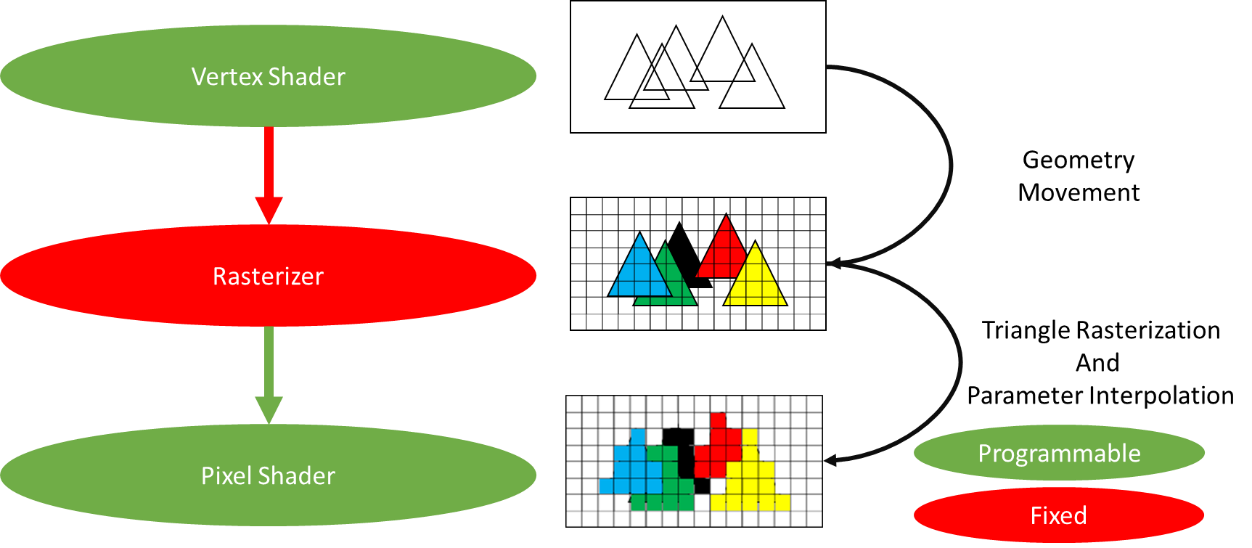
\includegraphics[scale=0.7]{images/graphics_pipeline.png} 
	\caption{Canal de Renderizado, basado en la 5ta clase de EDAF80.~\cite{Doggett2017EDAF80}}\label{fig:graphpipeline}
\end{figure}

Es importante tener en cuenta que las etapas de \textit{Vertex} y \textit{Pixel Shaders} son controlables por el programador usando programas especiales llamados \textit{Shaders}; estos proporcionan una forma para controlar el hardware de renderizado. Por el contrario, el Rasterizer no está controlado por el programador y se maneja por completo mediante una función fija de hardware. \cite{Doggett2017EDAF80}

Este proceso de rasterización es importante para este trabajo porque de allí donde provienen algunos de los errores corregidos por \textit{Temporal Anti-Aliasing}.


\section{Proceso de Rasterización}
Durante el proceso de rasterización, a cada triángulo se le realiza una prueba para establecer qué píxeles está cubriendo. Mientras se hace, cada píxel se está probando para descubrir si está cubierto por otro triángulo.

En la Figura \ref{fig:rasterizationproc} tenemos un ejemplo del Proceso de Rasterización. En la imagen de la izquierda, tenemos los triángulos como superficies continuas antes de enviarlos al \textit{Rasterizer} y, en la imagen de la derecha, tenemos triángulos mapeados a los píxeles en la pantalla después de pasar por el \textit{Rasterizer}.

\begin{figure}[!hbt]
	\centering
	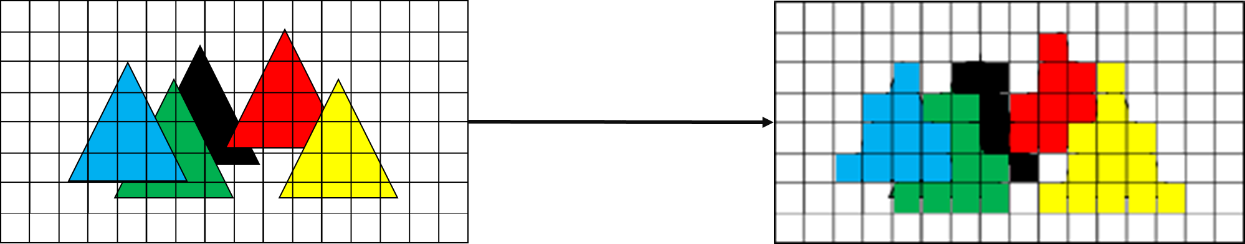
\includegraphics[scale=0.75]{images/rasterization_process.png} 
	\caption{Ejemplo de los resultados del Proceso de Rasterización.
		\emph{Nota}: se agregaron colores para diferenciar los triángulos, pero solo se agregarían en la etapa del \textit{Pixel Shader}.
	}\label{fig:rasterizationproc}
\end{figure}

Debido a que estamos mapeando un triángulo continuo a un número finito de píxeles, enfrentamos el problema de los píxeles parcialmente cubiertos y cómo determinar cuánto es suficiente para calificarlos como cubiertos, la Figura \ref{fig:partialcover} muestra ejemplos de este problema. Esto se resuelve calculando si el centro del píxel está cubierto por la geometría del triángulo. Este proceso es susceptible a errores debido a la precisión de la representación utilizada para los vértices.

\begin{figure}[!hbt]
	\centering
	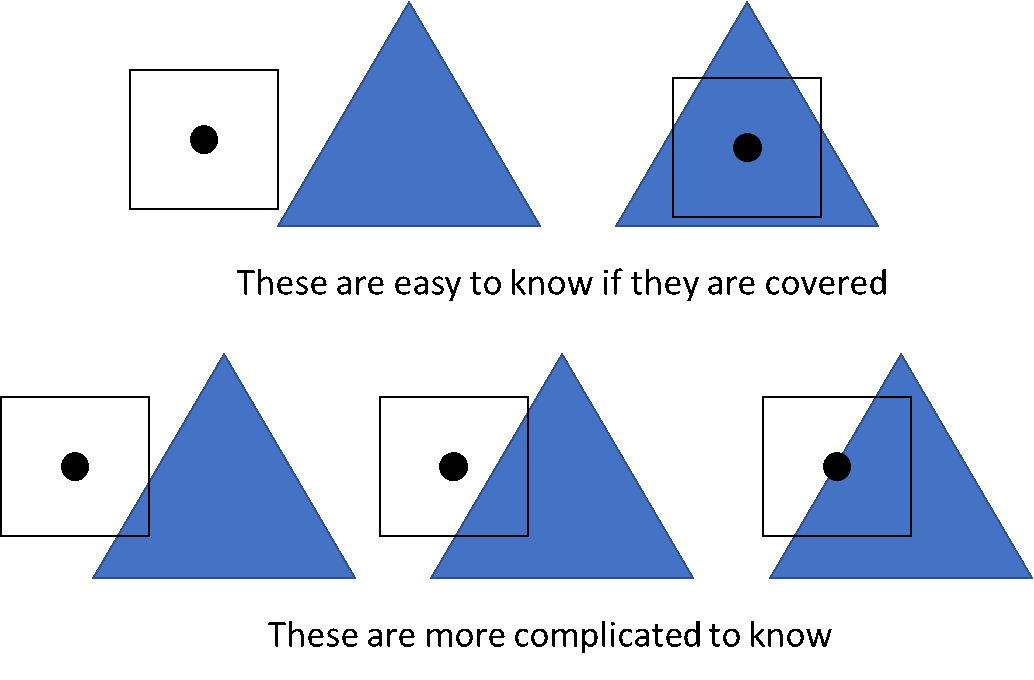
\includegraphics[scale=0.5]{images/edge_testing.png} 
	\caption{Ejemplo del problema de Cobertura Parcial, basado en la segunda clase de EDAN35. ~\cite{Doggett2017EDAN35}}\label{fig:partialcover}
\end{figure}

Este proceso nos muestra que lo que se renderiza en la pantalla, es una aproximación a lo que se representa en la escena, ya que los píxeles solo pueden ser cubiertos con un triángulo a la vez. \cite{Moller2007, Doggett2017EDAN35}


\section{El Problema del Aliasing}
Cuando mapeamos una representación continua en una finita, se generan errores. Como explican Edward Angel y Dave Shreiner en su libro (página 413) \cite{Shreiner2011}, podemos interpretar el proceso de renderización como el muestreo de una función continua $f(x, y)$, que representa el color de la escena en ese punto, a una cuadrícula de píxeles $n\times m$ en la que suponemos que el punto $f_{ij}$ es el valor de $f$ sobre un área pequeña; reconstruyendo la función $f$, para mostrar la imagen en la pantalla, usando solo lo que sabemos de las muestras finitas. La herramienta matemática utilizada para evaluar los problemas de este proceso es el Análisis de Fourier, que establece que una función se puede descomponer en un conjunto de sinusoides, posiblemente en un número infinito de frecuencias. Para el análisis de imágenes bidimensionales, podemos pensar en la función $f$ como un conjunto de sinusoides en dos frecuencias espaciales.

Para este proyecto de grado, usaremos la primera parte del Teorema de Muestreo de Nyquist, como una herramienta para ilustrar por qué aparecen problemas de aliasing y se relacionan con problemas de muestreo. \\

\emph{'' Teorema de Muestreo de Nyquist (Parte 1): Las muestras ideales de una función continua contienen toda la información de la función original si y sólo si la función continua se muestrea a una frecuencia mayor que el doble de la frecuencia más alta en la función. }

\emph{La Frecuencia de Nyquist se define como la mitad de la frecuencia de muestreo, que es la frecuencia más baja que no puede estar en los datos para evitar el \textit{aliasing} ''.
} 


Tomado de la página 415 del libro de Edward Angel y Dave Shreiner. \cite{Shreiner2011} \\

Como explican Edward Angel y Dave Shreiner, este muestreo idealizado supone que podemos tomar un número infinito de muestras por frecuencia de muestreo, que no podemos hacer en la práctica. El Problema de \textit{Aliasing} que se experimenta en la Computación Gráfica, proviene de no poder tomar muestras según lo requerido por el Teorema de Muestreo de Nyquist, creando bordes desiguales que aparecen en el proceso de rasterización (\textit{Aliasing} Espacial) y saltos entre objetos en movimiento (\textit{Aliasing} Temporal), de acuerdo con Doggett y Wronski ~\cite{Doggett2017EDAN35, Wronski2014}. La Figura \ref{fig:aliasingexample} muestra un ejemplo de Aliasing Espacial. Se han propuesto y utilizado muchas soluciones para resolver el problema de \textit{Aliasing}, como por ejemplo la familia de soluciones \textit{Super Sampling Anti-Aliasing} (SSAA), que trabaja con frecuencias más altas que las requeridas a costa de mayores requerimientos de espacio.

\begin{figure}[!hbt]
	\centering
	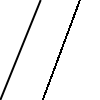
\includegraphics[scale=0.6]{images/aliasing_example.png} 
	\caption{Imagen Base de una línea frente a su Aproximación con \textit{Aliasing}.}\label{fig:aliasingexample}
\end{figure}

\section[Mapeado de Sombras y la Arquitectura de Shading Diferido]{Mapeado de Sombras y \\ la Arquitectura de Shading Diferido}

Como humanos, esperamos que los objetos reaccionen de cierta forma a las luces de una escena, tomando en cuenta la geometría de los objetos, porque las luces y sombras contribuyen con la información espacial a una imagen. En especial, las sombras nos dan una sensación de tamaño y distancia.

Según lo explicado por Doggett \cite{Doggett2017EDAN35}, bajo el Canal de Renderizado Gráfico basado en el Rasterizer , el proceso de cálculo de la sombra es difícil de realizar. El \textit{Rasterizer} no sabe si los objetos están cubiertos o no por una fuente de luz, por lo que debemos encontrar un método para calcular si un objeto está en la sombra. Este proceso se denomina Mapeado de Sombras y consiste en la representación de la escena a través de la perspectiva de cada  fuente de luz y luego realizar pruebas en la perspectiva de la cámara, para establecer si el objeto se ve afectado por la luz o si está en sombras.

Pero, como es de esperar, renderizar la escena varias veces es costoso y necesitamos una forma de reducir el costo tanto como podamos. La Arquitectura de \textit{Shading} Diferido proporciona esa solución para realizar el \textit{Shading}, utilizando una operación que podría ser costosa, a solo píxeles visibles y así evitar desperdiciar recursos realizando el \textit{Shading} a píxeles de geometrías que están cubiertas por por píxeles de otros objetos. Esta arquitectura funciona renderizando primero la escena, sin cálculos de \textit{Shading}, en un buffer llamado Buffer de Geometría (\textit{Geometry Buffer}). Allí, se guarda información sobre colores, normales, profundidades, información específica del objeto para interactuar con luces, etc. para uso futuro. 

Después de llenar el Buffer de Geometría, llevamos a cabo la técnica de Mapeado de Sombras, que aprovecha la Arquitectura de \textit{Shading} Diferido para calcular la forma en que las luces afectan sólo a los píxeles visibles; calculamos el Mapa de Sombreado de cada fuente de luz realizando cálculos de profundidad únicamente. Posteriormente, calculamos y guardamos el efecto de cada luz usando los Mapas de  Sombreado.

Al final, tomamos la información de las luces, sombras y el Buffer de Geometría para renderizar la escena con iluminación.


\section{Anti-Aliasing}
Como hemos explicado, hay dos tipos principales de \textit{Aliasing}, Espacial y Temporal. Las soluciones \textit{Anti-Aliasing} proporcionan mejoras contra los artefactos creados por cualquiera de esos tipos a costa de un mayor tiempo de renderizado. Para aplicaciones en tiempo real, este aumento del tiempo de renderización limita qué soluciones Anti-Aliasing son factibles de aplicar.

Otro factor importante para decidir qué técnica \textit{Anti-Aliasing} utilizar,  es cómo se comporta con las arquitecturas actuales. Por ejemplo, las primeras  soluciones Anti-Aliasing no funcionan con el \textit{Shading} Diferido.


\subsection{Super Sampling Anti-Aliasing (SSAA)}
Esta técnica consiste en renderizar la escena a $4$ veces el tamaño de la pantalla y luego promediar el área $4\times 4$ alrededor de cada pixel para calcular el resultado \cite{Doggett2017EDAN35}. Proporciona buenos resultados, pero requiere más tiempo de renderizado y un gran uso de memoria.

\subsection{Multi Sample Anti-Aliasing (MSAA)}
MSAA consiste en tomar varias muestras por píxel; en cada muestra, se calculan los valores de profundidad, pero solo se computa un color para el triángulo rasterizado. Esta solución proporciona buenos resultados a costa de un mayor uso de memoria para cálculos de profundidad.

El mayor problema que tiene esta técnica es que no funciona correctamente con el \textit{Shading} Diferido \cite{Doggett2017EDAN35}. Esto hace que sea complicado de utilizar con los Canales de Renderización actuales, que normalmente requieren otras correcciones para reducir los artefactos creados cuando se aplica con \textit{Shading} Diferido.


\subsection{Fast Approximate Anti-Aliasing (FXAA)}
FXAA es una técnica de \textit{Anti-Aliasing} que se utiliza durante el post-procesamiento. Esta funciona al detectar bordes en las imágenes renderizadas, para luego suavizarlos. \cite{Lottes2009}

Es relativamente barata en comparación con MSAA y proporciona resultados relativamente buenos, sus capacidades de suavizado están limitadas por la cantidad de información que la detección de bordes puede obtener en una sola pasada y proporciona resultados relativamente buenos para el \textit{Aliasing} Temporal.

\subsection{Enhanced Subpixel Morphological Antialiasing (SMAA)}
SMAA es una técnica de post-procesamiento basada en \textit{Morphological Anti-Aliasing} (Anti-Aliasing Morfológico). Funciona mediante la reconstrucción de bordes y sus alrededores para regenerar la información de subpíxel perdida por \textit{aliasing}. \cite{Jimenez2012}

\section{Temporal Anti-Aliasing}
Como explicaron Ke Xu y Lasse Fuglsang en sus respectivas presentaciones ~ \cite{XU2016, Fuglsand2016}, el principio básico del \textit{Temporal Anti-Aliasing} es mezclar el cuadro que actualmente está siendo renderizado con cuadros del pasado. Esto se hace para aumentar el número de muestras a través del tiempo en lugar de solo usar muestras del mismo cuadro.

Una de esas técnicas es \textit{Temporal Reprojection Anti-Aliasing}  (TRAA, \textit{Anti-Aliasing} de Reproyección Temporal), que funciona guardando los cuadros pasados en un Buffer de Historia para luego reproyectarlos a la escena actual y mezclarlos con el cuadro actual que se está procesando. Para lograrlo, tomamos el cuadro actual y buscamos el color que debería tener en el Buffer de Historia; este paso se llama \textit{Reprojection} (Reproyección).

Para que TRAA funcione, debemos implementar otras técnicas comunes de computación gráfica para que sirvan de base. Necesitamos de \textit{Camera Jittering} (Agitamiento de Cámara) para poder reconstruir la información de píxeles alrededor de los bordes. Un Buffer de Velocidad para determinar las posiciones de los píxeles en el último cuadro, si se movían. Un Buffer de Historia de cuadros donde recopilar los pixeles anteriores para realizar las reproyecciones en el siguiente cuadro. Un \textit{Color Clipping Box} (Caja de Recorte de Colores) para restringir el Buffer de Historia y evitar que aparezca ruido o colores incorrectos. Un Filtro de Nitidez (\textit{Sharpen Filter}) para reducir parte del desenfoque creado y \textit{Motion Blur} (Desenfoque por Movimiento) para corregir los efectos de objetos que se mueven demasiado rápido para el cuadro de recorte de colores.


\subsection{Camera Jittering}
\textit{Camera Jittering} (Agitamiento de Cámara) consiste en mover la cámara vertical y horizontalmente utilizando una traslación de subpíxeles, la Figura \ref{fig:camerajittering} es un ejemplo de la traslación horizontal. Se aplica en cada cuadro para conservar información de fragmentos de regiones locales de superficies en la escena. Si el cuadro actual se deja estático en relación con los pasados, es decir, es idéntico a los cuadros anteriores, se pierde información subpíxel alrededor de los bordes que podría usarse para refinar la imágen final.  ~\cite{Fuglsand2016, XU2016}

\begin{figure}[!hbt]
	\centering
	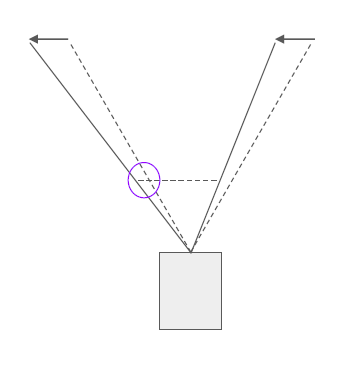
\includegraphics[scale=0.3]{images/camera_jitter.png}
	\caption{Proceso de \textit{Jittering} sobre la proyección de la cámara. Imagen tomada de la presentación de Fuglsand. \protect\cite{Fuglsand2016}}\label{fig:camerajittering}
\end{figure}

El \textit{Jittering} se aplica como una traslación a la matriz de proyección de la cámara usando la $Halton$ $Sequence$ $(2,3)$ (Secuencia de Halton 2D utilizando 3 como base) como los vectores de traslación. Esta secuencia se usa porque genera un patrón irregular para las traslaciones, que ayuda a conservar más información que un patrón regular y porque la Secuencia de Halton, proporciona un generador económico de patrones pseudoaleatorios. ~\cite{Fuglsand2016, XU2016}

\begin{figure}[!hbt]
	\centering
	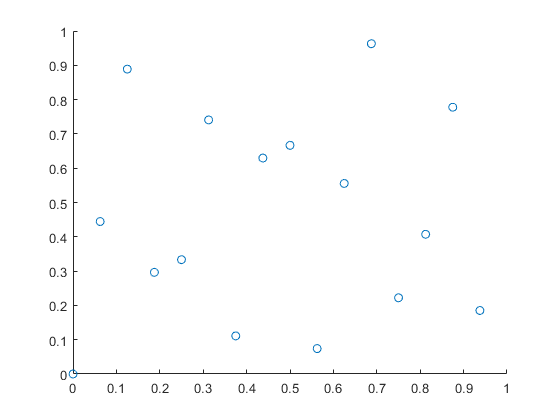
\includegraphics[scale=0.5]{images/halton_16.png}
	\caption{Valores usados de la $Halton$ $Sequence$ $(2,3)$ (Secuencia de Halton).}\label{fig:halton16}
\end{figure}

La Figura ~\ref{fig:halton16} muestra la representación de los 16 puntos utilizados para trasladar la proyección en la implementación actual del Proyecto de Grado, tal como lo propusieron Fuglsand ~\cite{Fuglsand2016}. Los puntos se generaron usando MATLAB y luego se codificaron para mejorar su aleatoriedad usando reverse-radix scrambling.

\subsection{Buffer de Velocidad}
El algoritmo de Buffer de Velocidad (Velocity Buffer) utilizado en esta implementación es el propuesto por Chapman ~\cite{Chapman2012}, el cual es calculado restando la posición actual del píxel de su posición en el cuadro pasado. Esto es posible ya que guardamos la matriz que representa cada objeto en la escena y la utilizamos en el siguiente cuadro para calcular los píxeles del Buffer de Velocidad. Además, cancelamos matemáticamente el Cámara Jittering antes de calcular las velocidades, para evitar el ruido que crea, como lo sugiere Xu. ~\cite{XU2016}


\subsection{Buffer de Historia}
Para cada fragmento en el marco actual, buscamos en la vecindad de $3\times 3$ y en la vecindad del patrón Cruz $(+)$ alrededor de cada píxel (Ver figura ~\ref{fig:samplingpattern}). Buscamos en ambos patrones para el mínimo y el máximo de colores del cuadro actual, luego los promediamos y los usamos para construir parte del Color Clipping Box restringiendo los píxeles del Buffer de Historia. ~\cite{Fuglsand2016}
\begin{figure}[!hbt]
	\centering
	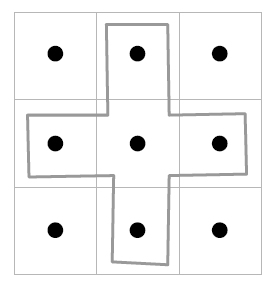
\includegraphics[scale=0.8]{images/sampling_pattern.png}
	\caption{Patrón de Muestreo utilizado. Imagen tomada de la presentación de Fuglsand. \protect\cite{Fuglsand2016}}\label{fig:samplingpattern}
\end{figure}

En la vecindad $3\times 3$ buscamos la velocidad del píxel con la profundidad más cercana a la cámara, esto es para obtener mejores bordes en movimiento para los píxeles que están ocultos detrás de otros ~\cite{Fuglsand2016}. Usamos esta velocidad para reproyectar la posición del píxel del cuadro actual en el Buffer de Historia. ~\cite{Fuglsand2016, XU2016}

Después de tener los píxeles en el Buffer de Historia, lo restringimos (explicación en la siguiente subsección) y lo interpolamos linealmente con el cuadro actual (Ver la Figura \ref{fig:samplingprocess} para obtener una representación visual del proceso completo). Interpolamos linealmente los píxeles del Buffer de Historia y el cuadro actual usando un valor de retroalimentación, que se calcula por la diferencia de luminancia entre los colores del Buffer de Historia restringido y el cuadro actual. Este valor de retroalimentación es sesgado a favor de mantener el color del Buffer de Historia del píxel sobre el color del cuadro actual, esto se hace para agregar información del cuadro actual mientras se mantiene la mayor parte de la historia del píxel. Esta interpolación lineal estabiliza la imagen, eliminando el \textit{Jittering} y suavizando los bordes ~\cite{Fuglsand2016, XU2016}. Dado que el historial de cada píxel se acumula en el Buffer de Historia, obtenemos el efecto que el historial de píxeles de los cuadros anteriores pese menos cuanto más tiempo sea mantenido el historial del píxel dentro Buffer de Historia. ~\cite{Fuglsand2016}

\begin{figure}[H]
	\centering
	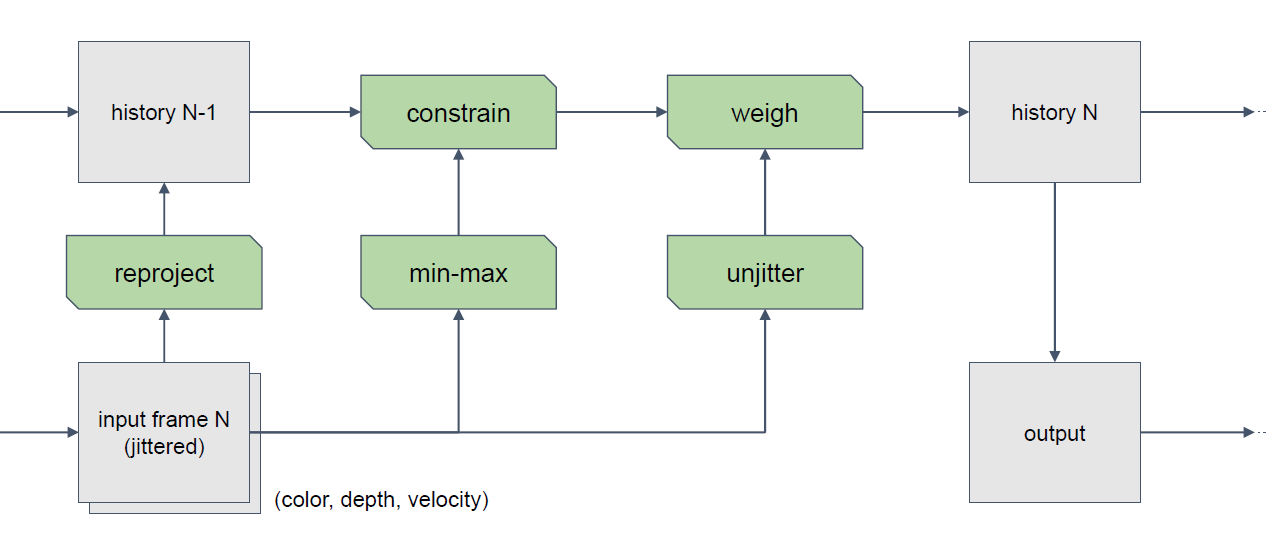
\includegraphics[scale=0.4]{images/sampling_process.png}
	\caption{Proceso de \textit{Temporal Reprojection Anti-Aliasing}. Imagen tomada de la presentación de Fuglsand \protect\cite{Fuglsand2016}}\label{fig:samplingprocess}
\end{figure}

\subsection{Clipping Color Box} 
La \textit{Clipping Color Box} (Caja de Recorte de Colores) es una caja 3D construida utilizando el color de píxel actual como el centro y el color mínimo y máximo calculado en la última subsección como los límites. Se utiliza para manejar el rechazo de la historia, cuando el color del píxel en el Buffer de Historia está muy alejado del color actual. Tomamos el color de la historia como un vector y luego lo proyectamos contra los bordes de la caja; si se encuentra fuera del borde de la caja, mantenemos la proyección; de lo contrario, el color de la historia quedará intacto. El uso del Clipping Color Box evita la agrupación de colores en las esquinas que ocurriría si se aplicara \textit{clamping} (Ver Figura ~\ref{fig:clippingbox}) ~\cite{Fuglsand2016}.

\begin{figure}[!hbt]
	\centering
	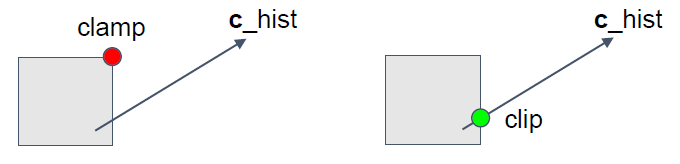
\includegraphics[scale=0.4]{images/clipping_box.png}
	\caption{\textit{Color Clamping} versus \textit{Color Clipping}. Imagen tomada del \textit{paper} de Fuglsand. \protect\cite{Fuglsand2016}}\label{fig:clippingbox}
\end{figure}


\subsection{Filtro de Nitidez} 
El Proceso de Reproyección y el \textit{Clipping} de Colores crean imágenes borrosas, por lo que se requiere un Filtro de Nitidez. Usamos el filtro propuesto por Xu. ~\cite{XU2016}

\begin{equation} \label{eq:sharpen}
\begin{bmatrix*}[r]
0 & -1 &  0 \\
-1 &  5 & -1 \\
0 & -1 &  0
\end{bmatrix*}
\end{equation}

La Ecuación \ref{eq:sharpen} representa la matriz de convolución utilizada como Filtro de Nitidez en el \textit{paper} de Xu. \protect\cite{XU2016}

\subsection{Motion Blur}
Debido a la naturaleza del Buffer de Historia, algo de \textit{ghosting} es creado por algunos fragmentos de objetos que se mueven más rápido que el tiempo que tarda el \textit{Clipping Color Box} para rechazar el color de píxeles antiguos, esto es especialmente notable bajo condiciones especiales de luz y fondo. Fuglsand y Xu ~\cite{Fuglsand2016, XU2016} propusieron usar soluciones como \textit{Motion Blur} para ocultar estos artefactos.

El \textit{Motion Blur} utilizado es el propuesto por Chapman ~\cite{Chapman2012}. Intenta comportarse como una cámara real, escalando la velocidad de cada píxel mediante la división de los cuadros actuales por segundo (FPS) a la velocidad deseada, simulando así la velocidad de obturación. Luego, mezcla los colores de los píxeles que se muestrean al seguir la dirección del vector del Buffer de Velocidad.


\subsection{Problemas}
Temporal Anti-Aliasing tiene dos inconvenientes principales, el efecto de \textit{Ghosting} de los objetos en movimiento y el Desenfoque proveniente de la forma en que funciona el \textit{Clipping Color Box}. este proyecto de grado pretende ayudar a reducir los efectos de estos dos inconvenientes utilizando nuevos enfoques. Por completitud, presentamos algunas de las soluciones actuales disponibles.

\subsubsection{Desenfoque} 
Las implementaciones actuales de TAA generan un desenfoque muy agresivo debido a la forma en que mezclan los colores del cuadro actual y el historial; el uso de áreas más grandes que el píxel aumenta los errores generados, por lo tanto, se requiere un Filtro de Nitidez. El filtro aplicado en la implementación es el utilizado por Xu ~\cite{XU2016}, que resuelve el desenfoque razonablemente bien, pero no logra eliminar algunos artefactos. 

\subsubsection{Ghosting} 
Algunos artefactos de \textit{Ghosting} se crean cuando los objetos se mueven, especialmente bajo condiciones particulares de luz y fondo, que hacen que el primer plano y el fondo se vean de manera similar. Esto se corrige parcialmente con \textit{Motion Blur}, sin embargo, parte del \textit{Ghosting} permanece cerca de objetos que se mueven lo suficientemente rápido como para crearlo, pero son lo suficientemente lentos como para evitar el \textit{Motion Blur}. Xu propone el uso de \textit{Motion Blur} y aumentar el tamaño de todo utilizando una técnica \textit{Stencil} y el etiquetado manual de objetos ~\cite{XU2016}, pero nuestro objetivo es evitar que los artistas etiqueten manualmente y prueben objetos por sus comportamientos bajo \textit{Ghosting}. La implementación de Pederson permite el \textit{Jittering} en los cálculos del Buffer de Velocidad para evitar \textit{Ghosting} en las imágenes, pero crea desenfoque no deseado. ~\cite{Fuglsand2016}. 

\section{Buffer de Acumulación}
El Buffer de Acumulación es una técnica de \textit{Anti-Aliasing} que consiste, según Paul Haeberli y Kurt Akeley \cite{Haeberli1990}, en renderizar la escena varias veces aplicando \textit{Jittering} a la cámara y luego realizar una suma ponderada a escala de las renderizaciones para generar el cuadro actual.

Este es un proceso que aumenta el muestreo por píxel y reduce los efectos de \textit{aliasing}, lo que produce una imagen de alta calidad a costa de procesar todo varias veces por cuadro.

\section{Operador de Sobel}
El Operador Sobel es un operador de gradiente isotrópico $3\times 3$ computable eficientemente, como lo explica Irwin Sobel \cite{Sobel2014}. Usamos este operador para detectar bordes en las imágenes renderizadas y marcarlos como posibles lugares con aliasing. Esto es porque los bordes son lugar común para que aparezcan los artefactos de aliasing. 

Funciona al tomar las cuatro estimaciones posibles del gradiente simple central en un vecindario de $3\times 3$ y sumarlas. La función de imagen se toma como una función de densidad / intensidad y las cuatro estimaciones posibles como vectores ortogonales que son derivadas direccionales, multiplicadas por un vector unitario que especifica la dirección de la derivada. La suma de las cuatro estimaciones posibles de gradiente simple central es equivalente a la suma vectorial de los ocho vectores derivativos direccionales.

\begin{equation}
\begin{bmatrix*}[r]\label{eq:sobel_neighborhood}
a & b & c \\
d & e & f \\
g & h & i
\end{bmatrix*}
\end{equation}

Siendo la Matriz \ref{eq:sobel_neighborhood} el Vecindario $3\times 3$ y $\abs*{G}$ la magnitud de la estimación derivada direccional del vecindario.

La dirección de $G$ estará dada por el vector unitario asociado al vecino apropiado. La suma vectorial hace que se cancelen todos los valores de $e$ (centro del Vecindario $3\times 3$) dejando la siguiente expresión \ref{eq:sobel_simplification}:
\begin{equation}\label{eq:sobel_simplification}
\begin{split}
	G & =\frac{c-g}{4}*\begin{bmatrix*}1 & 1\end{bmatrix*}+\frac{a-i}{4}*\begin{bmatrix*}-1 & 1\end{bmatrix*}+\frac{b-h}{2}*\begin{bmatrix*}0 & 1\end{bmatrix*}+\frac{f-d}{2}*\begin{bmatrix*}1 & 0\end{bmatrix*} \\ & =\begin{bmatrix*}\frac{c-g-a+i}{4}+\frac{f-d}{2} & \frac{c-g+a-i}{4}+\frac{b-h}{2}\end{bmatrix*}
\end{split}
\end{equation}

Luego multiplicamos por $4$ para aproximar el valor y asegurarnos que no perdemos precisión si lo realizamos con enteros pequeños de punto fijo. La magnitud recién calculada es dieciséis veces más grande que el gradiente promedio original.

\begin{equation}\label{eq:sobel_approximation}
\begin{split}
G' = 4 * G =\begin{bmatrix*}(c-g-a+i)+(f-d)*2 & (c-g+a-i)*4+(b-h)*2\end{bmatrix*}
\end{split}
\end{equation}

La Ecuación \ref{eq:sobel_approximation} se puede expresar en dos matrices de ponderación. Usamos la Matriz \ref{eq:sobel_x} para el componente $x$ y la Matriz \ref{eq:sobel_y} para el componente $y$.

\begin{equation}
\begin{bmatrix*}[r]\label{eq:sobel_x}
-1 &  0 & +1 \\
-2 &  0 & +2 \\
-1 &  0 & +1
\end{bmatrix*}
\end{equation}

\begin{equation}
\begin{bmatrix*}[r]\label{eq:sobel_y}
+1 & +2 & +1 \\
 0 &  0 &  0 \\
-1 & -2 & -1
\end{bmatrix*}
\end{equation}

Para la detección de bordes, lo que se hace comúnmente es comparar la magnitud de $G$ contra un umbral numérico, para marcar píxels como bordes.

\section{Métricas de Imagen}
El proceso de medir la calidad de una imagen es complicado. Como explican Al-Najjar y Soong \cite{Yusra2012}, podemos seguir dos métodos principales: subjetivos u objetivos. Los métodos subjetivos se basan en opiniones recogidas de humanos y, como cabría esperar, se consideran costosos, difíciles de implementar y llevan mucho tiempo. El segundo tipo de métodos, los objetivos, se basan en fórmulas matemáticas y algoritmos para medir la calidad de la imagen sin intervención humana. Para este proyecto de grado, usamos métodos objetivos.

Los métodos objetivos se pueden categorizar en tres grupos, como describen Al-Najjar y Soong \cite{Yusra2012}:

\begin{itemize}
	\item \textbf{Sin-Referencia:} En el cual no tenemos una imagen de referencia para comparar.
	\item \textbf{Referencia-Reducida:} Donde tenemos parte de una imagen de referencia.
	\item \textbf{Referencia-Completa:} Tenemos la imagen de referencia completa.
\end{itemize}


Para Computación Gráfica, los métodos preferidos son los de Referencia-Completa, porque las imágenes de referencia se pueden generar utilizando algoritmos de mayor calidad pero con mal rendimiento para representarlos. Las métricas más comunes utilizadas, y utilizadas en este proyecto de grado, son: Error Cuadrado Medio (MSE, \textit{Mean Square Error}); Relación Señal a Ruido de Pico (PSNR, \textit{Peak Signal-to-Noise Ratio}); y el Índice de Similitud Estructural  (SSIM, \textit{Structural Similarity Index}).

\subsection{Error Cuadrado Medio (MSE)}
Basada en el promedio del error cuadrado entre los píxeles de la imagen y la referencia. 

\begin{equation}\label{eq:mse}
	MSE=\frac{1}{N*M}\sum\limits_{i=0}^{N-1}\sum\limits_{j=0}^{M-1}(Im(i,j)-Ref(i,j))^2
\end{equation}
Donde $N, M$ son el ancho y largo de las imágenes y $Im, Ref$ son el píxel de la Imagen y la Referencia.

\subsection{Desviación de la Raíz Cuadrada Media  (RMSD)}
Es la desviación estándar de MSE (\textit{Root Mean Square Deviation}). También llamada \textit{Root Mean Square Error} (RMSE).
\begin{equation}\label{eq:rmse}
RMSE=\sqrt{MSE}
\end{equation}

\subsection{Relación Señal a Ruido de Pico (PSNR)}
Se basa en el concepto matemático de Relación de Señal a Ruido (SNR, Signal-To-Noise Ratio) que mide la señal de la imagen, que se almacena como los colores de los píxeles para nuestros propósitos, contra su error en comparación con la referencia. \cite{Yusra2012}

\begin{equation}\label{eq:psnr}
PSNR=10*\log\left(\frac{S^2}{MSE}\right)
\end{equation}

Donde $S$ es el valor máximo que puede alcanzar la señal. En nuestro caso es $255$ porque usamos canales de color de 8 bits.

\subsection{Índice de Similitud Estructural (SSIM)}
SSIM es una métrica de imagen ampliamente utilizada, que coincide con la subjetividad humana y es muy sensible a las degradaciones en la estructura espacial de la luminancia de la imagen, como explican Malpica y Bovik. \cite{Malpica2009}

Requiere dos imágenes para comparar, $X$ y $Y$, y se calcula en base a tres funciones de similitud en una ventana ponderada gaussiana de $N\times N$ (típicamente $11\times 11$).

\begin{equation}\label{eq:ssim_components}
\begin{split}
l(x,y) & = \frac{2*\mu_X(x,y)*\mu_Y(x,y)+C_1}{\mu_X^2(x,y)+\mu_Y^2(x,y)+C_1} \\ 
c(x,y) & = \frac{2*\sigma_X(x,y)*\sigma_Y(x,y)+C_2}{\sigma_X^2(x,y)+\sigma_Y^2(x,y)+C_2} \\ 
s(x,y) & = \frac{\sigma_{XY}(x,y)+C_3}{\sigma_X(x,y)+\sigma_Y(x,y)+C_3}
\end{split}
\end{equation}

Donde
\begin{equation*}
\begin{split}
\mu_X(x,y) & = \sum\limits_{p=-P}^{P} \sum\limits_{q=-Q}^{Q} w(p,q)*X(x+p,y+q)\\ 
\sigma_X^2(x,y) & = \sum\limits_{p=-P}^{P} \sum\limits_{q=-Q}^{Q} w(p,q)*\lbrack X(x+p,y+q)-\mu_X(x,y) \rbrack^2\\ 
\sigma_{XY}(x,y) & = \begin{split}\sum\limits_{p=-P}^{P} \sum\limits_{q=-Q}^{Q} w(p,q)& *\lbrack X(x+p,y+q)-\mu_X(x,y)\rbrack \\ & *\lbrack Y(x+p,y+q)-\mu_Y(x,y)\rbrack\end{split}
\end{split}
\end{equation*}

Donde $w(p, q)$ es una función de ponderación gaussiana tal que $\sum\limits_{p = -P}^{P}\sum\limits_{q = -Q}^{Q} w(p, q) = 1$ y $C_1, C_2, C_3$ son pequeñas constantes que proporcionan estabilidad cuando el denominador se aproxima a cero. Por lo general, se establecen de la siguiente manera: 
\begin{equation*}
	C_1=(K_1*L)^2,C_2=(K_1*L)^2,C_3=\frac{C_2}{2}
\end{equation*}

Donde $L$ es el rango dinámico de la imagen y $K_1, K_2 \ll1$ son pequeñas constantes. Al final, las tres funciones de similitud se combinan en la forma general:

\begin{equation}\label{eq:ssim}
SSIM(x,y)=l(x,y)*c(x,y)*s(x,y)
\end{equation}



\chapter{Desarrollo}
En este capítulo, se presenta el trabajo principal realizado en este proyecto de grado.
\section{Mejoras al Proyecto de EDAN35}
Durante el curso de \textit{High Performance Computer Graphics} (EDAN35) implementamos una técnica de \textit{Temporal Reprojection Anti-Aliasing} (TRAA, Anti-Aliasing de Reproyección Temporal) basada en las presentaciones de Ke Xu y Lasse Fuglsang ~\cite{XU2016, Fuglsand2016}, de los juegos \textit{Inside} y \textit{Uncharted 4}, como proyecto final. Esta resultó ser confiable y bien documentada; y nos permitió poner en práctica los fundamentos de la técnica en un entorno académico, proporcionando la base para las mejoras realizadas para este proyecto de grado. 

La implementación del proyecto EDAN35 tenía errores en el Proceso de \textit{Jittering}, que se corrigieron al expandir correctamente lo que las implementaciones de Inside y Uncharted 4  se referían por \textit{Jittering} de Cámara, consulte el Apéndice \ref{appendix:jitter} para obtener la explicación completa de la corrección realizada. El manejo de los puntos de \textit{Halton} se rehízo para lograr la mejora del movimiento de la cámara, se incluyó el soporte de hasta 128 puntos para que funcione como el \textit{Jittering} del Buffer de Acumulación (Ver Figura \ref{fig:halton128}). Sin embargo, hay que tener en cuenta que para el \textit{Temporal Anti-Aliasing}, sólo se usan los primeros 16 puntos según lo sugerido por Xu y Fuglsang. ~\cite{XU2016, Fuglsand2016}

\begin{figure}[!hbt]
	\centering
	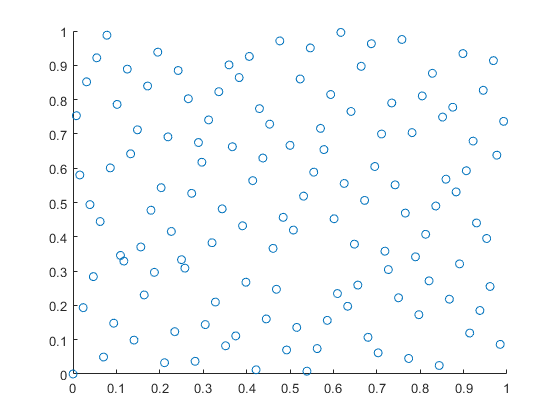
\includegraphics[scale=0.5]{images/halton_128.png}
	\caption{Los $128$ de la $Secuendia Halton (2,3)$ disponibles para usar.}\label{fig:halton128}
\end{figure}

El \textit{Anti-Aliasing} de Iluminación Especular, como en superficies metálicas, es un problema complejo en sí mismo, que requiere soluciones especializadas que funcionen directamente con los reflejos de la luz. Las técnicas \textit{Anti-Aliasing} no corrigen este problema por sí mismas, generalmente funcionan en conjunto con otras soluciones ya creadas. Para evitar problemas con la iluminación especular, se decidió apagarla.

Para probar las mejoras realizadas al \textit{Temporal Anti-Aliasing}, se agregaron los modelos de una esfera, pared, tubería, \textit{Hairball} (Bola de Pelo), una ventana con persianas y una ventana arqueada. Todos los modelos, excepto la pared, se agregaron con una textura de color sólido para evitar la introducción de errores de iluminación en los cálculos de las métricas de imagen, ya que estas son usadas para las comparaciones entre la implementación de Uncharted 4 y la desarrollada en este proyecto de grado. El modelo de la pared usa una textura blanca con letras negras, porque las letras usan bordes duros para definir su forma y debe permanecer así después de aplicar cualquier técnica de \textit{Anti-Aliasing}.

\subsection{Fast Approximate Anti-Aliasing (FXAA)}
Para este proyecto de grado, se usó la versión propuesta en el \textit{white paper} de \textit{Fast Approximate Anti-Aliasing} (FXAA, \textit{Anti-Aliasing} Aproximado Rápido) de Lottes \cite{Lottes2009}, para compararla con \textit{Temporal Anti-Aliasing}, basándose en que ambas técnicas son \textit{Anti-Aliasing} y post-procesamiento, y que FXAA es una técnica popular utilizada en la industria. Esta técnica se implementó con el ajuste de mayor calidad según el \textit{white paper}, sin considerar su impacto en el rendimiento, porque queríamos comparar la mejora cruda que ambas técnicas pueden proporcionar.

\subsection{Enhanced Subpixel Morphological Antialiasing (SMAA)}
Con la finalidad de probar una técnica de post-procesado más nueva y compleja, se implementó SMAA siguiendo las instrucciones proporcionadas por Jiménez et al \cite{Jimenez2012}. Se utilizó el valor preestablecido más alto que funciona con la Arquitectura de \textit{Shading} Diferido.

\subsection{Buffer de Acumulación}
Usamos un Buffer de Acumulación para proporcionar una imagen de referencia de la escena. Fue implementado siguiendo a Haeberli y Akeley \cite{Haeberli1990}. Los puntos usados para realizar \textit{jittering} a la cámara son los mismos puntos de la Secuencia de Halton que usa \textit{Temporal Anti-Aliasing}, aunque el Buffer de Acumulación puede usar hasta 128. Las razones para usar la Secuencia de Halton fueron: cumple con los requisitos establecidos por Haeberli y Akeley; es fácil ampliar el sistema de cámara actual para admitir más puntos Halton; e, igual que para \textit{Temporal Anti-Aliasing}, proporciona puntos pseudoaleatorios que no siguen un patrón para ayudar a reunir tanta información como sea posible de la escena.

\subsubsection{Número de Muestras Seleccionadas}
El número de muestras seleccionadas para el Buffer de Acumulación es 128. Esto se debe a que proporciona la mejor representación posible de la escena, a pesar de que causa una pérdida sustancial de rendimiento.

Para mostrar la diferencia entre el uso de 16 y 128 muestras, realizamos cuatro pruebas, identificadas de A a D, para observar cómo se comportan las medidas bajo diferentes arreglos de objetos e iluminación en la escena. En la tabla \ref{tab:acctest} vemos los resultados de una de esas pruebas:

\begin{table}[!hbt]
	\centering
	\caption{Comparación del comportamiento de las métricas entre el uso de 16 muestras frente a 128 para el Buffer de Acumulación.}\label{tab:acctest}
\begin{tabular}{  l  c  c  c  c  }
	\hline
	\multicolumn{5}{ c }{\textbf{Prueba D}} \\
	\hline
	\textbf{\diagbox{Pruebas}{Muestras}}  & \textbf{\makebox{16}} & \textbf{\makecell{128}} & \textbf{\makecell{Diferencia}} & \textbf{\makecell{Diferencia \\ Relativa (\%)}} \\
	\hline
	MSE de Temporal	& 40.6479 & 38.9473 & -1.7006 & 4.1837\% \\
	
	RMSD de Temporal & 6.3756 & 6.2408 & -0.1348 & 2.1142\% \\
	
	MSE de No AA & 24.8721 & 24.5250 & -0.3471 & 1.3956\% \\
	
	RMSD de No AA & 4.9872 & 4.9523 & -0.0349 & 0.7003\% \\
	
	Peak-SNR de Temporal & 32.0404 & 32.2260 & 0.1856 & 0.5759\% \\
	
	SNR de Temporal & 30.3060 & 30.4924 & 0.1864 & 0.6113\% \\
	
	Peak-SNR de No AA & 34.1737 & 34.2347 & 0.0610 & 0.1783\% \\
	
	SNR de No AA & 32.4392 & 32.5011 & 0.0618 & 0.1903\% \\
	
	SSIM de Temporal & 0.9933 & 0.9935 & 0.0001 & 0.0150\% \\
	
	SSIM de No AA & 0.9968 & 0.9969 & 0.0001 & 0.0065\% \\
	\hline		
\end{tabular}
\end{table}

En algunas métricas, los cambios son lo suficientemente grandes para ser perceptibles, especialmente en MSE y SSIM de Temporal Anti-Aliasing para nuestras comparaciones entre técnicas \textit{Anti-Aliasing}. Se pueden apreciar los efectos del uso de 128 muestras en el capítulo de comparaciones entre las técnicas \textit{Anti-Aliasing}.

\section{Implementación del Marco de Pruebas}
Para medir las mejoras logradas, desarrollamos un Marco de Pruebas que nos permite guardar la información importante cuando se realizan las pruebas. El marco nos permite seleccionar qué técnica utilizar como renderizador principal: \textit{Temporal Anti-Aliasing} implementado en el proyecto de grado, \textit{Temporal Anti-Aliasing} de \textit{Uncharted 4},  Enhanced Subpixel Morphological Anti-Aliasing (SMAA) o \textit{Fast Approximate Anti-Aliasing} (FXAA). También nos permite hacer \textit{zoom} en cualquier parte de la pantalla y luego realizar los cálculos de métricas de imágenes usando MATLAB.

Cuando se realiza una prueba, las imágenes renderizadas seleccionadas se guardan como  archivos PNG con 4 canales de color y sin compresión. Además, se guarda en un archivo de texto plano la información básica sobre la fecha en que se realizó la prueba, la información de la cámara y los datos de a los valores utilizados para el \textit{Temporal Anti-Aliasing}.

Para cuantificar si se lograron los objetivos propuestos de este proyecto de grado, sobre \textit{ghosting} y desenfoque, desarrollamos dos tipos diferentes de pruebas: Pruebas Estáticas y Pruebas de \textit{Ghosting}.

\subsection{Pruebas Estáticas}
Este tipo de prueba consiste en dejar que el Buffer de Historia se llene con 16 cuadros de la escena, sin ningún objeto en movimiento, utilizando la técnica \textit{Temporal Anti-Aliasing} seleccionada, para luego guardar el último cuadro renderizado. Inmediatamente después de guardar el último cuadro de TAA, renderizamos el último cuadro nuevamente pero ahora utilizando el Buffer de Acumulación, para generar la imagen base de la escena. También, renderizamos el último cuadro usando SMAA, FXAA y \textit{No Anti-Aliasing} (NOAA, No AA), para propósitos de comparación.

\subsection{Pruebas de Ghosting}
Este tipo de prueba  se ejecutó únicamente con los modelos de la Esfera y \textit{HairBall}, dado que son los únicos que nos interesa ver en movimiento y medir el \textit{Ghosting} que presentan. En el primero, la Esfera se mueve a través del pasillo de la escena, simulando un objeto en movimiento en una aplicación. En el segundo, el modelo de \textit{Hairball} gira en una posición estática, simulando muchos bordes en movimiento. La prueba consiste en renderizar la escena para un número seleccionado de cuadros, con la implementación del Proyecto de Grado de \textit{Temporal Anti-Aliasing} y la implementación de Uncharted 4 de \textit{Temporal Anti-Aliasing} al mismo tiempo. Después de renderizar cada cuadro, se guardan cada imagen, la posición de la esfera y la rotación de \textit{Hairball}

Una vez que el número seleccionado de cuadros se ha renderizado, la esfera se regresa a su posición original y el movimiento se repite utilizando las posiciones guardadas anteriormente. \textit{Hairball} también vuelve a su rotación original y el movimiento también se repite. La diferencia es que cada cuadro se procesa utilizando el Buffer de Acumulación y luego se guarda, se hace de esta forma para evitar la gran pérdida de rendimiento, que afecta las técnicas de \textit{Temporal Anti-Aliasing}.

Después de guardar todas las imágenes renderizadas, comparamos las producidas por el \textit{Temporal Anti-Aliasing} del Proyecto de Grado y el \textit{Temporal Anti-Aliasing} de Uncharted 4 contra la imagen base, generada con el Buffer de Acumulación, para calcular las métricas de imagen de ambos TAA. Estas métricas muestran cuánto error se generó por efecto de \textit{ghosting} en ambas implementaciones, lo que nos permite comparar el comportamiento de ambas técnicas. 


\subsection{Métricas de Imagen de MATLAB}
Las métricas de las imágenes para cada prueba representan, numéricamente, la calidad de cada imagen. Se calcularon para comparar cómo se comportó cada técnica en cada prueba, para identificar si el \textit{Temporal Anti-Aliasing} del Proyecto de Grado genera imágenes de mayor calidad que las otras técnicas probadas.

Una vez que se guardan los resultados de la prueba, una secuencia de comandos toma las imágenes y las organiza en carpetas por nombre y tipo de prueba. Después, los resultados de la prueba se procesan utilizando MATLAB, para obtener los resultados de las métricas de las imágenes. Con las métricas comparamos cómo se comportó el \textit{Temporal Anti-Aliasing} del Proyecto de Grado con el \textit{Temporal Anti-Aliasing} de Uncharted 4 y las otras técnicas \textit{Anti-Aliasing}, para detectar si las mejoras funcionaban y observar cómo se comporta nuestra implementación mejorada frente a las demás.

Para las Pruebas Estáticas, realizamos mediciones de MSE, RMSD, PSNR, SNR y SSIM en las imágenes renderizadas con TAA, FXAA, SMAA y No AA, utilizando las imágenes renderizadas del Buffer de Acumulación como referencia de comparación. Asimismo, generamos un mapa local de SSIM para cada imagen renderizada que es guardada, junto con renderizado con el Buffer de Acumulación (Imagen Base), como archivos PNG y FIG de MATLAB. Todos los resultados de las mediciones se almacenan en la carpeta con los resultados de la prueba como texto plano.

Para las Pruebas de Ghosting, realizamos mediciones de MSE, RMSD, PSNR, SNR y SSIM en cada cuadro procesado con la técnica de Temporal Anti-Aliasing de Uncharted 4 y la del Temporal Anti-Aliasing del Proyecto de Grado, utilizando el cuadro renderizado del Buffer de Acumulación correspondiente. Se generó un mapa local de SSIM para cada imagen renderizada, exceptuando las del Buffer de Acumulación, y se guardaron como  archivos  PNG y FIG de MATLAB. Los resultados de todas las imágenes se almacenaron en un archivo de texto plano. En los mapas locales de SSIM, las diferencias son representadas como colores, donde el blanco simboliza la similitud.


\section[Modificaciones de Temporal Reprojection Anti-Aliasing ]{Modificaciones de Temporal Reprojection Anti-Aliasing }
Para este proyecto de grado, la técnica del \textit{Color Clipping Box} se modificó para que se viera afectada por los valores calculados a partir de las nuevas técnicas aplicadas. Estos cambios siguen la lógica que queremos aplicar toda la fuerza de la técnica de \textit{Temporal Anti-Aliasing} únicamente cuando sea necesario y minimizar la aplicación de la técnica en otras partes, para minimizar los efectos de la \textit{ghosting} y desenfoque.

El primer cambio consiste en que los colores que se calcularon a partir del promedio entre las vecindades $3\times 3$ y Cruz, de los patrones de muestreo (ver Figura \ref{fig:samplingpattern_2}), se mezclan en una cantidad variable; a diferencia de antes donde solo se tomaba la el promedio entre ambos. El valor que utilizamos para mezclar se calcula en función de cuanto \textit{aliasing} consideramos que tiene el píxel siendo inspeccionado. La idea es que preferimos la vecindad de Cruz si el píxel que estamos calculando actualmente no se considera con \textit{aliasing}, porque es menos probable que la vecindad de Cruz introduzca ruido en los cálculos de la \textit{Color Clipping Box}. Pero, si se considera el píxel con \textit{aliasing}, preferimos el vecindario $3\times 3$ porque proporciona más información sobre el entorno del píxel para crear la imagen sin \textit{aliasing}. 

\begin{figure}[!hbt]
	\centering
	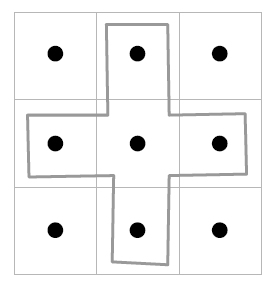
\includegraphics[scale=0.3]{images/sampling_pattern.png}
	\caption{Patrón de muestreo utilizado. Imagen tomada de la presentación de Fuglsand. \protect\cite{Fuglsand2016}}\label{fig:samplingpattern_2}
\end{figure}

El segundo cambio consiste en que el tamaño de la \textit{Color Clipping Box} depende de cuánto \textit{aliasing} se considera que tiene el píxel. Al utilizar \textit{Color Clipping Box} más pequeñas (Ver Figura \ref{fig:colorclippingboxredux}) que la técnica original en píxeles sin \textit{aliasing}, aumentamos la eliminación de colores no deseados del historial, reduciendo los efectos del \textit{Ghosting} ya que rechazamos colores más rápido en píxeles que sabemos que no se consideran con aliasing. Esto se implementa mediante la interpolación lineal del color de píxel actual y los colores mínimo y máximo calculados para construir la \textit{Color Clipping Box}.

\begin{figure}[!hbt]
	\centering
	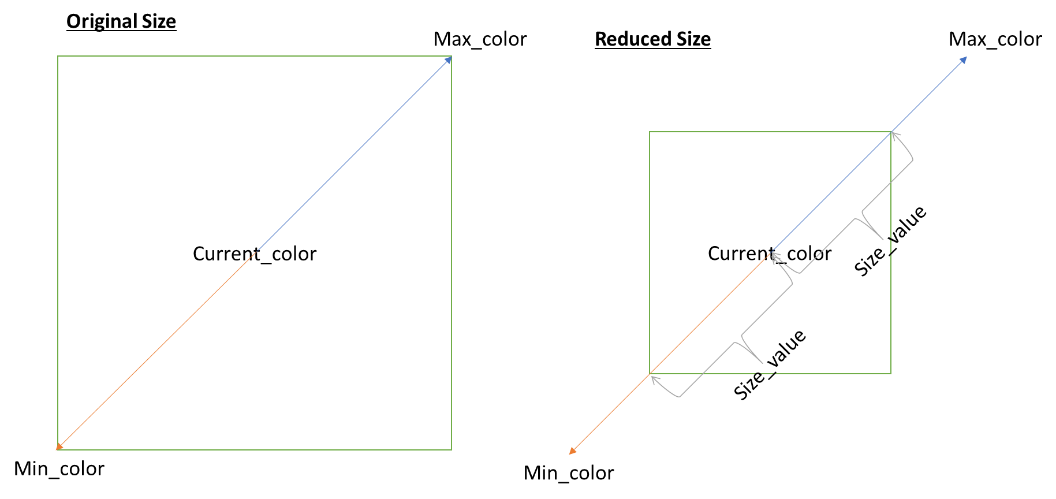
\includegraphics[scale=0.3]{images/clipping_box_reduction.png}
	\caption{Reducción de tamaño de la Color Clipping Box}\label{fig:colorclippingboxredux}
\end{figure}

En las siguientes secciones, explicaremos cómo se calculan los valores que contribuyen a decidir si un píxel se considera con \textit{aliasing} o no. Estos valores se calculan al mismo tiempo que se aplica TAA, con la excepción del Operador de Sobel, que ocurre antes de la técnica TAA principal. Más adelante mostraremos cómo usamos esos valores para reducir el tamaño del \textit{Color Clipping Box} y la preferencia del patrón de muestreo.

\subsection{Implementación de Mejoras de Indexación de Triángulos}
La idea principal detrás de la aplicación de esta técnica es detectar los píxeles que consideramos con \textit{aliasing}, utilizando la cantidad de modelos diferentes que rodean a un píxel. Queremos detectar los bordes entre diferentes modelos porque el \textit{aliasing} normalmente ocurre allí. Una vez que tenemos esta información, procedemos a modificar la \textit{Color Clipping Box} que controla la aplicación de TAA.

Para implementar esta técnica, todos los modelos en la escena reciben un índice único. Luego, en el pase de Renderización de Geometría, todos los triángulos que pertenecen a un mismo modelo reciben el índice del modelo como su identificación (ID). Posteriormente, se usa en el \textit{píxel shader} para generar una textura en la que cada píxel contiene el ID del modelo al que pertenece.

En el pase de Reproyección Temporal, se calcula el promedio del número de píxeles pertenecientes a diferentes modelos en la vecindad $3\times 3$ del píxel siendo revisado. Con este promedio, procedemos a sesgar la interpolación lineal de color entre el mínimo, máximo y promedio entre las vecindades Cruz y $3\times 3$ del píxel y procedemos a cambiar el tamaño del \textit{Color Clipping Box}.

Si el promedio es cercano a cero, lo que significa que el píxel está rodeado por píxeles de su mismo modelo, interpolamos hacia los colores de la vecindad Cruz y reducimos el tamaño de la \textit{Color Clipping Box}. Pero si el promedio es cercano a uno, lo que significa que el píxel está rodeado por muchos píxeles de otros modelos, interpolamos hacia los colores de la vecindad $3\times 3$ y dejamos que la \textit{Color Clipping Box} permanezca en su tamaño original.

\begin{equation}\label{eq:model_index_acc}
modelAverage_i = \frac{\sum\limits_{j=1}^{9} ModelDiff(i,j)}{9} 
\end{equation}

Donde
\begin{equation*}
ModelDiff(i,j) = \left\lbrace \begin{split}1\quad & if\quad ModelID_i \neq ModelID_j \\ 0\quad & else\end{split} \right.
\end{equation*}

A continuación, mostraremos algunos ejemplos de cómo funciona esta técnica. Para cada matriz, los números representan los ID de los triángulos, siendo la posición central el píxel que actualmente se está calculando y el resto su vecindad. La Matriz \ref{eq:triang_index_not_aliased} muestra un ejemplo de un píxel no considerado con \textit{aliasing} porque la mayoría de sus vecinos tienen el mismo ID. Por otro lado, la Matriz \ref{eq:triang_index_aliased} muestra un pixel considerado con \textit{aliasing} debido a la gran cantidad de ID diferentes alrededor.

\begin{equation}
\begin{bmatrix*}[r]\label{eq:triang_index_not_aliased}
3 &  3 & 3 \\
3 &  3 & 3 \\
5 &  23 & 82
\end{bmatrix*}
\end{equation}

\begin{equation}
\begin{bmatrix*}[r]\label{eq:triang_index_aliased}
3 &  3 & 3 \\
3 &  5 & 3 \\
5 &  23 & 82
\end{bmatrix*}
\end{equation}

\subsection{Pseudo-Varianza de Profundidad y Pseudo-Varianza Temporal de Profundidad}
La razón para utilizar esta técnica es que queremos detectar píxeles que están en una vecindad de píxeles separados por profundidades relativamente largas. También, queremos detectar píxeles cuya profundidad en el último cuadro cambió, relativamente, una distancia larga en contraste con su vecindad actual. Todos los píxeles que detectamos los consideramos con \textit{aliasing}.

Primero, calculamos la profundidad lineal mínima, máxima y su promedio del vecindario $3\times 3$. Luego procedemos a usar la siguiente fórmula para calcular el valor que utilizaremos para normalizar los resultados: 
\begin{equation} \label{eq:maxdepthdistance}
\begin{split} 
	maxDepthDistance = min \left( \right. & \left| depthMin-depthAvg \right|  ,   \\ 
	 &  \left.\left| depthMax-depthAvg\right| \right) 
\end{split} 
\end{equation}

Calculamos el valor de normalización utilizando el mínimo para evitar la interferencia de valores atípicos. Si $maxDepthDistance$ está por debajo de $0.002$, todo lo que sigue se establece en cero porque los píxeles están tan cerca que probablemente no tengan \textit{aliasing}. Este umbral se definió experimentando qué valores no generan ruido dentro de los cálculos, pero dejan entrar los píxeles interesantes.

Luego calculamos la Pseudo-Varianza de Profundidad como:

\begin{equation} \label{eq:depthpseudovariance}
	depthPseudoVariance = \left( \frac{\left|currentDepth-depthAvg\right|}{maxDepthDistance}\right)^2
\end{equation}

Esto nos proporciona una Pseudo-Varianza que mide la distancia entre la profundidad promedio de la vecindad y la profundidad actual del píxel. Hay que tener en cuenta que normalmente el valor va a estar entre $0$ y $1$ pero, si la profundidad del píxel es un valor atípico en la vecindad, este valor será superior a $1$.

Finalmente, calculamos cómo la profundidad del píxel en el último cuadro se relaciona con la vecindad actual, usando la Pseudo-Varianza Temporal de Profundidad. Hay que tener en cuenta que usamos la cuarta potencia para reducir el ruido en los cálculos. Dado que el valor normalizado está entre $0$ y $1$, el cálculo lo hace converger a $0$ si el valor es cercano a $0$ o a $1$ si es cercano a $1$.

\begin{equation} \label{eq:depthtemporalpseudovariance}
depthTemporalPseudoVariance = \left( \frac{\left|pastDepth-depthAvg\right|}{maxDepthDistance}\right)^4
\end{equation}

A continuación, mostraremos ejemplos de cómo esta técnica decide si un píxel se considera con \textit{aliasing} o no. Para cada matriz, los números representan las profundidades de los triángulos, siendo la posición central el píxel actual que se analiza y el resto es su vecindad. La Matriz \ref{eq:depth_var_not_aliased} nos muestra un ejemplo de un pixel no considerado con \textit{aliasing} porque está relativamente cerca de la mayoría de sus vecinos. Por otro lado, la Matriz \ref{eq:depth_var_aliased} muestra un ejemplo de un píxel que se consideraría con \textit{aliasing} porque tiene una distancia relativamente grande en comparación con su vecindad. Un ejemplo de un píxel considerado con \textit{aliasing} por la Pseudo-Varianza Temporal de Profundidad, sería si la profundidad del píxel de la Matriz \ref{eq:depth_var_not_aliased} en el último cuadro fuera de $4.0$.

\begin{equation}\label{eq:depth_var_not_aliased}
\begin{bmatrix*}[r]
9.0 &  9.3 & 8.7 \\
9.2 &  9.0 & 9.3 \\
8.8 &  8.9 & 8.7
\end{bmatrix*}
\end{equation}

\begin{equation}\label{eq:depth_var_aliased}
\begin{bmatrix*}[r]
9.0 &  9.3 & 8.7 \\
9.2 &  4.0 & 9.3 \\
8.8 &  8.9 & 8.7
\end{bmatrix*}
\end{equation}

\subsection{Implementación de las Mejoras de Sobel}
La idea principal detrás de la aplicación de la técnica de detección de bordes de Sobel es concentrar los efectos de aplicar TAA en los píxeles situados en los bordes, para corregir el \textit{aliasing}, en caso de ser necesario. Es importante señalar que esta es la única técnica de las mejoras del Proyecto de Grado que se ejecuta antes del algoritmo TAA principal.

Aplicamos el Operador Sobel a la luminancia de los colores de la escena iluminada producida por la Arquitectura de \textit{Shading} Diferido; la luminancia de los colores de la escena no iluminada del Buffer de Geometría; y la profundidad lineal actual. Utilizamos la luminancia porque el ojo humano reconoce mejor los cambios repentinos y usamos la escena, iluminada y no iluminada, para evitar problemas al detectar bordes debido a luces o sombras.

Cada operador de Sobel se ejecuta por separado y sus magnitudes se mezclan al final de la siguiente manera:
\begin{equation} \label{eq:sobel_g}
	g=(u*0.3 +l*0.7)+d 
\end{equation}

Donde $u$ es la magnitud del Operador Sobel de la luminancia de la escena no iluminada, $l$ es la magnitud del Operador Sobel de la luminancia de la escena iluminada y $d$ es la magnitud del Operador Sobel de la profundidad lineal actual. \\

Luego, restringimos(\textit{clamp}) $g$ entre $0.0$ y $1.0$ para finalmente aplicar el polinomio de paso suave (\textit{smoothstep}) de la siguiente manera:
\begin{equation} \label{eq:sobel_sqrt}
sobel=\sqrt{g^2*(3.0-2.0*g)} 
\end{equation}

Después de aplicar todos los Operadores de Sobel, guardamos los resultados en una textura y realizamos una versión simplificada de TRAA, para mantener los resultados estables a lo largo del tiempo. Esta versión simplificada es similar a la que usamos como base de este proyecto de grado, las diferencias provienen del uso de \textit{Clamping} (Restricción) en lugar de una \textit{Color Clipping Box}, porque los valores de textura son unidimensionales. Otra diferencia es que no aplicamos un Filtro de Nitidez.

La salida de este TRAA se usa para calcular el valor de Sobel del píxel actual, el valor promedio de Sobel en la Vecindad Cruz y el valor promedio de Sobel en la Vecindad $3\times 3$.

\subsection{Mezcla Final}
Finalmente, modificamos cómo se calcula la \textit{Color Clipping Box} utilizando los valores que calculamos previamente. Llamamos a este valor mezclado final $aliasedValue$, el cual representa la cantidad en que un píxel que se considera con \textit{aliasing}. Después de calcularlo, lo usamos para cambiar el patrón de muestreo a partir del cual se construye la \textit{Color Clipping Box} y su tamaño.

Primero, definimos la función de mezcla como:
\begin{equation} \label{eq:mixfunction}
Mix(x,y,t)=x*(1-t)+y*t\quad with\; 0\leq t\leq 1
\end{equation} 

Luego, la mezcla final se aplica de la siguiente manera:
\begin{equation}\label{eq:sobelavgmixval}
sobelAvgMixVal=Clamp01(modelAverage_i+sobel) 
\end{equation}
 
Donde $sobel$ es el valor Sobel del píxel actual, de la Ecuación \ref{eq:sobel_sqrt}, $modelAverage_i$ proviene de la Ecuación \ref{eq:model_index_acc} y $Clamp01$ es la función de Clamping (Restricción) entre $0$ y $1$. \\

\begin{equation}\label{eq:sobelavg}
sobelAvg=Mix(sobelAvgCross, sobelAvg3x3, sobelAvgMixVal)
\end{equation}

Donde $sobelAvgCross$ es el valor promedio de Sobel de la Vecindad Cruz y $sobelAvg3x3$ es el valor promedio de Sobel de la Vecindad $3\times 3$ alrededor del píxel actual. \\ 

Utilizamos las Ecuaciones \ref{eq:sobelavg}, \ref{eq:depthpseudovariance}, \ref{eq:depthtemporalpseudovariance} y \ref{eq:model_index_acc} para calcular cuánto \textit{aliasing} se considera que tiene este píxel:
\begin{equation}\label{eq:aliasedvalue}
\begin{split}
aliasedValue=Clamp01 (& sobelAvg + depthPseudoVariance \\
 & + depthTemporalPseudoVariance \\
 & + modelAverage_i)
\end{split}
\end{equation}

Con este $aliasedValue$ (valor de \textit{aliasing}) procedemos a modificar la \textit{Color Clipping Box}. Primero, seleccionamos cuánto de cada patrón de muestreo queremos que sea parte del \textit{Color Clipping Box}:
\begin{equation}\label{eq:newcolors}
\begin{split}
colorMin= & Mix(colorMinCross,colorMin3x3,aliasedValue) \\
colorMax= & Mix(colorMaxCross,colorMax3x3,aliasedValue) \\
colorAvg= & Mix(colorAvgCross,colorAvg3x3,aliasedValue) \\
\end{split}
\end{equation}

Luego modificamos el tamaño del \textit{Color Clipping Box} mediante la interpolación hacia el tamaño normal si el $aliasedValue$ está cerca de uno; en caso contrario, usamos el color actual, que es el centro del cuadro, lo cual disminuye el tamaño.
\begin{equation}\label{eq:clipredux}
\begin{split}
	clipColorMin= & Mix(colorCurrent,colorMin,aliasedValue) \\
	clipColorMax= & Mix(colorCurrent,colorMax,aliasedValue)
\end{split}
\end{equation}



Las Figuras \ref{fig:aliasedval1}, \ref{fig:aliasedval2} y \ref{fig:aliasedval3} son ejemplos de los valores de \textit{aliasing} calculados, cada píxel representa el $aliasedValue$ actual de esa imagen. El color blanco representa un $aliasedValue$ de $1$ y el color negro de $0$. Como esperamos, la mayoría de los bordes están marcados como probablemente con \textit{aliasing} por las técnicas utilizadas.

\begin{figure}[H]
	\centering
	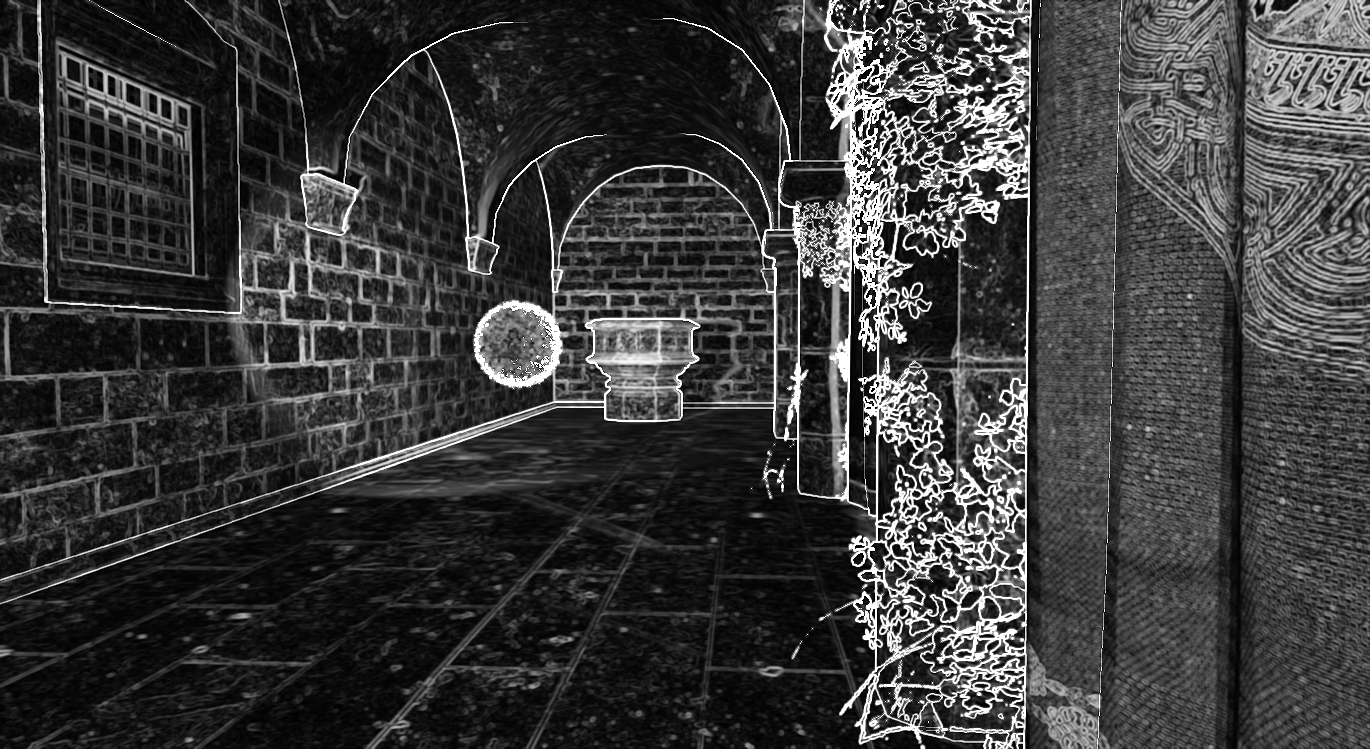
\includegraphics[scale=0.2]{images/aliased_value_example_1_temporal.png}
	\caption{Imagen hecha de los valores de \textit{aliasing} de cada píxel.}\label{fig:aliasedval1}
\end{figure}

\begin{figure}[H]
	\centering
	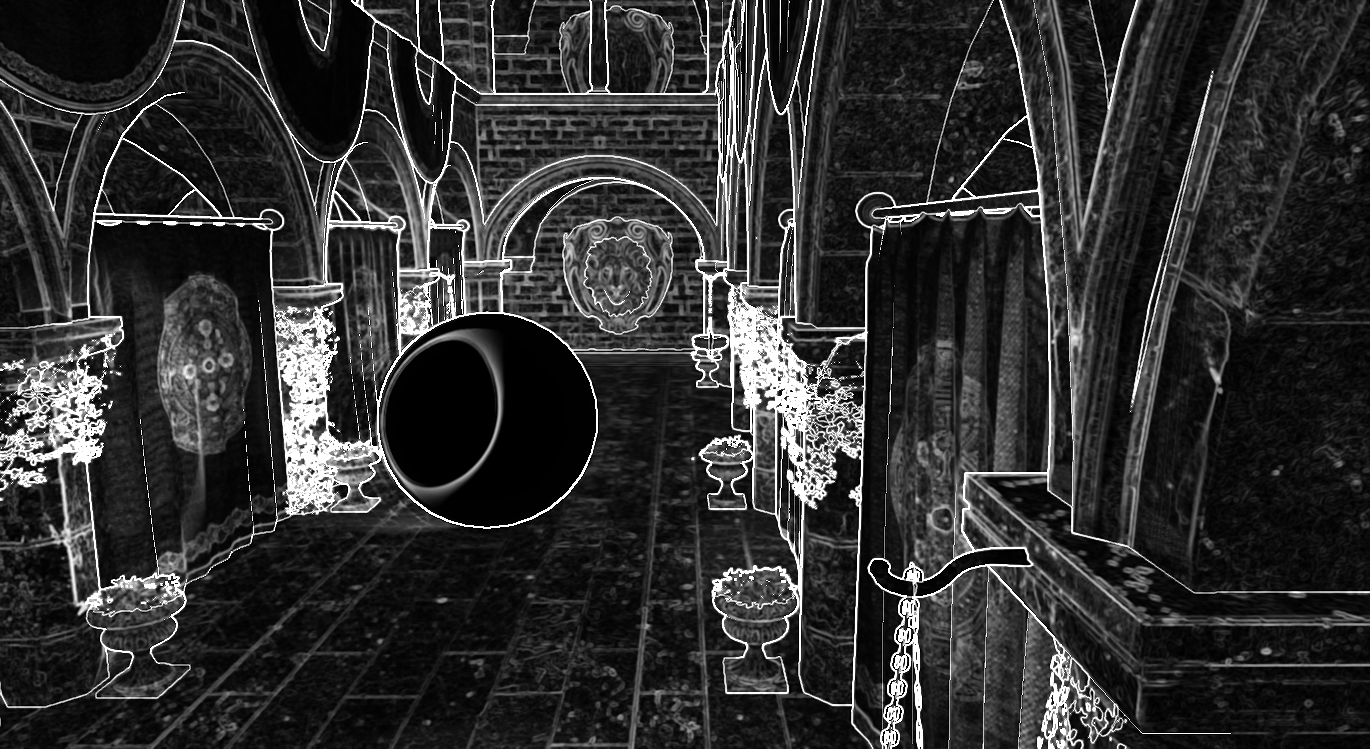
\includegraphics[scale=0.2]{images/aliased_value_example_2_temporal.png}
	\caption{Imagen hecha de los valores de \textit{aliasing} de cada píxel.}\label{fig:aliasedval2}
\end{figure}

\begin{figure}[H]
	\centering
	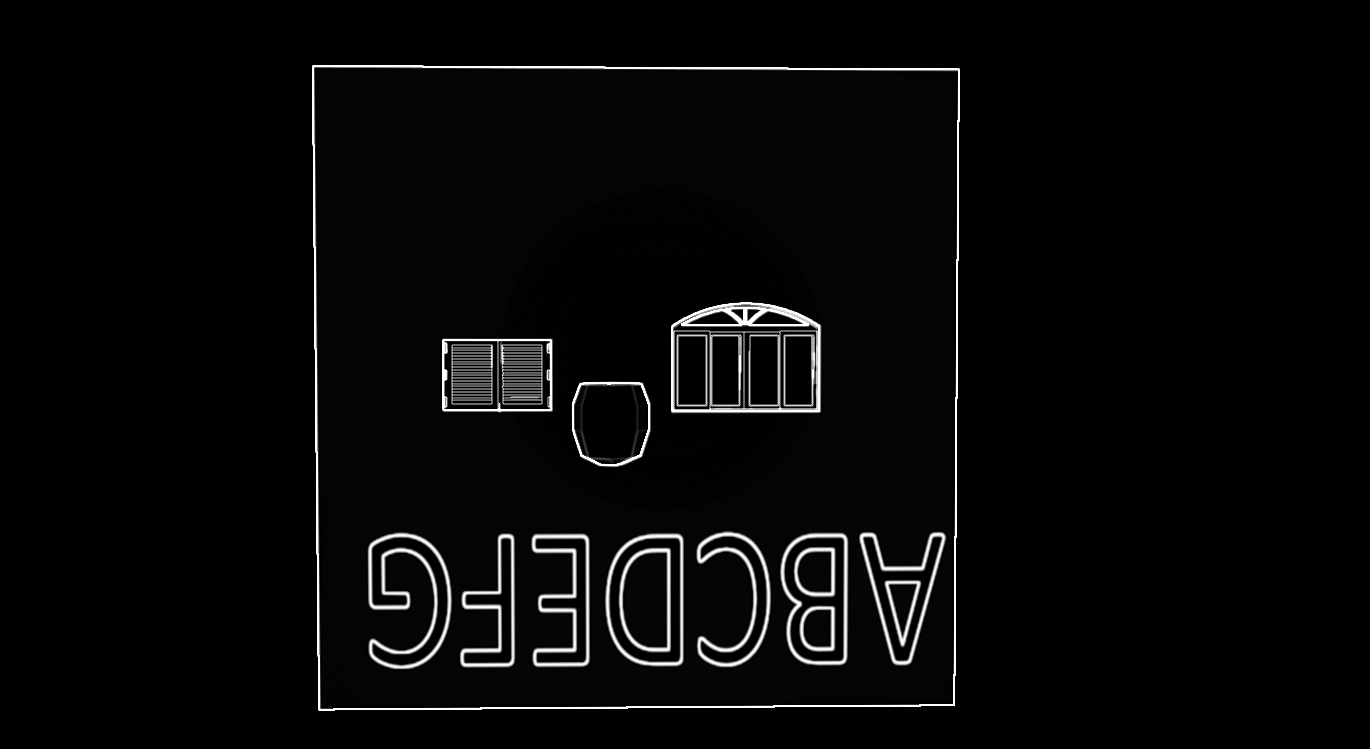
\includegraphics[scale=0.2]{images/aliased_value_example_3_temporal.png}
	\caption{Imagen hecha de los valores de \textit{aliasing} de cada píxel.}\label{fig:aliasedval3}
\end{figure}

\subsection{Modificaciones del Filtro de Nitidez}
Con el Filtro de Nitidez actual, se crea un pico de color cuando el píxel central es brillante y los píxeles vecinos están oscuros. Esto ocurre porque los colores oscuros son cercanos a cero y no son capaces de cancelar el aumento al píxel central, el cual se multiplica por $5$. Un ejemplo del peor caso posible es tener el píxel central con un color brillante y los píxeles del vecindario como negro puro, que se representan como cero. Por lo tanto, normalizamos el Filtro de Nitidez para evitar crear ese pico de color y trabajar mejor con píxeles brillantes en vecindarios oscuros. El filtro se cambió de \ref{eq:sharpen} a:
\begin{equation} \label{eq:new_sharpen}
\centering
\begin{bmatrix*}[c]
0 & -0.25 &  0 \\
-0.25  &  2 & -0.25  \\
0 & -0.25  &  0
\end{bmatrix*}
\end{equation}

La Ecuación \ref{eq:new_sharpen} muestra la nueva matriz de convolución del Filtro de Nitidez utilizada.


\chapter{Resultados}
En este capítulo, explicamos cómo evaluamos las mejoras realizadas al \textit{Temporal Anti-Aliasing}. Mostramos los resultados numéricos y visuales obtenidos. Finalmente, explicamos los resultados y su significado en comparación con la implementación anterior de TAA y otras soluciones de \textit{Anti-Aliasing}.

\section{Metodología de Evaluación}
Para evaluar las mejoras logradas en la técnica de \textit{Temporal Anti-Aliasing}, seleccionamos modelos y ángulos de cámara que colocan a la técnica bajo presión. Luego, utilizando el marco de prueba que desarrollamos, procedemos a renderizar y guardar imágenes de cada uno de esos modelos para comparar cómo se comporta la técnica en comparación con la implementación TAA original y otras técnicas \textit{Anti-Aliasing}, para determinar si las técnicas propuestas en este proyecto de grado proporcionan imágenes con mejor calidad sin incurrir en un uso excesivo de memoria o consumo de tiempo. Además, se realizó una prueba especial para medir si el cambio del Filtro de Nitidez era el único mecanismo que proporcionaba una mejora.

Los modelos utilizados en las pruebas fueron:
\begin{itemize}
\item Tubería: una tubería marrón con bordes duros.
\item Ventana con Persianas: una ventana azul con persianas cerradas.
\item Ventana Arqueada: una ventana azul con un arco en la parte superior.
\item Pared: una pared blanca con texto negro.
\item Atrium de Sponza: ejemplifica una escena general.
\item Flores del Atrium de Sponza: ejemplifica un modelo con recortes.
\item \textit{Hairball}: contiene muchos detalles finos por sus numerosas fibras.
\end{itemize}

Es importante tener en cuenta que en Computación Gráfica hay modelos comunes que se usan para probar técnicas, pero no existe un estándar per se. En este proyecto de grado, utilizamos dos modelos comunes: el Atrium de Sponza, que tiene muchas variaciones y se usa comúnmente para probar muchas técnicas de Computación Gráfica; y \textit{Hairball}, que a veces se usa para probar las técnicas \textit{Ray} y \textit{Path Tracing}. Para el resto de los modelos, presentamos una explicación del por qué se seleccionó cada uno en la sección correspondiente a cada una de las pruebas.

Los modelos del Atrium de Sponza y \textit{Hairball} se descargaron del \textit{Computer Graphics Archive} \cite{McGuire2017Data} de Morgan McGuire. El modelo de la Tubería es de Spencer Arts \cite{Spencer2010}. El modelo de Ventana Arqueada es de Isabela H. \cite{Isabela2016} y la Ventana con Persianas es de Channa Yim \cite{Channa2015}.

Las pruebas se realizaron en la computadora proporcionada por la Universidad de Lund, que tiene la siguiente especificación:
\begin{itemize}
\setlength\itemsep{0em}
\item CPU: Intel(R) Core(TM) i7-3820 CPU @ 3.60GHz, 3601 Mhz, 4 Cores, 8 Procesadores Lógicos
\item RAM: 64.0 GB	
\item GPU: NVIDIA GeForce GTX 1080 con 8 GB de VRAM
\item Resolución de Renderizado cuando no se utiliza el zoom: 1600 x 900
\end{itemize}

\section{Resultados y Comparaciones}
Para tener una base para analizar los datos, necesitamos observar que el mejor valor posible para MSE y RMSD es cero, lo que significa que no hay ningún error. Además, tener un alto valor de PSNR y SNR es mejor porque el ruido, que es el denominador en la ecuación de esta métrica, es cercano a cero. Finalmente, tener un SSIM de $1$ significa que la imagen es estructuralmente la misma que la imagen base, mientras que tener un valor de $0$ significa que es estructuralmente diferente. Para los mapas SSIM, cada píxel representa su valor SSIM. Tener un color blanco significa que es estructuralmente el mismo, mientras que tener un color más oscuro significa que hay diferencias estructurales.

\subsection{Filtro de Nitidez}
Para esta prueba, usamos el modelo del Atrium de Sponza y un modelo de una Esfera estática para evaluar los efectos del Filtro de Nitidez Normalizado en la calidad general de la imagen renderizada, especialmente con respecto al desenfoque causado normalmente por TAA. La escena fue seleccionada para esta prueba porque proporciona un ejemplo de una escena general, que no debería generar ningún efecto de desenfoque. Todo se procesó utilizando ambas implementaciones de TAA con y sin el Filtro de Nitidez Normalizado para observar si este cambio era la única mejora que aumentaba la calidad de la imagen procesada. Como se puede observar en la tabla \ref{tab:sharpen_res}, incluso cuando el TAA Mejorado del Proyecto de Grado y el TAA de Uncharted utilizan el Filtro de Nitidez Normalizado, las otras mejoras que hemos realizado  con el TAA renderiza una imagen de mayor calidad. Si hacemos zoom en la figura \ref{fig:sharpen_render} de la Figura \ref{fig:sharpen_ssim} podemos ver que el Filtro de Nitidez Normalizado contribuye a reducir los artefactos en la imagen renderizada, ya que casi no hay áreas oscuras en los mapas de SSIM de los TAA que lo está usando.

% Table generated by Excel2LaTeX from sheet 'Sharpen Filter'
\begin{table}[!htb]
	\small
	\centering
	\caption{Resultados numéricos de la prueba del Filtro de Nitidez}
	\begin{tabular}{m{5em} c c c c c}
		\hline
		\multicolumn{6}{c}{\textbf{Prueba del Filtro de Nitidez}} \\
		\hline
		\textbf{\makecell{\diagbox[innerwidth=5em]{Pruebas}{AA}}} & \textbf{\makecell{Uncharted \\ TAA \\ No \\ Normalizado}} & \textbf{\makecell{Uncharted \\ TAA \\ Normalizado}} & \textbf{\makecell{TAA \\ Mejorado \\ No \\ Normalizado}} & \textbf{\makecell{TAA \\ Mejorado \\ Normalizado}} & \textbf{\makecell{Mejor} } \\
		\hline
		MSE   & 149.271 & 8.835 & 148.036 & 8.224 & \textbf{\makecell{\scriptsize TAA \\ \scriptsize Mejorado \\ \scriptsize Normalizado}} \\
		
		RMSD  & 12.218 & 2.972 & 12.167 & 2.868 & \textbf{\makecell{\scriptsize TAA \\ \scriptsize Mejorado \\ \scriptsize Normalizado}} \\
		
		Peak-SNR  & 26.391 & 38.669 & 26.427 & 38.980 & \textbf{\makecell{\scriptsize TAA \\ \scriptsize Mejorado \\ \scriptsize Normalizado}} \\
		
		SNR   & 16.245 & 28.522 & 16.281 & 28.833 & \textbf{\makecell{\scriptsize TAA \\ \scriptsize Mejorado \\ \scriptsize Normalizado}} \\
		
		SSIM  & 0.932 & 0.992 & 0.933 & 0.992 & \textbf{\makecell{\scriptsize TAA \\ \scriptsize Mejorado \\ \scriptsize Normalizado}} \\
		\hline
	\end{tabular}%
	\label{tab:sharpen_res}%
\end{table}%

\begin{figure}[!htb]
	\centering
	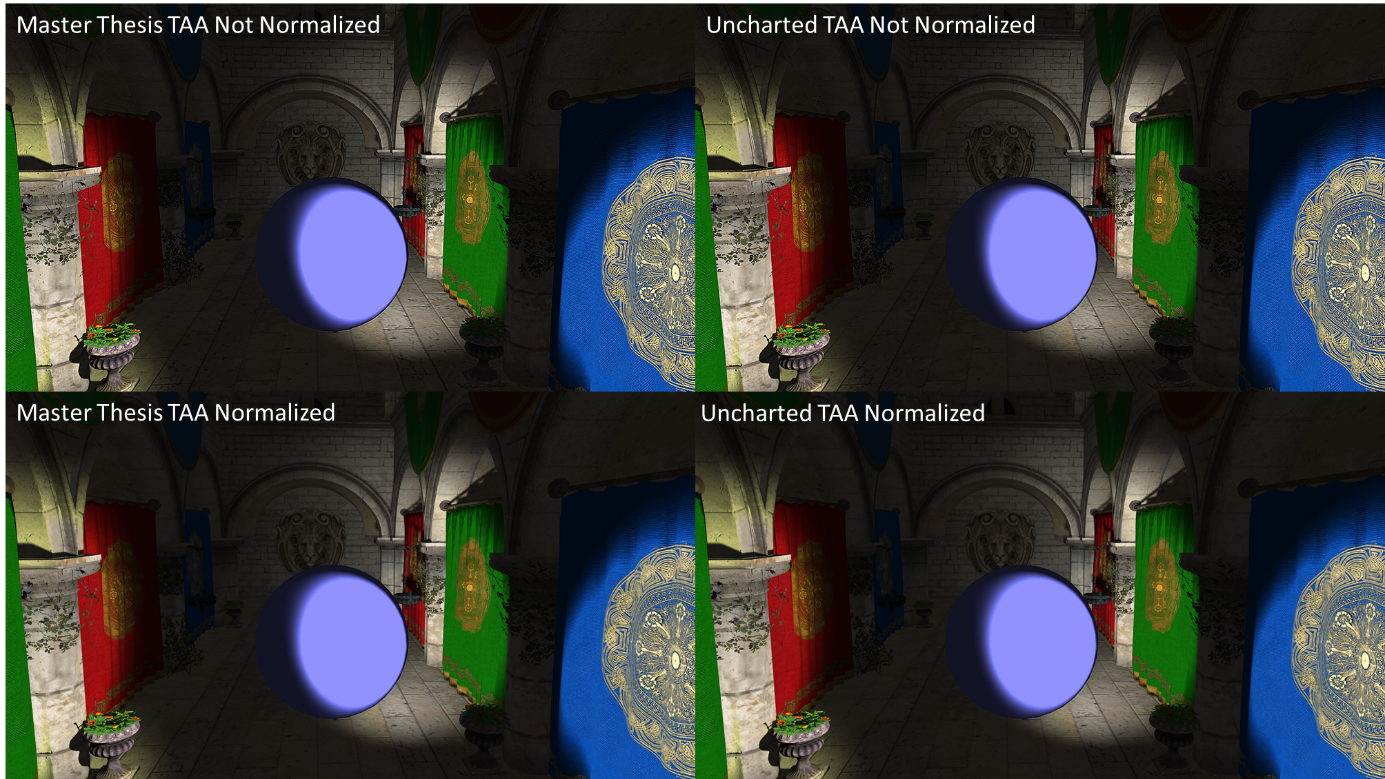
\includegraphics[scale=0.41]{images/results/sharpen_test_render.png}
	\caption{Comparación de las Imágenes Renderizadas.}\label{fig:sharpen_render}
\end{figure}

\begin{figure}[!htb]
	\centering
	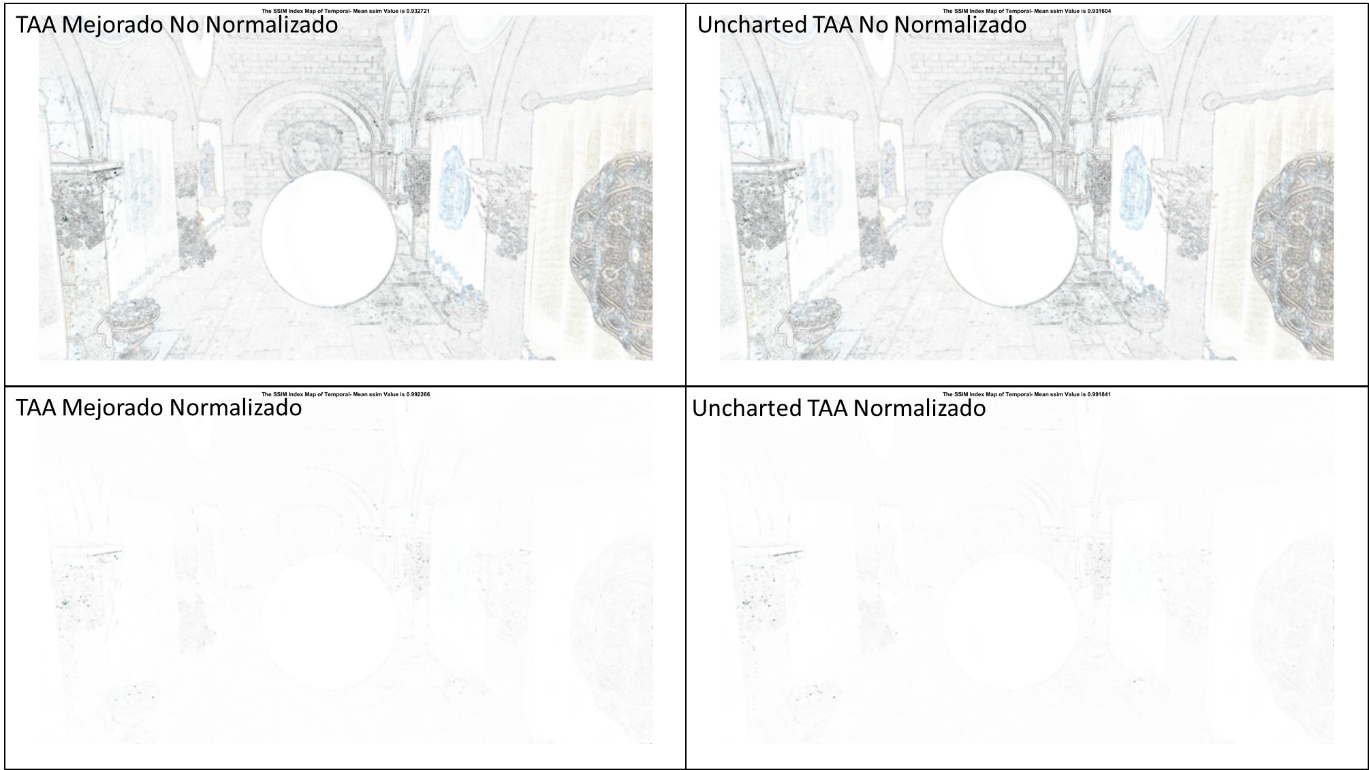
\includegraphics[scale=0.9]{images/results/sharpen_test_ssim.png}
	\caption{Comparación de Mapas de SSIM.}\label{fig:sharpen_ssim}
\end{figure}

\FloatBarrier
\subsection{Tubería}
Utilizamos el modelo de Tubería para probar cómo se comportan las mejoras al renderizar un modelo con bordes duros (\textit{hard edges}).  Queríamos probar si nuestras mejoras reducen la cantidad de desenfoque alrededor de esos bordes duros, mientras se disminuyen los problemas causados por el \textit{aliasing}. Renderizamos el tubo dos veces, la primera vez con un ángulo de cámara normal, para \textit{aliasing} normal alrededor de los bordes, y un ángulo de cámara inclinada, para aumentar los efectos de \textit{aliasing}. Como puede advertirse en los resultados, TAA con nuestras mejoras se encuentra en el mismo nivel de calidad que SMAA.

\subsubsection{Regular}
Cuando hacemos zoom y comparamos la Figura \ref{fig:pipe_regular_truth} con las imágenes renderizadas en la Figura \ref{fig:pipe_regular_render}, especialmente alrededor de los bordes, observamos que hay una reducción del desenfoque en el TAA del Proyecto de Grado en comparación con la TAA de Uncharted. Además, observamos que el TAA Uncharted genera colores brillantes alrededor de los bordes que no deberían estar; esto es más fácil de observar que los bordes oscuros en el Mapa de SSIM del TAA de Uncharted en la Figura \ref{fig:pipe_regular_render}. La Tabla \ref{tab:pipe_regular} nos confirma que el TAA del Proyecto de Grado alcanza casi la misma calidad que SMAA.

% Table generated by Excel2LaTeX from sheet 'Pipe Regular'
\begin{table}[!htb]	
	\small
	\centering
	\caption{Resultados numéricos de la prueba de Tubería con un ángulo de cámara regular.}
	\begin{tabular}{l c c c c c c c}
		\hline
		\multicolumn{8}{c}{\textbf{Prueba de Tubería Regular}} \\
		\hline
		\textbf{\diagbox[innerwidth=5em]{Pruebas}{AA}} & \textbf{No AA} & \textbf{FXAA}  & \textbf{SMAA}  & \textbf{\makecell{Uncharted \\ TAA}} & \textbf{\makecell{TAA \\ Mejorado}} & \textbf{Mejor} & \textbf{\makecell{TAA \\ Mejorado \\ Contra \\ El Mejor}} \\
		\hline
		MSE   & 8.608 & 3.573 & 1.278 & 14.602 & 1.574 & SMAA  & -0.296 \\
		
		RMSD  & 2.934 & 1.890 & 1.130 & 3.821 & 1.254 & SMAA  & -0.124 \\
		
		Peak-SNR  & 38.782 & 42.601 & 47.066 & 36.487 & 46.162 & SMAA  & 0.904 \\
		
		SNR   & 36.451 & 40.270 & 44.735 & 34.156 & 43.831 & SMAA  & 0.904 \\
		
		SSIM  & 0.999 & 0.999 & 1.000 & 0.996 & 1.000 & SMAA  & 0.000 \\
		\hline
	\end{tabular}%
	\label{tab:pipe_regular}%
\end{table}%

\begin{figure}[!htb]
	\centering
	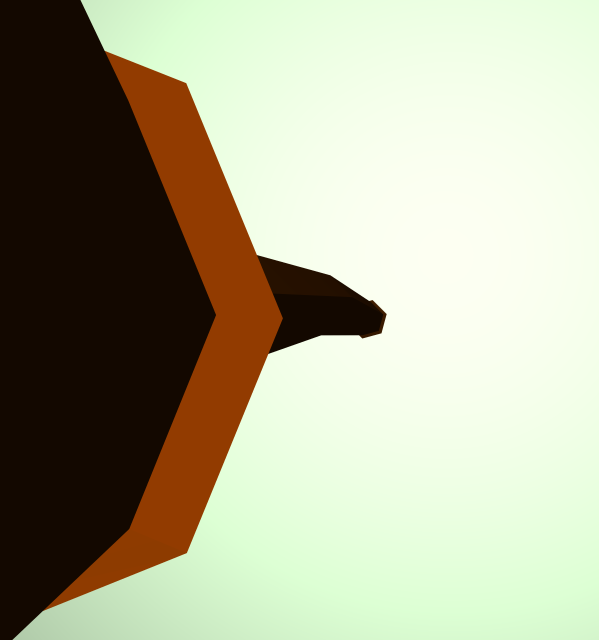
\includegraphics[scale=0.2]{images/results/pipe_regular_sobel_ground_truth.png}
	\caption{Imagen Base de la Prueba de Tubería Regular.}\label{fig:pipe_regular_truth}
\end{figure}


\begin{figure}[!htb]
	\centering
	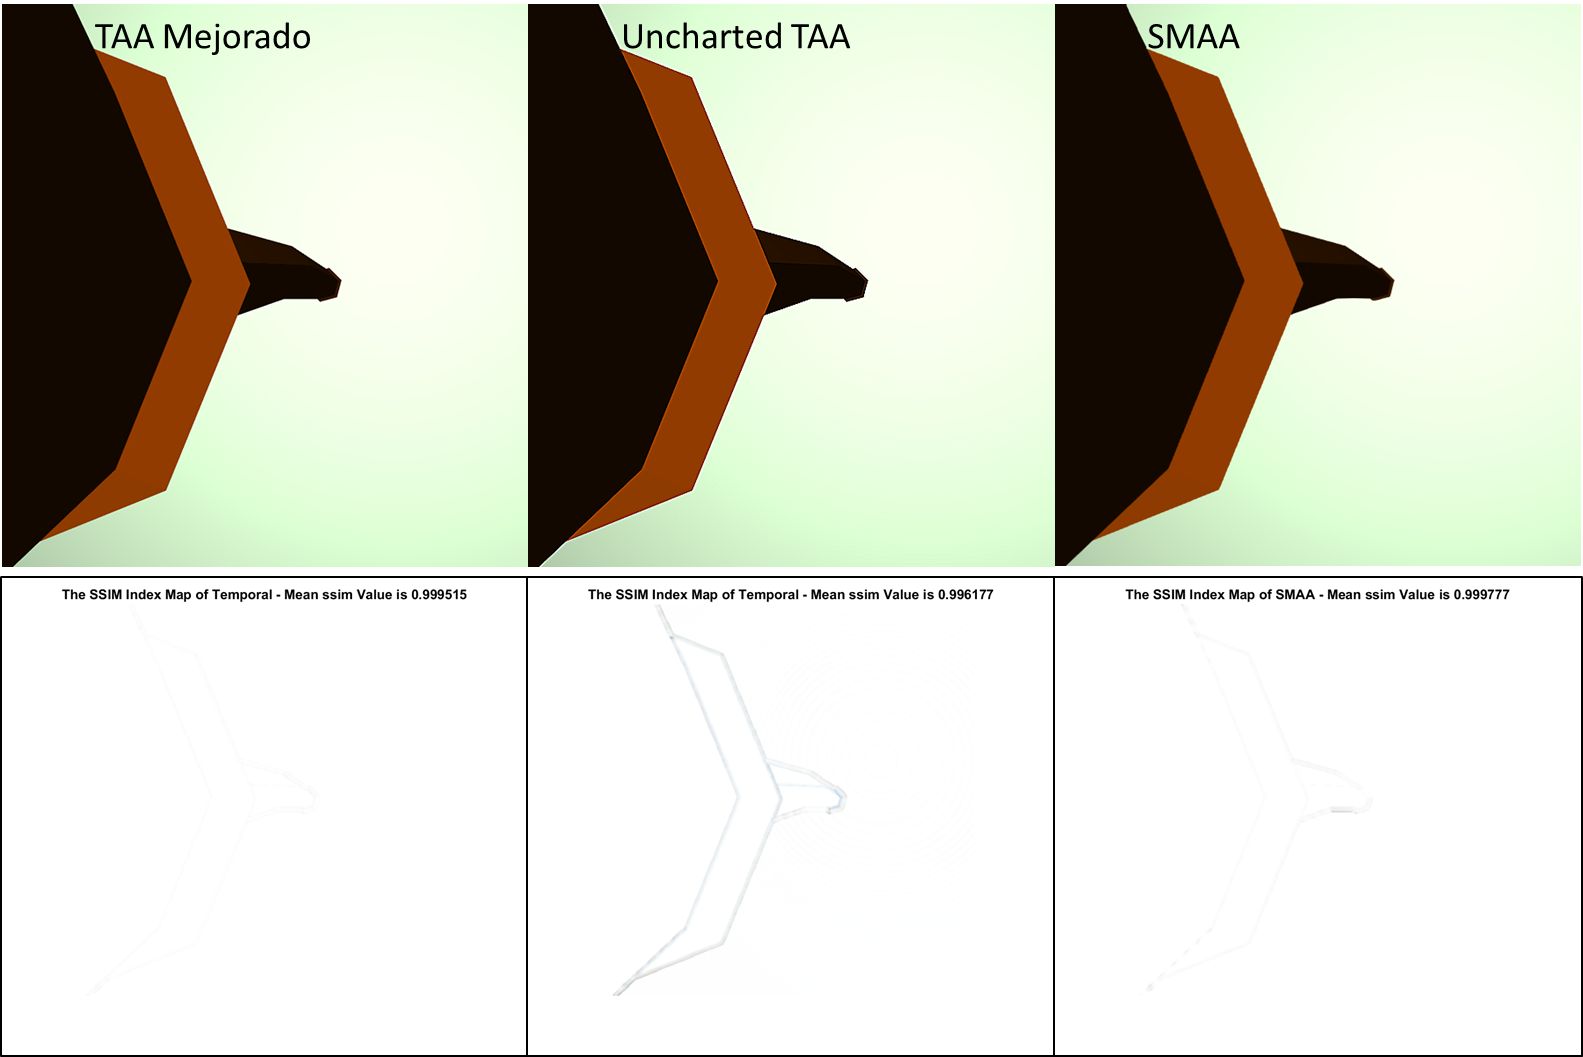
\includegraphics[scale=0.5]{images/results/pipe_regular.png}
	\caption{Comparación de Tubería Regular entre TAA del Proyecto de Grado, TAA de Uncharted y SMAA.}\label{fig:pipe_regular_render}
\end{figure}

\FloatBarrier

\subsubsection{Con Ángulo de Cámara Inclinada}
Al acercar y comparar las Figuras \ref{fig:pipe_inclination_render} y \ref{fig:pipe_inclination_truth}, podemos observar que el TAA Mejorado es el más semejante  a la imagen base. En el mapa de SSIM del TAA de Uncharted, notamos que se está generando desenfoque alrededor de los bordes.

Finalmente, en la Figura \ref{fig:pipe_inclination_render} y la Tabla \ref{fig:pipe_inclination_truth} observamos que SMAA no está detectando correctamente el borde superior de la tubería. Cuando hacemos zoom, notamos una pequeña escalera que se forma alrededor del borde. Esto se debe al hecho de que la cámara se configuró con una inclinación sesgada que llevó al límite las técnicas de detección de bordes utilizadas en SMAA.

% Table generated by Excel2LaTeX from sheet 'Pipe with Inclination'
\begin{table}[!htb]
	\small
	\centering
	\caption{Resultados numéricos de la prueba de Tubería con una inclinación de cámara sesgada.}
	\begin{tabular}{l c c c c c c c}
		\hline
		\multicolumn{8}{c}{\textbf{Prueba de Tubería con Inclinación de Cámara}} \\
		\hline
		\textbf{\diagbox[innerwidth=5em]{Pruebas}{AA}} & \textbf{No AA} & \textbf{FXAA}  & \textbf{SMAA}  & \textbf{\makecell{Uncharted \\ TAA}} & \textbf{\makecell{TAA \\ Mejorado}} & \textbf{Mejor} & \textbf{\makecell{TAA \\ Mejorado \\ Contra \\ El Mejor}} \\
		\hline
		MSE   & 16.112 & 6.470 & 2.810 & 14.349 & 2.664 & \makecell{TAA \\ Mejorado} & 0.000 \\
		
		RMSD  & 4.014 & 2.544 & 1.676 & 3.788 & 1.632 & \makecell{TAA \\ Mejorado} & 0.000 \\
		
		Peak-SNR  & 36.059 & 40.022 & 43.644 & 36.563 & 43.876 & \makecell{TAA \\ Mejorado} & 0.000 \\
		
		SNR   & 32.474 & 36.437 & 40.059 & 32.978 & 40.291 & \makecell{TAA \\ Mejorado} & 0.000 \\
		
		SSIM  & 0.998 & 0.999 & 1.000 & 0.996 & 0.999 & SMAA  & 0.000 \\
		\hline
	\end{tabular}%
	\label{tab:pipe_inclination}%
\end{table}%

\begin{figure}[!htb]
	\centering
	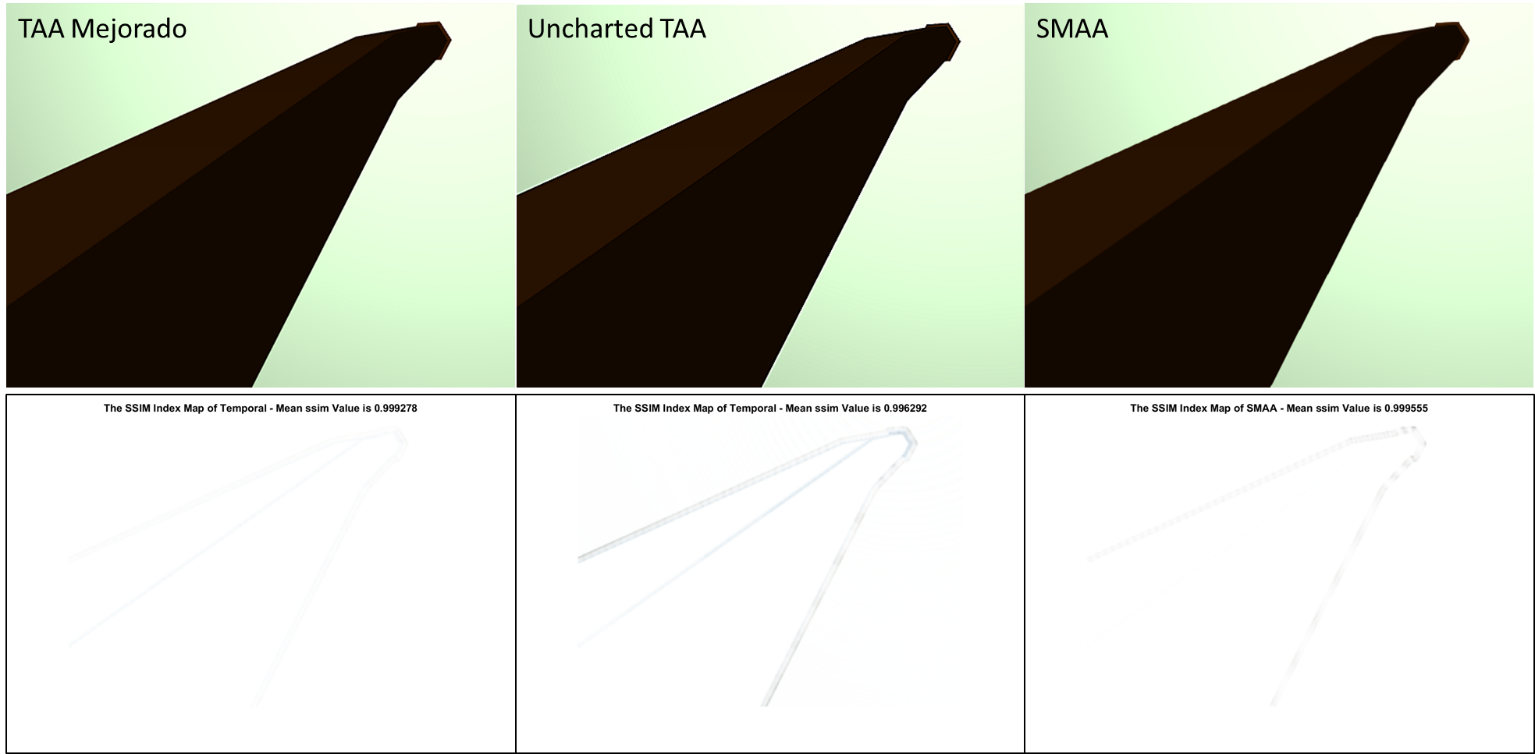
\includegraphics[scale=0.5]{images/results/pipe_inclination.png}
	\caption{Comparación de Prueba de Tubería con Inclinación de Cámara entre TAA del Proyecto de Grado, TAA de Uncharted y SMAA.}\label{fig:pipe_inclination_render}
\end{figure}

\begin{figure}[!htb]
	\centering
	
\includegraphics[scale=0.2]{images/results/pipe_with_inclination_sobel_ground_truth.png}
	\caption{Imagen Base de Prueba de Tubería con Inclinación de Cámara.}\label{fig:pipe_inclination_truth}
\end{figure}

\FloatBarrier

\subsection{Ventana con Persianas}
Usamos el modelo Ventana con Persianas por sus pequeños detalles en las persianas. Probamos cómo se comportan nuestras mejoras con este tipo de detalles y hallamos que visualmente no reacciona de manera adecuada, incluso si los resultados numéricos muestran lo contrario. 

En las Figuras \ref{fig:window_blind_render} y \ref{fig:window_blind_truth} podemos observar lo complicado que es para las técnicas manejar las pequeñas brechas entre las persianas. De la Figura \ref{fig:window_blind_render} y la Tabla \ref{tab:window_blind}, notamos que el TAA Mejorado y SMAA pueden reconstruir más detalles que el TAA de Uncharted pero, estética y visualmente, creemos que es mejor el TAA de Uncharted porque esos pequeños espacios entre las persianas parpadean menos, en comparación a las otras técnicas, cuando se mueve la cámara.

% Table generated by Excel2LaTeX from sheet 'Window Blind'
\begin{table}[!htb]
	\small
	\centering
	\caption{Resultados numéricos de la prueba de Ventana con Persianas.}
	\begin{tabular}{l c c c c c c c}
		\hline
		\multicolumn{8}{c}{\textbf{Prueba de Ventana con Persianas}} \\
		\hline
		\textbf{\diagbox[innerwidth=5em]{Pruebas}{AA}} & \textbf{No AA} & \textbf{FXAA}  & \textbf{SMAA}  & \textbf{\makecell{Uncharted \\ TAA}} & \textbf{\makecell{TAA \\ Mejorado}} & \textbf{Mejor} & \textbf{\makecell{TAA \\ Mejorado \\ Contra \\ El Mejor}} \\
		\hline
		MSE   & 96.044 & 70.486 & 35.134 & 170.229 & 32.115 & \makecell{TAA \\ Mejorado} & 0.000 \\
		
		RMSD  & 9.800 & 8.396 & 5.927 & 13.047 & 5.667 & \makecell{TAA \\ Mejorado} & 0.000 \\
		
		Peak-SNR  & 28.306 & 29.650 & 32.674 & 25.820 & 33.064 & \makecell{TAA \\ Mejorado} & 0.000 \\
		
		SNR   & 25.467 & 26.810 & 29.834 & 22.981 & 30.224 & \makecell{TAA \\ Mejorado} & 0.000 \\
		
		SSIM  & 0.986 & 0.990 & 0.995 & 0.976 & 0.995 & \makecell{TAA \\ Mejorado}  & 0.000 \\
		\hline
	\end{tabular}%
	\label{tab:window_blind}%
\end{table}%

\begin{figure}[!htb]
	\centering
	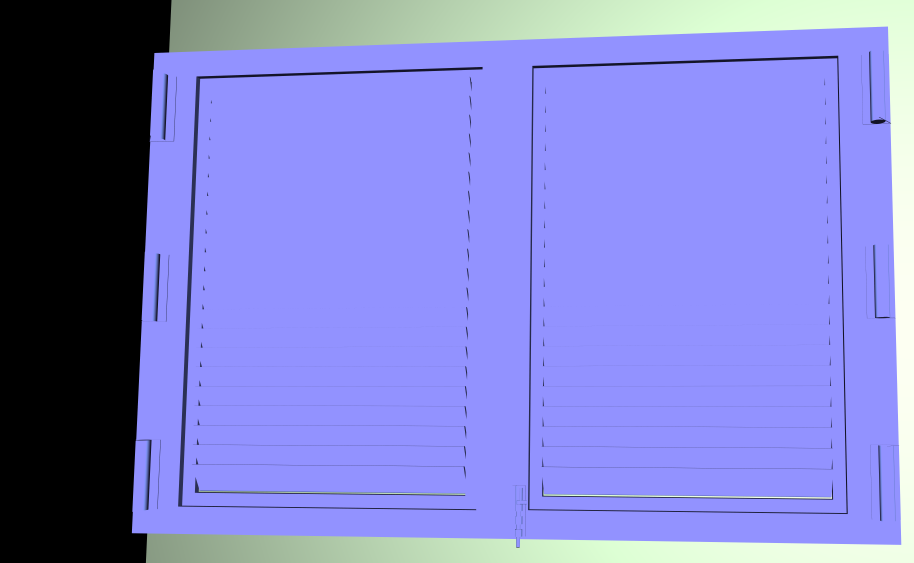
\includegraphics[scale=0.1]{images/results/window_blind_sobel_ground_truth.png}
	\caption{Imagen Base de Ventana con Persianas.}\label{fig:window_blind_truth}
\end{figure}

\begin{figure}[!htb]
	\centering
	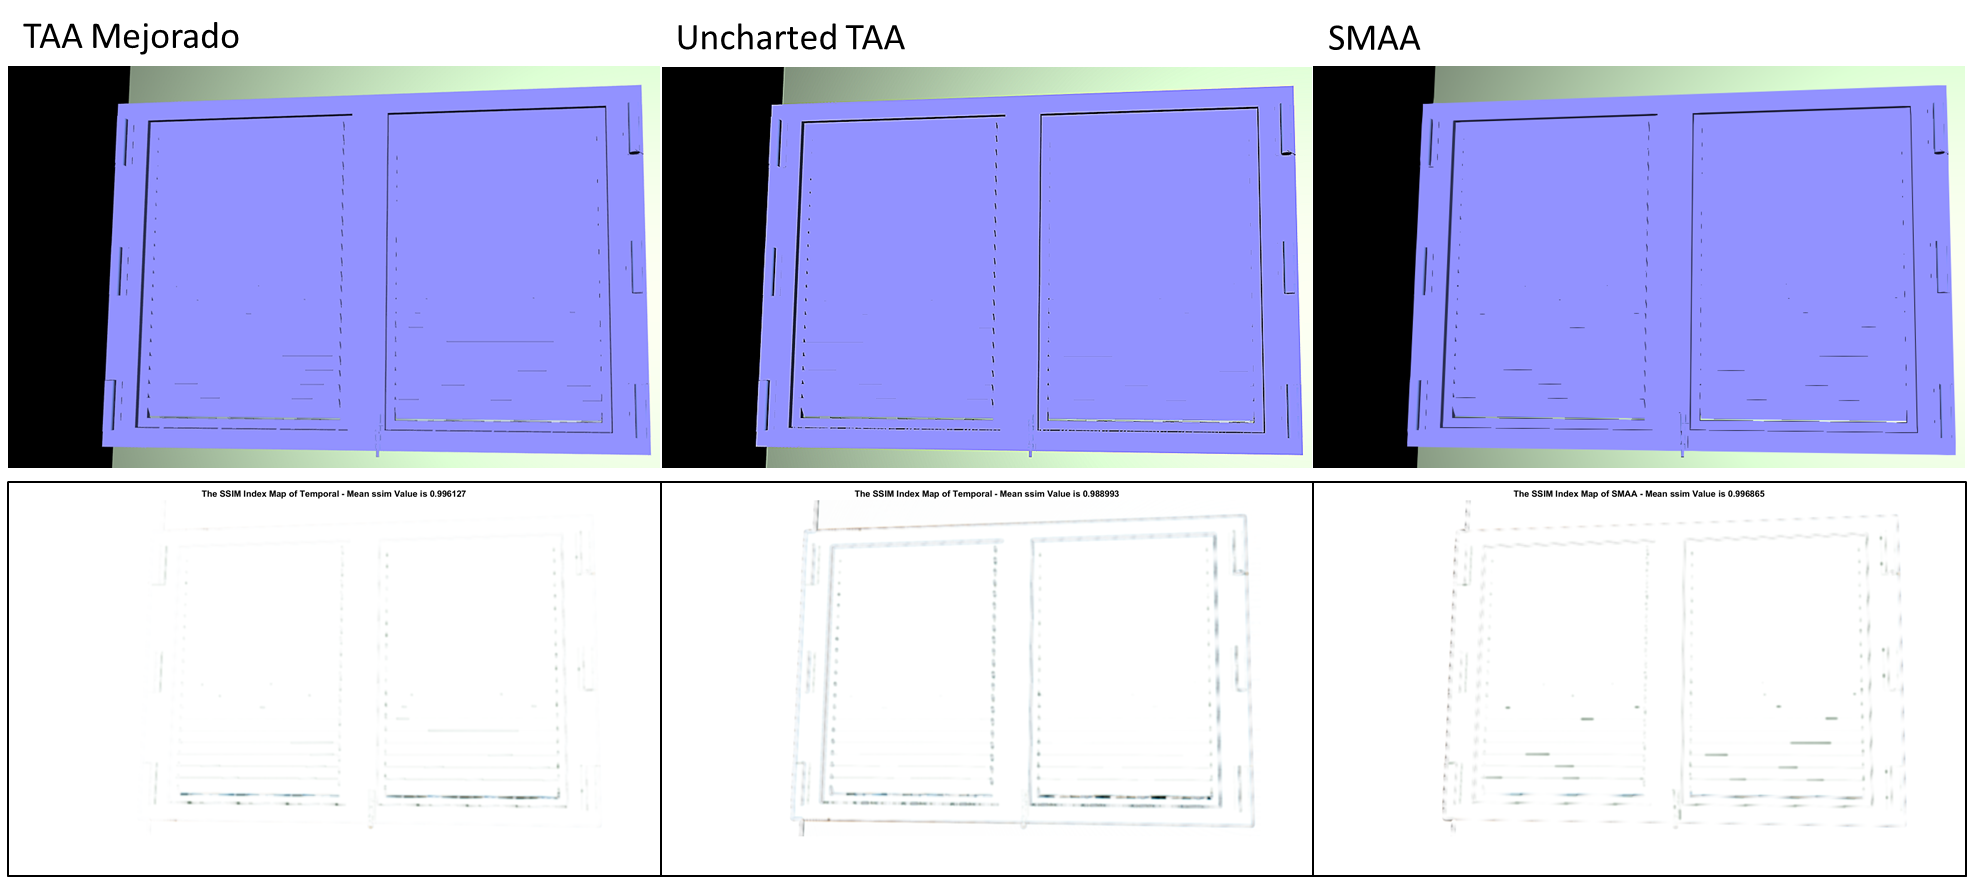
\includegraphics[scale=0.3]{images/results/window_blind.png}
	\caption{Comparación de Prueba de Ventana con Persianas entre TAA del Proyecto de Grado, TAA de Uncharted y SMAA.}\label{fig:window_blind_render}
\end{figure}

\FloatBarrier

\subsection{Ventana Arqueada}
Usamos el modelo de Ventana Arqueada para probar cómo nuestra implementación mejorada se comporta con los pequeños detalles de la puerta de la ventana y el \textit{aliasing} del arco. Podemos observar a partir de las Figuras \ref{fig:window_arch_render} y \ref{fig:window_arch_truth} que, para todas las técnicas, las pequeñas brechas alrededor de la ventana son difíciles de renderizar. En algunas partes de las brechas pequeñas, notamos que las técnicas no pueden renderizar la brecha por completo. Aunque en la Tabla \ref{tab:window_arch} SMAA parece ser el mejor, creemos que el TAA de Uncharted tiene la mejor calidad visual porque esos espacios incompletos generan menos parpadeos de píxeles cuando hay movimiento.
% Table generated by Excel2LaTeX from sheet 'Arched Window'
\begin{table}[!htb]
	\small
	\centering
	\caption{Resultados numéricos de la prueba de Ventana Arqueada.}
	\begin{tabular}{l c c c c c c c}
		\hline
		\multicolumn{8}{c}{\textbf{Prueba de Ventana Arqueada}} \\
		\hline
		\textbf{\diagbox[innerwidth=5em]{Pruebas}{AA}} & \textbf{No AA} & \textbf{FXAA}  & \textbf{SMAA}  & \textbf{\makecell{Uncharted \\ TAA}} & \textbf{\makecell{TAA \\ Mejorado}} & \textbf{Mejor} & \textbf{\makecell{TAA \\ Mejorado \\ Contra \\ El Mejor}} \\
		\hline
		MSE   & 56.313 & 39.103 & 19.849 & 76.483 & 21.983 & SMAA  & -2.134 \\
		
		RMSD  & 7.504 & 6.253 & 4.455 & 8.745 & 4.689 & SMAA  & -0.233 \\
		
		Peak-SNR  & 30.625 & 32.209 & 35.153 & 29.295 & 34.710 & SMAA  & 0.443 \\
		
		SNR   & 27.325 & 28.909 & 31.854 & 25.996 & 31.410 & SMAA  & 0.443 \\
		
		SSIM  & 0.992 & 0.994 & 0.997 & 0.989 & 0.996 & SMAA  & 0.001 \\
		\hline
	\end{tabular}%
	\label{tab:window_arch}%
\end{table}%

\begin{figure}[!htb]
	\centering
	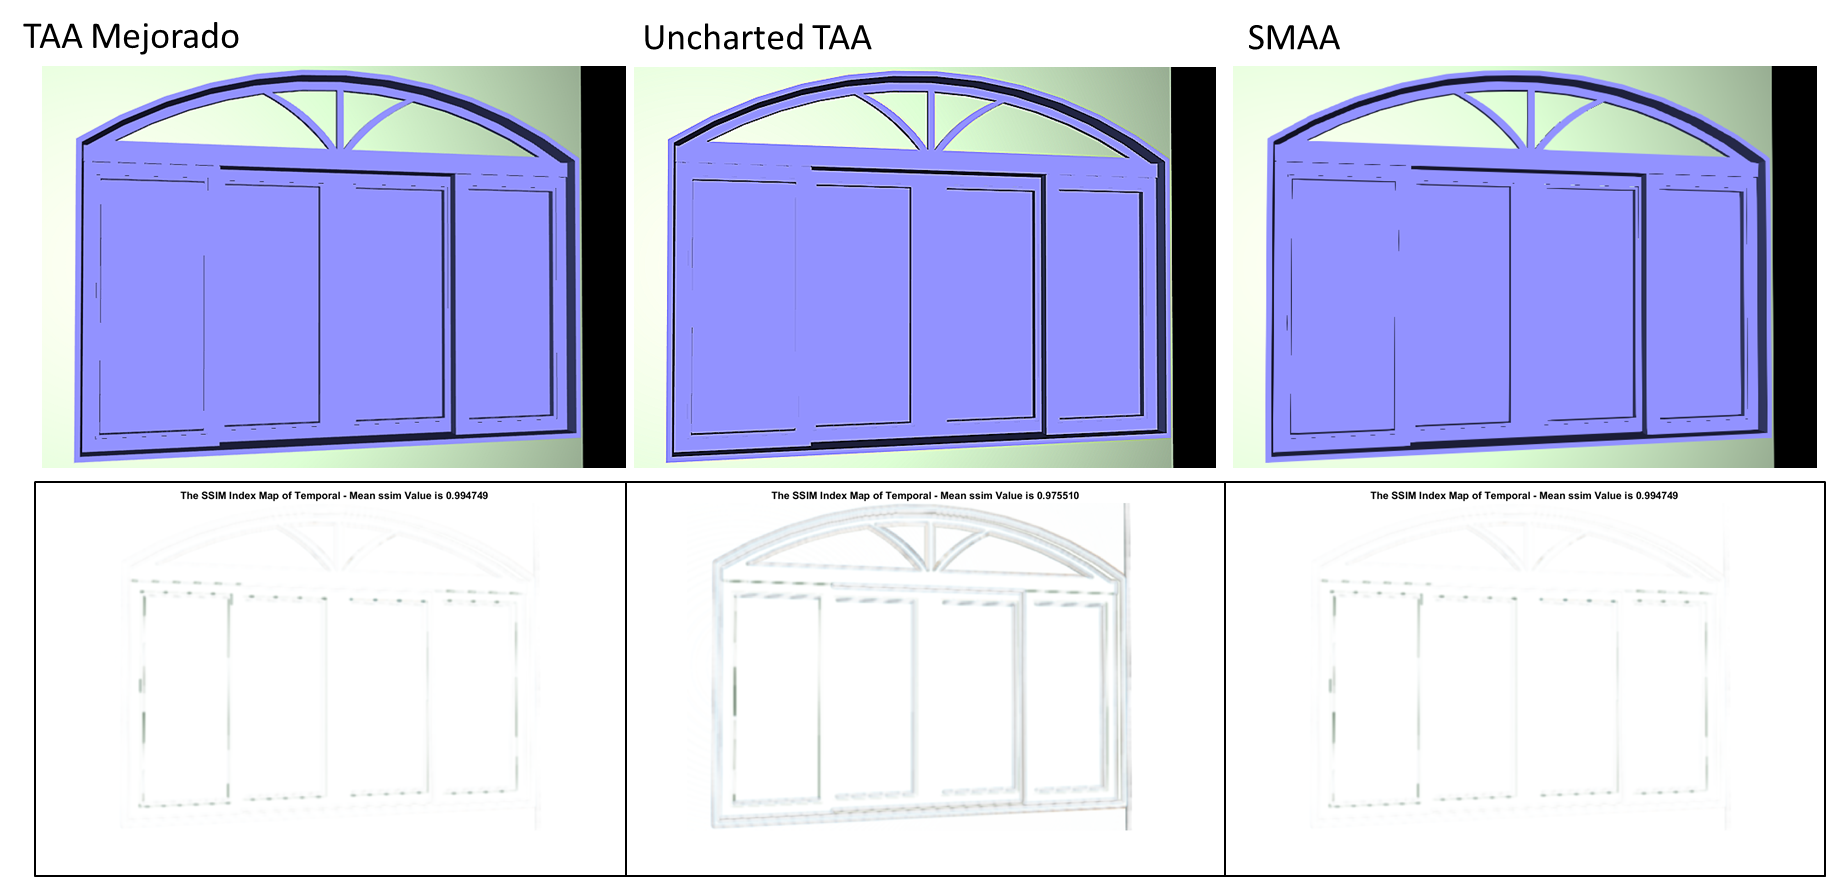
\includegraphics[scale=0.3]{images/results/window_arch.png}
	\caption{Comparación de Prueba de Ventana Arqueada entre TAA del Proyecto de Grado, TAA de Uncharted y SMAA.}\label{fig:window_arch_render}
\end{figure}

\begin{figure}[!htb]
	\centering
	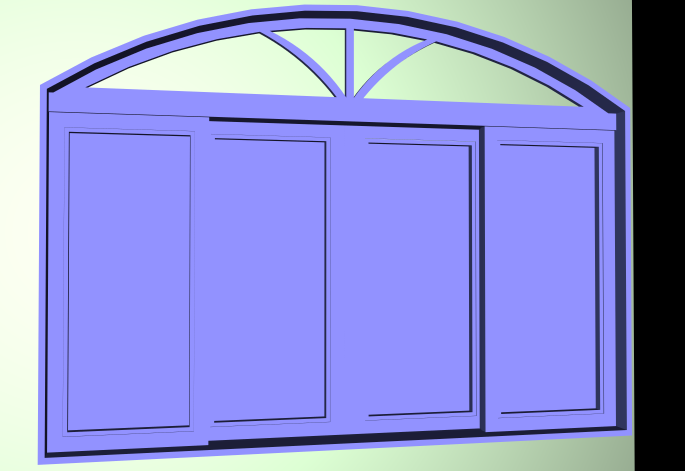
\includegraphics[scale=0.18]{images/results/window_arch_sobel_ground_truth.png}
	\caption{Imagen Base de Ventana Arqueada.}\label{fig:window_arch_truth}
\end{figure}

\FloatBarrier

\subsection{Atrium de Sponza}
Con esta prueba queremos analizar cómo se comporta la implementación de TAA del Proyecto de Grado con una escena general con luces y sombras. Utilizamos el modelo del Atrium de Sponza con el modelo de Esfera estática en el centro.

Si comparamos las Figuras \ref{fig:sponza_render} y \ref{fig:sponza_truth}, podemos observar que el TAA de Uncharted tiene problemas de desenfoque alrededor de todos los bordes, esto es visible en su Mapa de SSIM. SMAA tuvo problemas con todas las flores, podemos observar la forma de las flores en su Mapa de SSIM. El TAA Mejorado solo tiene problemas menores con las flores, como se ve en las áreas grises en su Mapa de SSIM. La Tabla \ref{tab:sponza} confirma lo que estamos observando en los resultados visuales, ya que el TAA Mejorado del Proyecto de Grado obtuvo los mejores resultados en la mayor parte de la prueba; mientras que el TAA de Uncharted obtuvo las peores resultados debido a los problemas de bordes; y SMAA empeoró debido al problema de las flores.
% Table generated by Excel2LaTeX from sheet 'Sponza Table'
\begin{table}[!htb]
	\small
	\centering
	\caption{Resultados numéricos de la Prueba del Atrium de Sponza.}
	\begin{tabular}{l c c c c c c c}
		\hline
		\multicolumn{8}{c}{\textbf{Prueba del Atrium de Sponza}} \\
		\hline
		\textbf{\diagbox[innerwidth=5em]{Pruebas}{AA}} & \textbf{No AA} & \textbf{FXAA}  & \textbf{SMAA}  & \textbf{\makecell{Uncharted \\ TAA}} & \textbf{\makecell{TAA \\ Mejorado}} & \textbf{Mejor} & \textbf{\makecell{TAA \\ Mejorado \\ Contra \\ El Mejor}} \\
		\hline
		MSE   & 13.458 & 8.290 & 8.610 & 42.728 & 3.972 & \makecell{TAA \\ Mejorado} & 0.000 \\
		
		RMSD  & 3.669 & 2.879 & 2.934 & 6.537 & 1.993 & \makecell{TAA \\ Mejorado} & 0.000 \\
		
		Peak-SNR  & 36.841 & 38.945 & 38.781 & 31.824 & 42.141 & \makecell{TAA \\ Mejorado} & 0.000 \\
		
		SNR   & 20.056 & 22.160 & 21.996 & 15.038 & 25.356 & \makecell{TAA \\ Mejorado} & 0.000 \\
		
		SSIM  & 0.988 & 0.991 & 0.991 & 0.938 & 0.991 & \makecell{TAA \\ Mejorado}  & 0.000 \\
		\hline
	\end{tabular}%
	\label{tab:sponza}%
\end{table}%

\begin{figure}[!htb]
	\centering
	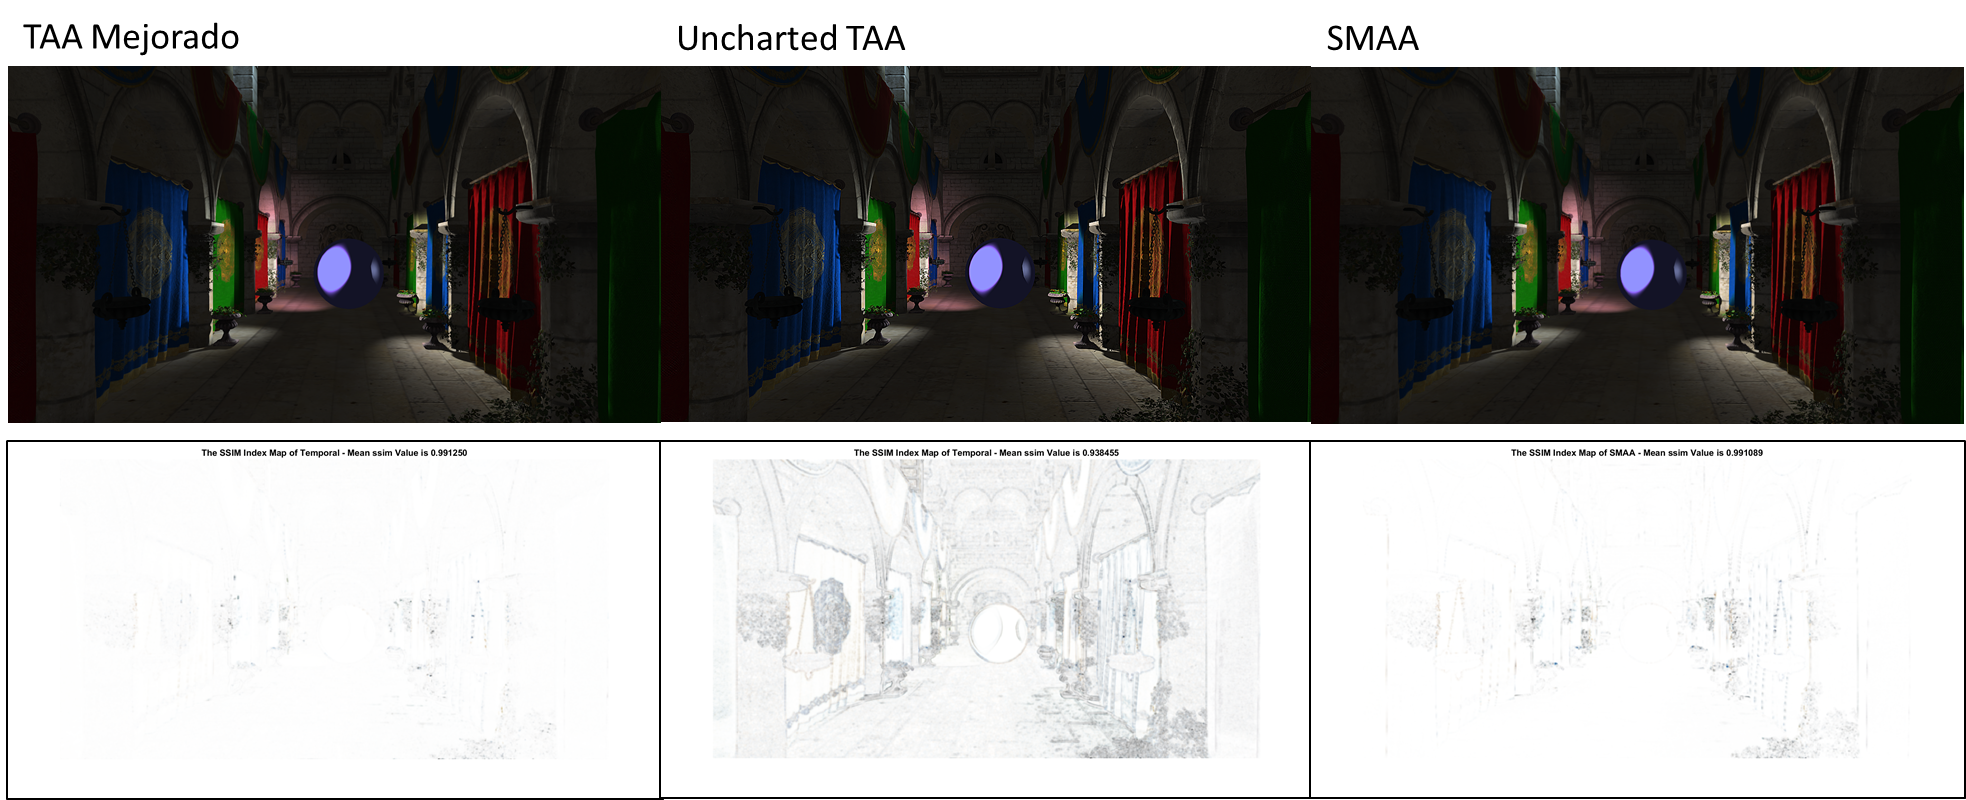
\includegraphics[scale=0.3]{images/results/sponza.png}
	\caption{Comparación de Prueba del Atrium de Sponza entre TAA del Proyecto de Grado, TAA de Uncharted y SMAA.}\label{fig:sponza_render}
\end{figure}

\begin{figure}[!htb]
	\centering
	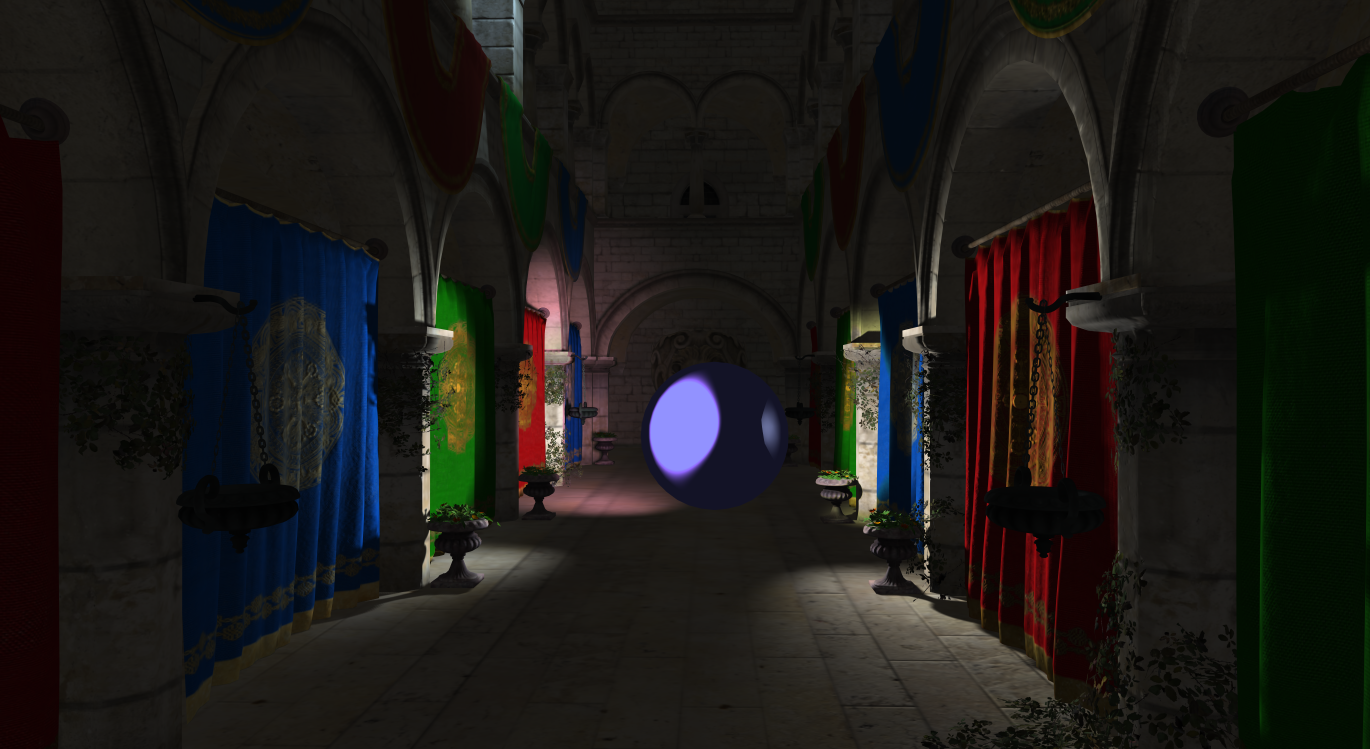
\includegraphics[scale=0.1]{images/results/sponza_sobel_ground_truth.png}
	\caption{Imagen Base del Atrium de Sponza.}\label{fig:sponza_truth}
\end{figure}

\FloatBarrier

\subsection{Flores del Atrium de Sponza}
En esta prueba vimos cómo nuestras mejoras manejan los detalles de un modelo con partes transparentes, como son las flores del modelo del Atrium de Sponza. El \textit{aliasing} que presentan este tipo de modelos se considera difícil de detectar y corregir correctamente. 

En las Figuras \ref{fig:sponza_flowers_render} y \ref{fig:sponza_flowers_truth}, notamos que el TAA de Uncharted tiene problemas para manejar este tipo de modelo, especialmente si observamos su Mapa de SSIM. Notamos que SMAA no pudo corregir todos los artefactos de aliasing de los bordes de las flores, vemos que la silueta de las flores aparece en su Mapa de SSIM.  Finalmente, observamos que el TAA del Proyecto de Grado corrigió la mayoría de los artefactos de aliasing, aunque algunos todavía aparecen como áreas grises en su Mapa de SSIM. Además, la Tabla \ref{tab:sponza_flowers} confirma lo que percibimos visualmente, ya que el TAA del Proyecto de Grado obtuvo los mejores puntajes y SMAA obtuvo una puntuación peor que el promedio.

% Table generated by Excel2LaTeX from sheet 'Sponza Flowers'
\begin{table}[!htb]
	\small
	\centering
	\caption{Resultados numéricos de la Prueba de las Flores del Atrium de Sponza.}
	\begin{tabular}{l c c c c c c c}
		\hline
		\multicolumn{8}{c}{\textbf{Prueba de las Flores del Atrium de Sponza}} \\
		\hline
		\textbf{\diagbox[innerwidth=5em]{Pruebas}{AA}} & \textbf{No AA} & \textbf{FXAA}  & \textbf{SMAA}  & \textbf{\makecell{Uncharted \\ TAA}} & \textbf{\makecell{TAA \\ Mejorado}} & \textbf{Mejor} & \textbf{\makecell{TAA \\ Mejorado \\ Contra \\ El Mejor}} \\
		\hline
		MSE   & 122.795 & 66.062 & 72.279 & 490.281 & 36.162 & \makecell{TAA \\ Mejorado} & 0.000 \\
		
		RMSD  & 11.081 & 8.128 & 8.502 & 22.142 & 6.013 & \makecell{TAA \\ Mejorado} & 0.000 \\
		
		Peak-SNR  & 27.239 & 29.931 & 29.541 & 21.226 & 32.548 & \makecell{TAA \\ Mejorado} & 0.000 \\
		
		SNR   & 19.590 & 22.282 & 21.891 & 13.577 & 24.899 & \makecell{TAA \\ Mejorado} & 0.000 \\
		
		SSIM  & 0.959 & 0.975 & 0.972 & 0.863 & 0.985 & \makecell{TAA \\ Mejorado} & 0.000 \\
		\hline
	\end{tabular}%
	\label{tab:sponza_flowers}%
\end{table}%

\begin{figure}[!htb]
	\centering
	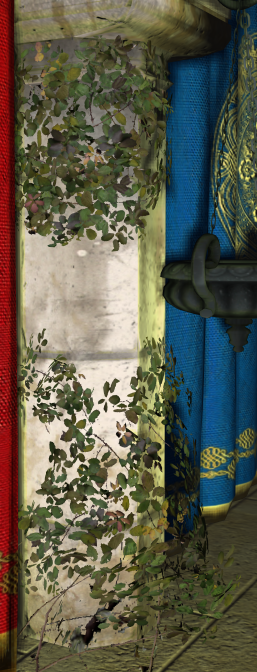
\includegraphics[scale=0.2]{images/results/sponza_flowers_sobel_ground_truth.png}
	\caption{Imagen Base de las Flores del Atrium de Sponza.}\label{fig:sponza_flowers_truth}
\end{figure}

\begin{figure}[!htb]
	\centering
	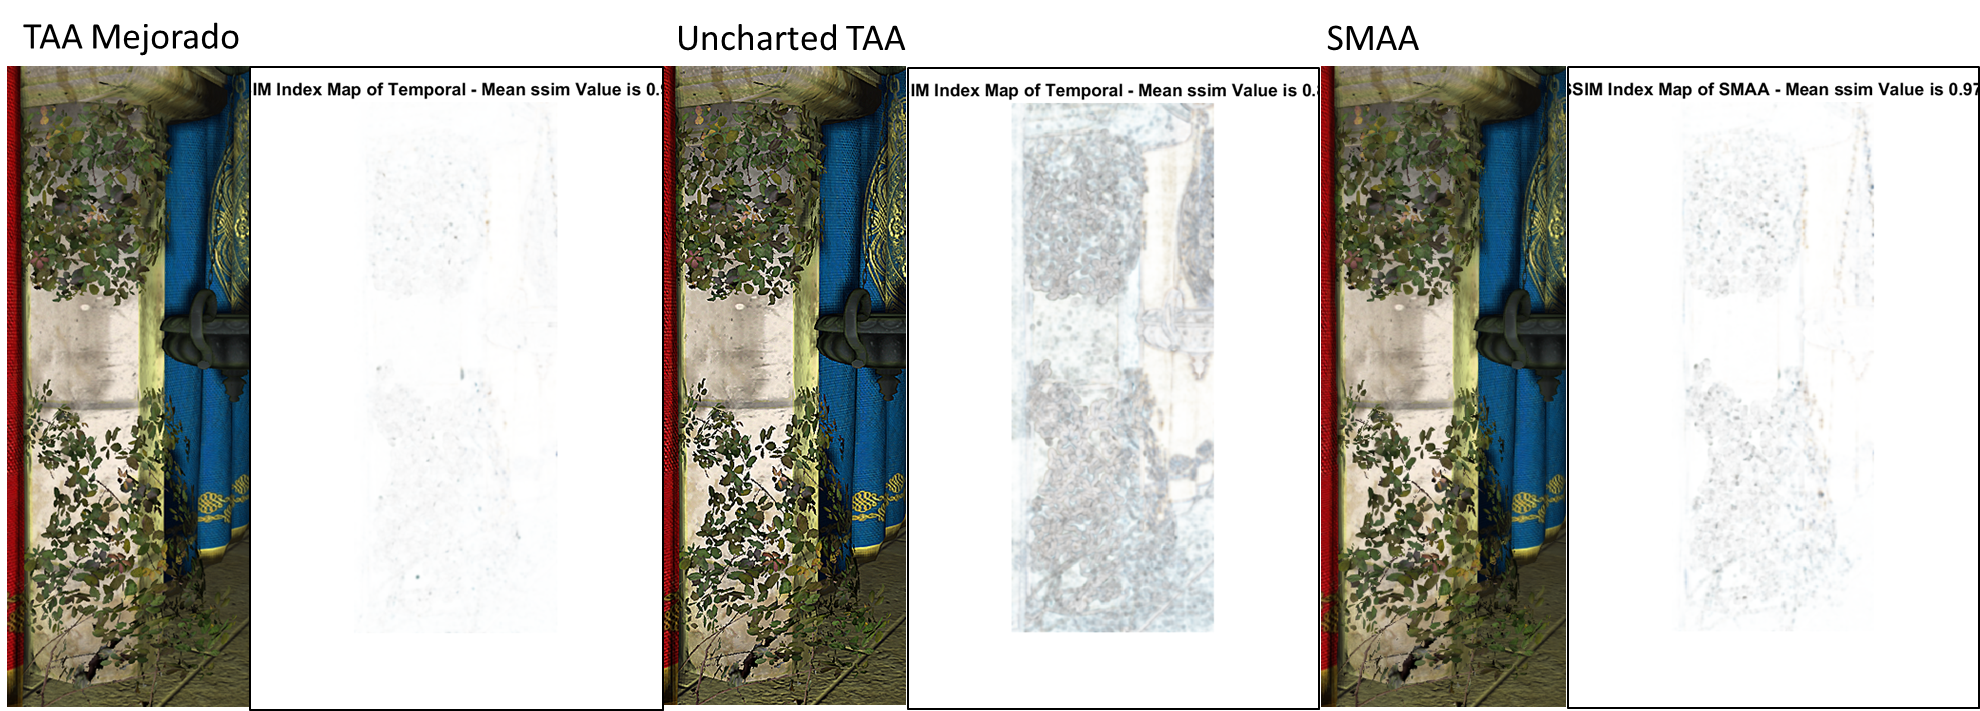
\includegraphics[scale=0.3]{images/results/sponza_flowers.png}
	\caption{Comparación de Prueba de las Flores del Atrium de Sponza entre TAA del Proyecto de Grado, TAA de Uncharted y SMAA.}\label{fig:sponza_flowers_render}
\end{figure}

\FloatBarrier

\subsection{Bordes Duros}
En esta prueba exploramos cómo la implementación del Proyecto de Grado maneja muchos  detalles pequeños a gran distancia y cómo se comporta con bordes duros. Utilizamos los modelos de las Ventanas para los detalles pequeños y los modelos de Tubería y Pared para los bordes duros. 

En las Figuras \ref{fig:hard_test_render} y \ref{fig:hard_test_truth}, observamos que el TAA del Proyecto de Grado es la mejor técnica para manejar los bordes de todos los modelos, su Mapa de SSIM apenas tiene un área oscura y en la Tabla \ref{tab:hard_test} sobrepasa cualquier otra técnica. El TAA de Uncharted crea artefactos de desenfoque alrededor de todos los bordes, esto aparece en su Mapa de SSIM ya que todos los bordes son visibles. Finalmente, SMAA no puede corregir algunos artefactos de \textit{aliasing} que podemos observar en su Mapa de SSIM.

% Table generated by Excel2LaTeX from sheet 'Hard Test'
\begin{table}[!htb]
	\small
	\centering
	\caption{Resultados numéricos de la Prueba de Bordes Duros.}
	\begin{tabular}{l c c c c c c c}
		\hline
		\multicolumn{8}{c}{\textbf{Prueba de Bordes Duros}} \\
		\hline
		\textbf{\diagbox[innerwidth=5em]{Pruebas}{AA}} & \textbf{No AA} & \textbf{FXAA}  & \textbf{SMAA}  & \textbf{\makecell{Uncharted \\ TAA}} & \textbf{\makecell{TAA \\ Mejorado}} & \textbf{Mejor} & \textbf{\makecell{TAA \\ Mejorado \\ Contra \\ El Mejor}} \\
		\hline
		MSE   & 12.463 & 9.342 & 8.019 & 31.385 & 5.012 & \makecell{TAA \\ Mejorado} & 0.000 \\
		
		RMSD  & 3.530 & 3.057 & 2.832 & 5.602 & 2.239 & \makecell{TAA \\ Mejorado} & 0.000 \\
		
		Peak-SNR  & 37.174 & 38.426 & 39.090 & 33.164 & 41.131 & \makecell{TAA \\ Mejorado} & 0.000 \\
		
		SNR   & 30.327 & 31.579 & 32.242 & 26.316 & 34.283 & \makecell{TAA \\ Mejorado} & 0.000 \\
		
		SSIM  & 0.997 & 0.997 & 0.998 & 0.989 & 0.998 & \makecell{TAA \\ Mejorado} & 0.000 \\
		\hline
	\end{tabular}%
	\label{tab:hard_test}%
\end{table}%


\begin{figure}[!htb]
	\centering
	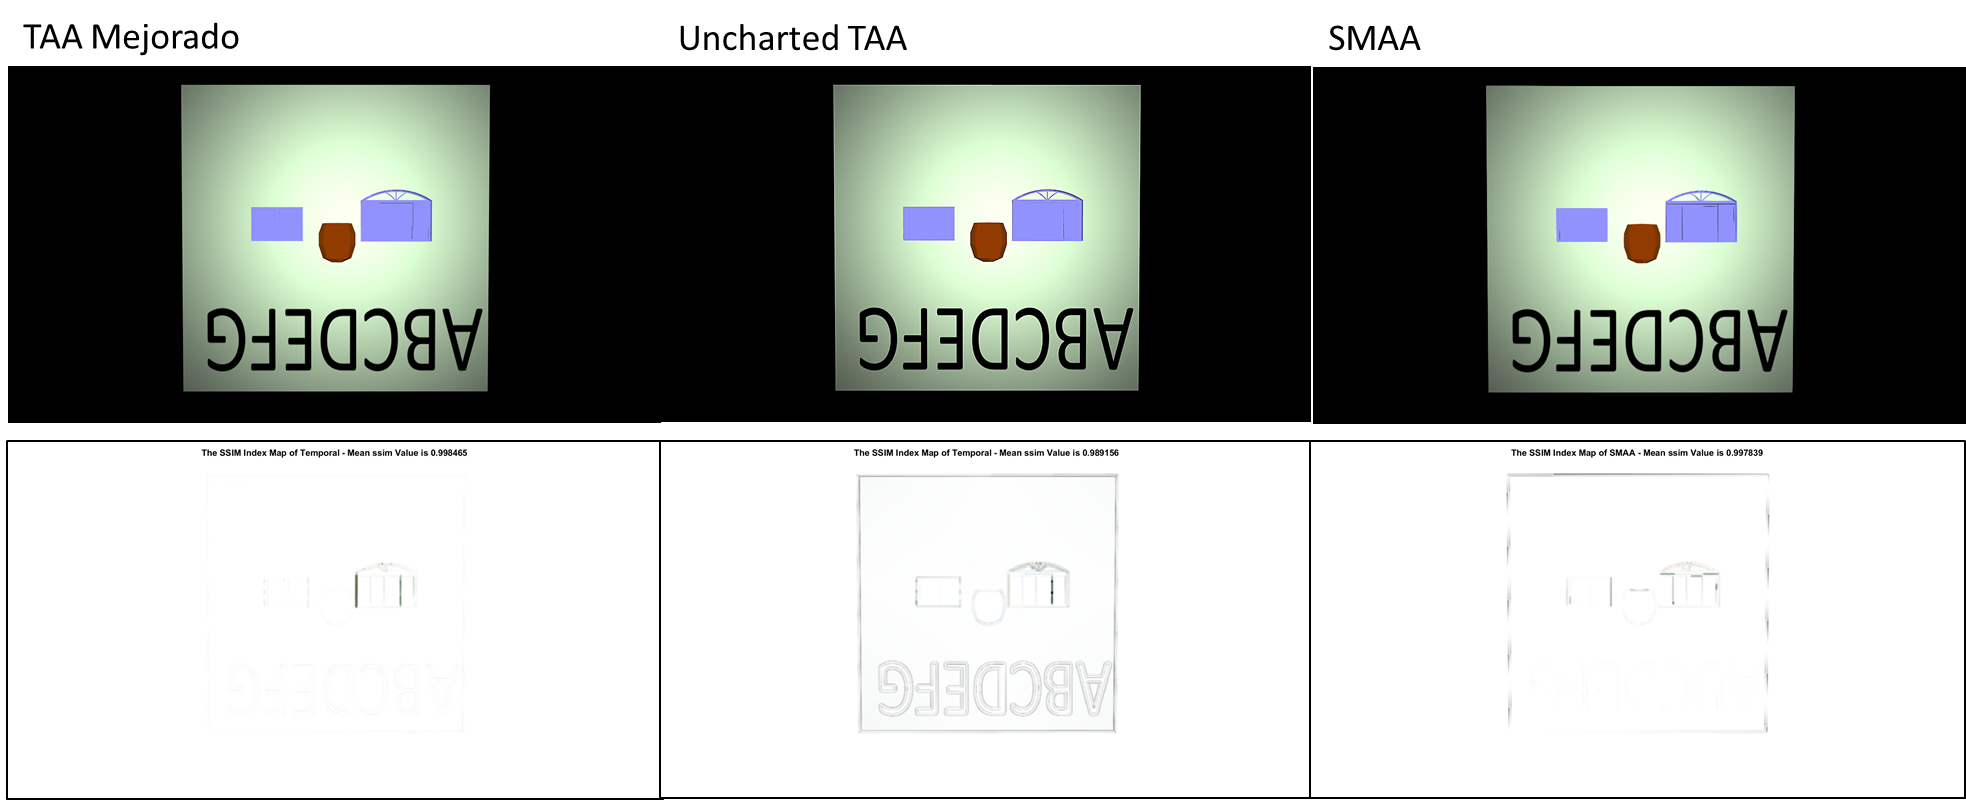
\includegraphics[scale=0.4]{images/results/hard_test.png}
	\caption{Comparación de la Prueba de Bordes Duros entre TAA del Proyecto de Grado, TAA de Uncharted y SMAA.}\label{fig:hard_test_render}
\end{figure}

\begin{figure}[!htb]
	\centering
	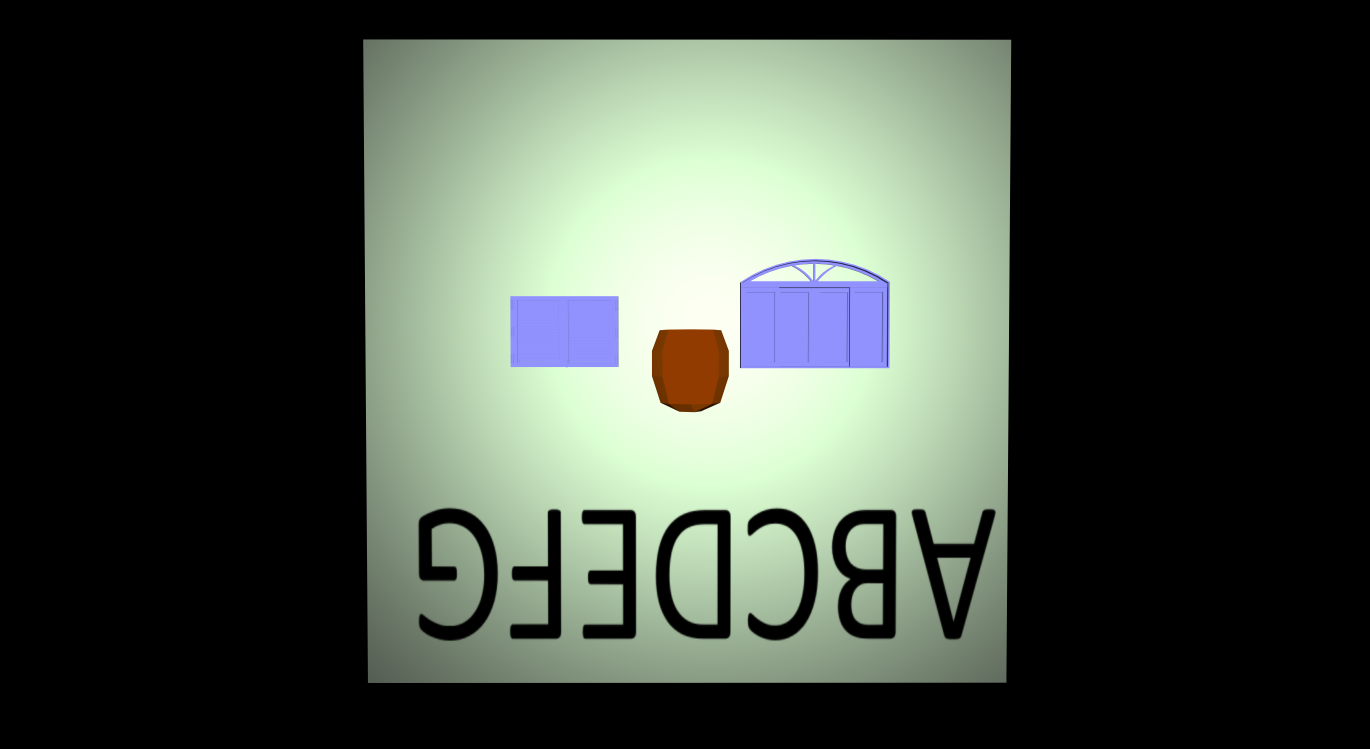
\includegraphics[scale=0.09]{images/results/hard_test_sobel_ground_truth.png}
	\caption{Imagen Base de los Bordes Duros.}\label{fig:hard_test_truth}
\end{figure}

\FloatBarrier

\subsection{Prueba de Ghosting de Esfera}
Con esta prueba queremos medir cómo las mejoras que realizamos disminuyen los efectos de \textit{Ghosting} en las imágenes renderizadas por la implementación de Uncharted. Por esta razón, seleccionamos el Modelo Esfera para que se moviera en la sala del Atrium de Sponza y lo renderizamos bajo un ángulo de cámara que nos mostraba efectos de \textit{Ghosting}.

Como observamos en los resultados visuales de la Figura \ref{fig:sphere_ghosting}, los efectos de  Ghosting disminuyeron en nuestra implementación ya que las franjas visibles en el TAA de Uncharted son casi invisibles en el TAA del Proyecto de Grado. Además, en la Tabla \ref{tab:sphere_ghosting} los resultados promedio en las métricas de imágenes del TAA del Proyecto de Grado son mejores que el promedio del TAA de Uncharted.

Es importante notar que algunas métricas obtuvieron un resultado infinito, ya que eran exactamente iguales a la imagen base; esto sucede en algunas imágenes en las que la esfera cubre todo el cuadro con un color azul oscuro. Es importante señalar que el Índice de Prueba marca a que prueba está asociado el resultado. En los promedios utilizamos No Aplicable (N \\ A) en los resultados para indicar promedio proviene de todas las pruebas, ya que no tiene sentido que se asocie el índice de una prueba específica a ellos. 
% Table generated by Excel2LaTeX from sheet 'Sphere Ghosting'
\begin{table}[!htb]
	\small
	\centering
	\caption{Resumen de resultados numéricos de las 100 pruebas realizadas para la Prueba de \textit{Ghosting} de Esfera.}
	\begin{tabular}{l c c c c}
		\hline
		\multicolumn{5}{c}{\textbf{Resumen de la Prueba de Ghosting de Esfera}} \\
		\hline
		\multicolumn{1}{c}{\textbf{\diagbox{Pruebas}{AA}}} & \textbf{\makecell{Uncharted \\ TAA}} & \textbf{\makecell{Índice \\ de Prueba}} & \textbf{\makecell{TAA \\ Mejorado}} & \textbf{\makecell{Índice \\ de Prueba}} \\
		\hline
		Mejor MSE & 0.000 & 63 & 0.000 & 63 \\
		
		Peor MSE & 100.871 & 19 & 91.766 & 29 \\
		
		Promedio de MSE & 28.634 & N/A   & 19.501 & N/A \\
		
		Mejor Peak-SNR & Inf   & 63 & Inf   & 63 \\
		
		Peor Peak-SNR & 28.093 & 19 & 28.504 & 29 \\
		
		Promedio de Peak-SNR  & Inf   & N/A   & Inf   & N/A \\
		
		Mejor SNR & Inf   & 63 & Inf   & 63 \\
		
		Peor SNR & 16.818 & 11 & 18.524 & 29 \\
		
		Promedio de SNR  & Inf   & N/A   & Inf   & N/A \\
		
		Mejor SSIM & 1.000 & 63 & 1.000 & 63 \\
		
		Peor SSIM & 0.964 & 99 & 0.972 & 29 \\
		
		Promedio de SSIM & 0.965 & N/A   & 0.990 & N/A \\
		\hline
	\end{tabular}%
	\label{tab:sphere_ghosting}%
\end{table}%

\begin{figure}[!htb]
	\centering
	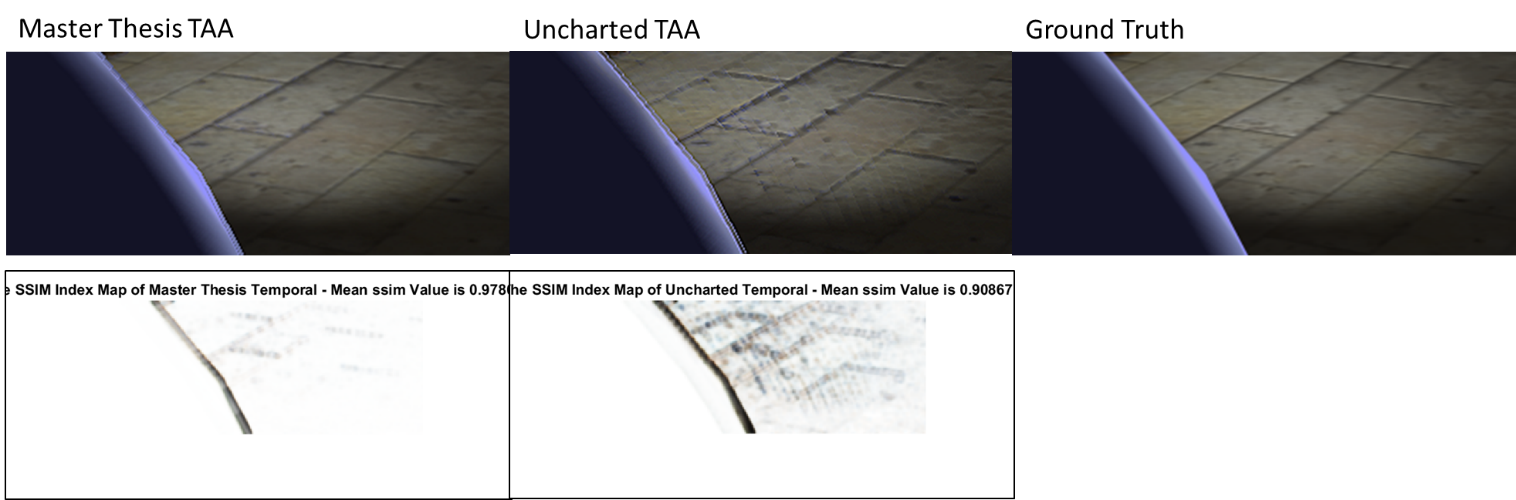
\includegraphics[scale=0.5]{images/results/sphere_ghosting.png}
	\caption{Ejemplo de \textit{Ghosting}. Comparación  entre TAA del Proyecto de Grado y TAA de Uncharted en la Prueba Número 19.}\label{fig:sphere_ghosting}
\end{figure}

\FloatBarrier

\subsection{Hairball}
Estas pruebas fueron las más complicadas para todas las técnicas que probamos. El modelo \textit{Hairball} contiene muchas fibras con muchos detalles, que proporcionan una prueba compleja para cualquier solución de \textit{Anti-Aliasing}. Realizamos pruebas sin luz para ver la silueta y con la luz para ver cómo su reacción a las fibras afectaba a todas las soluciones Anti-Aliasing. Hicimos dos series de pruebas, en la primera, \textit{Hairball} está estático, para mostrarnos el comportamiento de la corrección del desenfoque y \textit{aliasing}. En la segunda serie, \textit{Hairball} gira sobre su propio eje, para mostrarnos cómo se comporta el efecto de \textit{Ghosting} en las fibras. Los resultados de las pruebas estáticas fueron sorprendentes, ya que no esperábamos que la implementación de TAA del Proyecto de Grado fuera el mejor manejo de las fibras debido a los resultados previos en ambas pruebas con las Ventanas, donde los detalles pequeños de las ventanas no se manejan bien.
\subsubsection{Prueba Estática Sin Luz}
En las Figuras \ref{fig:hairball_static_shadow_render} y \ref{fig:hairball_static_shadow_truth}, podemos observar que el TAA de Uncharted tiene problemas en la mayoría de las fibras, en su Mapa de SSIM esto es visible como el gran borde oscuro alrededor de Hairball. SMAA no puede corregir el \textit{aliasing} en las fibras más pequeñas, observamos esto como las áreas grises alrededor del modelo Hairball en su Mapa de SSIM. Finalmente, notamos que el TAA del Proyecto de Grado es la mejor técnica manejando las fibras, las cuales se ven lisas como en el modelo original y en su Mapa de SSIM tiene la menor cantidad de áreas oscuras. Además, en la Tabla \ref{tab:hairball_static_shadow} podemos confirmar que el TAA del Proyecto de Grado es el mejor para renderizar Hairball estático sin luz por un margen relativamente grande, en comparación con las otras técnicas.

% Table generated by Excel2LaTeX from sheet 'Hairball Static Shadow'
\begin{table}[!htb]
	\small
	\centering
	\caption{Resultados numéricos de la Prueba Estática de Hairball Sin Luz.}
	\begin{tabular}{l c c c c c c c}
		\hline
		\multicolumn{8}{c}{\textbf{Prueba Estática de Hairball Sin Luz}} \\
		\hline
		\textbf{\diagbox[innerwidth=5em]{Pruebas}{AA}} & \textbf{No AA} & \textbf{FXAA}  & \textbf{SMAA}  & \textbf{\makecell{Uncharted \\ TAA}} & \textbf{\makecell{TAA \\ Mejorado}} & \textbf{Mejor} & \textbf{\makecell{TAA \\ Mejorado \\ Contra \\ El Mejor}} \\
		\hline
		MSE   & 44.367 & 21.101 & 25.379 & 88.976 & 10.293 & \makecell{TAA \\ Mejorado} & 0.000 \\
		
		RMSD  & 6.661 & 4.594 & 5.038 & 9.433 & 3.208 & \makecell{TAA \\ Mejorado} & 0.000 \\
		
		Peak-SNR  & 31.660 & 34.888 & 34.086 & 28.638 & 38.005 & \makecell{TAA \\ Mejorado} & 0.000 \\
		
		SNR   & 18.808 & 22.036 & 21.234 & 15.786 & 25.154 & \makecell{TAA \\ Mejorado} & 0.000 \\
		
		SSIM  & 0.962 & 0.978 & 0.974 & 0.934 & 0.985 & \makecell{TAA \\ Mejorado} & 0.000 \\
		\hline
	\end{tabular}%
	\label{tab:hairball_static_shadow}%
\end{table}%

\begin{figure}[!htb]
	\centering
	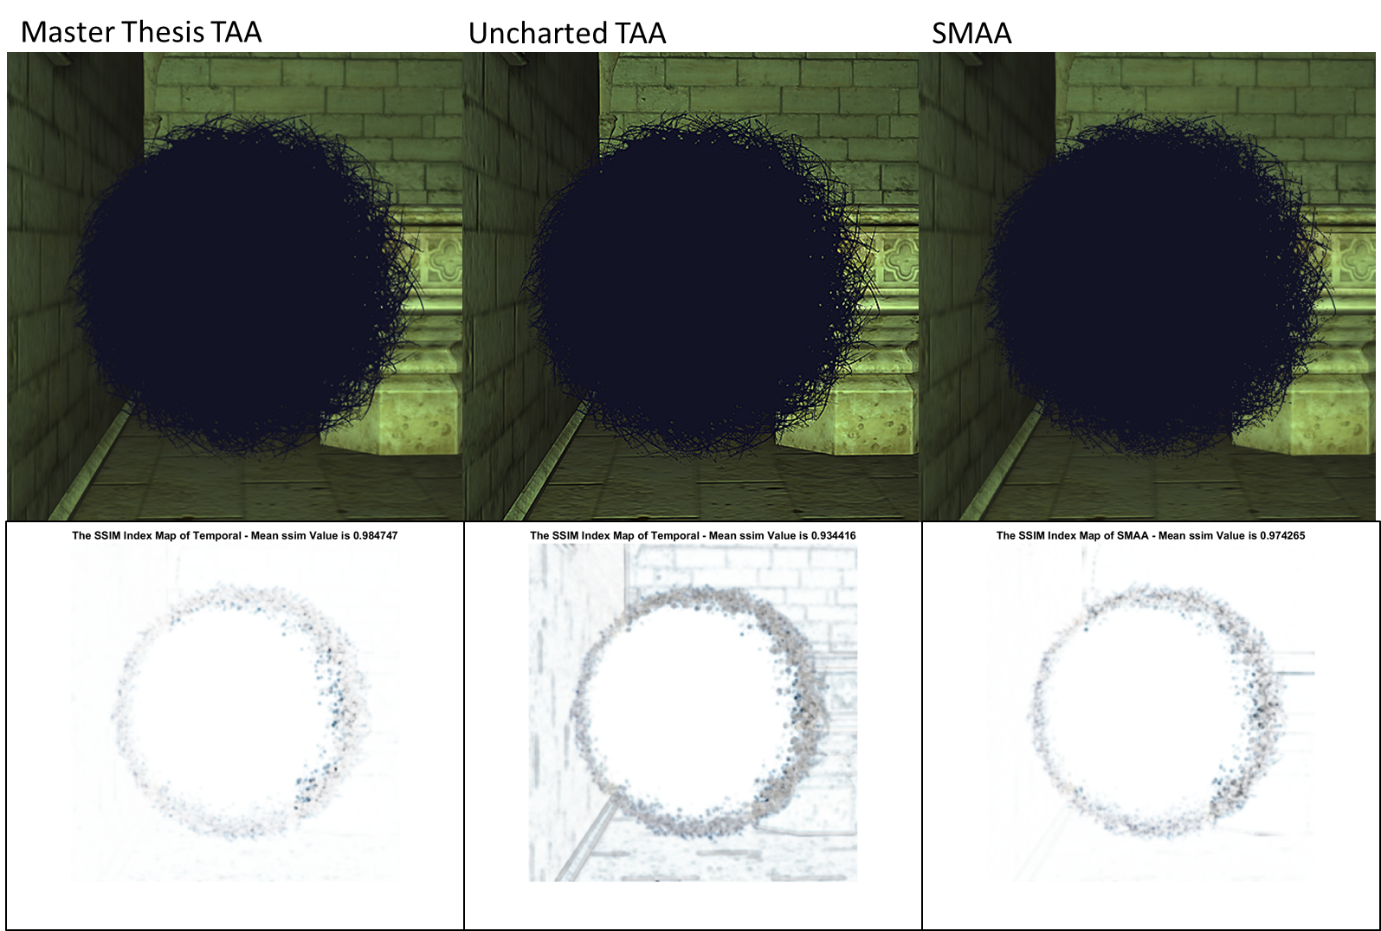
\includegraphics[scale=0.3]{images/results/hairball_static_shadow.png}
	\caption{Comparación de la Prueba Estática de Hairball Sin Luz entre TAA del Proyecto de Grado, TAA de Uncharted y SMAA.}\label{fig:hairball_static_shadow_render}
\end{figure}

\begin{figure}[!htb]
	\centering
	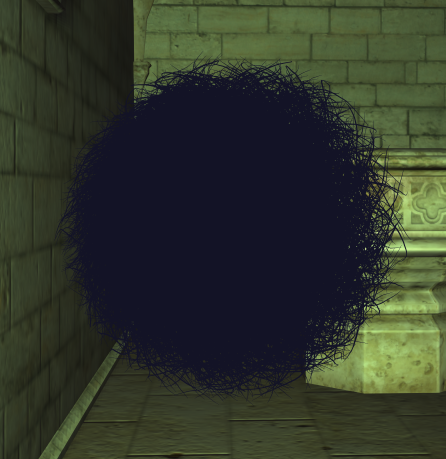
\includegraphics[scale=0.2]{images/results/hairball_sobel_ground_truth.png}
	\caption{Imagen Base de Hairball Estático Sin Luz.}\label{fig:hairball_static_shadow_truth}
\end{figure}

\FloatBarrier

\subsubsection{Prueba Estática Con Luz}
En las Figuras \ref{tab:hairball_static_lighted} y \ref{fig:hairball_static_lighted_truth}, observamos que el TAA de Uncharted generó colores brillantes incorrectos alrededor de todas las fibras, en su Mapa de SSIM esto aparece como el modelo completo oscuro. SMAA no puede corregir una gran cantidad de fibras, aparecen con \textit{aliasing} en la imagen renderizada y su Mapa de SSIM contiene muchas zonas oscuras. Finalmente, podemos observar que el TAA del Proyecto de Grado tiene los bordes más suaves de todas las imágenes renderizadas, en su Mapa SSIM y en la Tabla \ref{tab:hairball_static_lighted} notamos que todavía hay errores pero son más pequeños, por un gran margen, comparado a cualquier otra técnica.

% Table generated by Excel2LaTeX from sheet 'Hairball Static Lighted'
\begin{table}[!htb]
	\small
	\centering
	\caption{Resultados numéricos de la Prueba Estática de Hairball Con Luz.}
	\begin{tabular}{l c c c c c c c}
		\hline
		\multicolumn{8}{c}{\textbf{Prueba Estática de Hairball Con Luz}} \\
		\hline
		\textbf{\diagbox[innerwidth=5em]{Pruebas}{AA}} & \textbf{No AA} & \textbf{FXAA}  & \textbf{SMAA}  & \textbf{\makecell{Uncharted \\ TAA}} & \textbf{\makecell{TAA \\ Mejorado}} & \textbf{Mejor} & \textbf{\makecell{TAA \\ Mejorado \\ Contra \\ El Mejor}} \\
		\hline
		MSE   & 1294.649 & 649.940 & 847.702 & 1444.095 & 226.567 & \makecell{TAA \\ Mejorado} & 0.000 \\
		
		RMSD  & 35.981 & 25.494 & 29.115 & 38.001 & 15.052 & \makecell{TAA \\ Mejorado} & 0.000 \\
		
		Peak-SNR  & 17.009 & 20.002 & 18.848 & 16.535 & 24.579 & \makecell{TAA \\ Mejorado} & 0.000 \\
		
		SNR   & 8.446 & 11.439 & 10.285 & 7.971 & 16.015 & \makecell{TAA \\ Mejorado} & 0.000 \\
		
		SSIM  & 0.801 & 0.865 & 0.841 & 0.785 & 0.937 & \makecell{TAA \\ Mejorado} & 0.000 \\
		\hline
	\end{tabular}%
	\label{tab:hairball_static_lighted}%
\end{table}%

\begin{figure}[!htb]
	\centering
	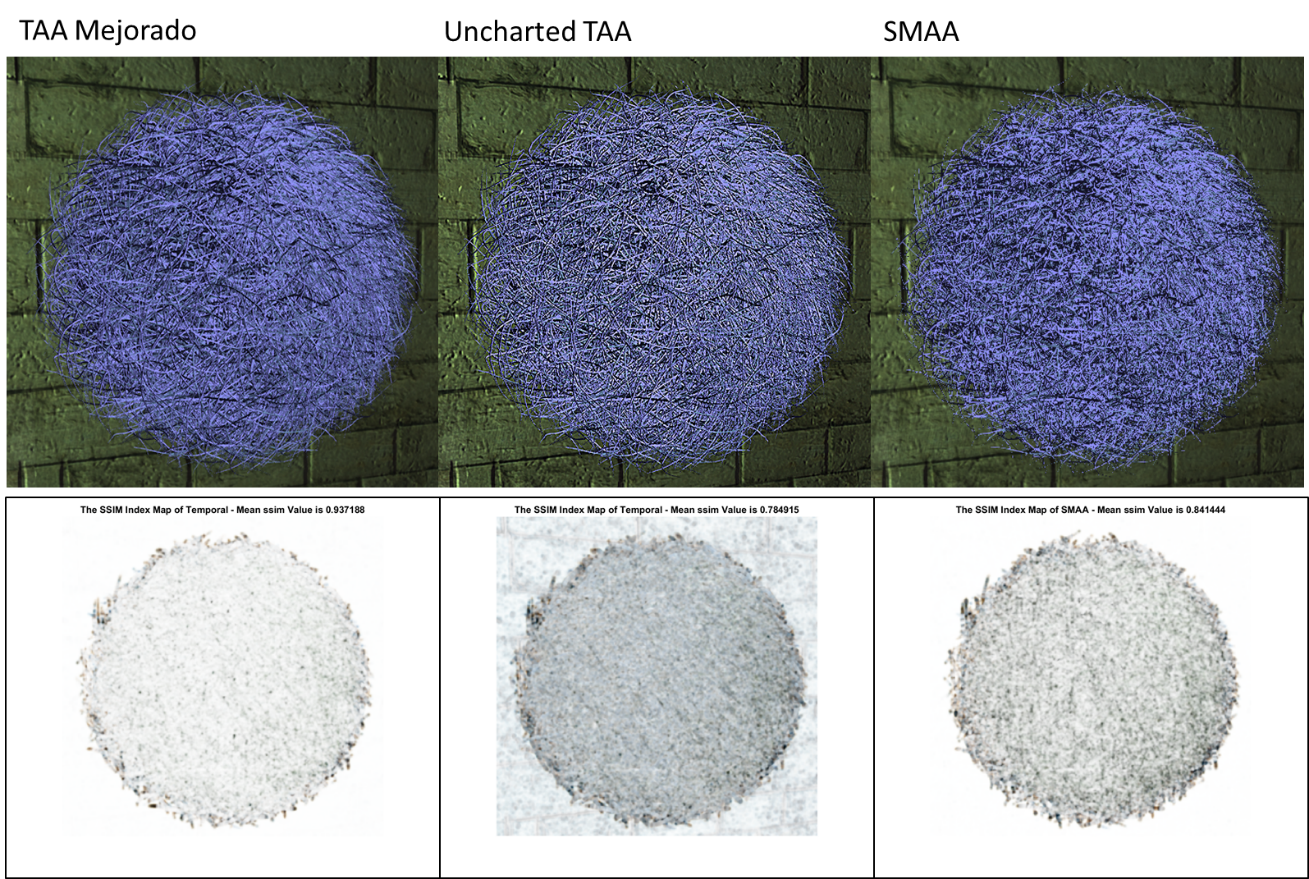
\includegraphics[scale=0.8]{images/results/hairball_static_lighted.png}
	\caption{Comparación de la Prueba Estática de Hairball Con Luz entre TAA del Proyecto de Grado, TAA de Uncharted y SMAA.}\label{fig:hairball_static_lighted_render}
\end{figure}

\begin{figure}[!htb]
	\centering
	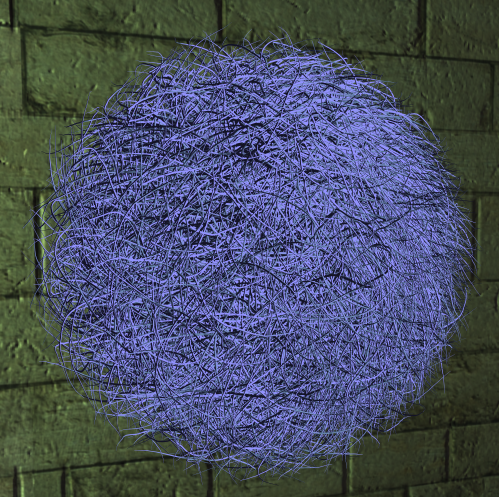
\includegraphics[scale=0.2]{images/results/hairball_light_sobel_ground_truth.png}
	\caption{Imagen Base de Hairball Estático Con Luz.}\label{fig:hairball_static_lighted_truth}
\end{figure}

\FloatBarrier

\subsubsection{Prueba de Ghosting Sin Luz}
En la Figura \ref{fig:hairball_ghosting_shadow}, podemos observar que ambas implementaciones de TAA generan desenfoque alrededor de los bordes de las fibras, esto es visible en ambos Mapas de SSIM como el anillo oscuro alrededor del modelo. En la Tabla \ref{tab:hairball_ghosting_shadow} observamos que el TAA del Proyecto de Grado es numéricamente mejor que el TAA de Uncharted. Además, es importante acotar que el Índice de Prueba en la Tabla \ref{tab:hairball_ghosting_shadow} marca a qué prueba pertenece el resultado asociado; en los promedios que utilizamos No Aplicable (N / A) porque esos resultados provienen del promedio de todas las pruebas y no hace sentido que sea asociado al índice de una prueba específica. 

% Table generated by Excel2LaTeX from sheet 'Hairball Ghosting Shadow'
\begin{table}[!htb]
	\small
	\centering
	\caption{Resumen de resultados numéricos de las 100 pruebas realizadas para la Prueba de \textit{Ghosting} de Hairball Sin Luz.}
	\begin{tabular}{l c c c c}
		\hline
		\multicolumn{5}{c}{\textbf{Resumen de Prueba de Ghosting de Hairball Sin Luz}} \\
		\hline
		\multicolumn{1}{c}{\textbf{\diagbox{Pruebas}{AA}}} & \textbf{\makecell{Uncharted \\ TAA}} & \textbf{\makecell{Índice \\ de Prueba}} & \textbf{\makecell{TAA \\ Mejorado}} & \textbf{\makecell{Índice \\ de Prueba}} \\
		\hline
	    Mejor MSE & 70.261 & 17    & 32.692 & 0 \\
		
		Peor MSE & 93.024 & 90    & 42.962 & 90 \\
		
		Promedio de MSE & 81.887 & N/A   & 38.534 & N/A \\
		
		Mejor Peak-SNR & 29.664 & 17    & 32.986 & 0 \\
		
		Peor Peak-SNR & 28.445 & 90    & 31.800 & 90 \\
		
		Promedio de Peak-SNR  & 29.009 & N/A   & 32.278 & N/A \\
		
		Mejor SNR & 16.940 & 17    & 20.278 & 0 \\
		
		Peor SNR & 15.846 & 90    & 19.201 & 90 \\
		
		Promedio de SNR  & 16.333 & N/A   & 19.602 & N/A \\
		
		Mejor SSIM & 0.925 & 17    & 0.947 & 17 \\
		
		Peor SSIM & 0.911 & 99    & 0.934 & 68 \\
		
		Promedio de SSIM & 0.913 & N/A   & 0.940 & N/A \\
		\hline
	\end{tabular}%
	\label{tab:hairball_ghosting_shadow}%
\end{table}%

\begin{figure}[!htb]
	\centering
	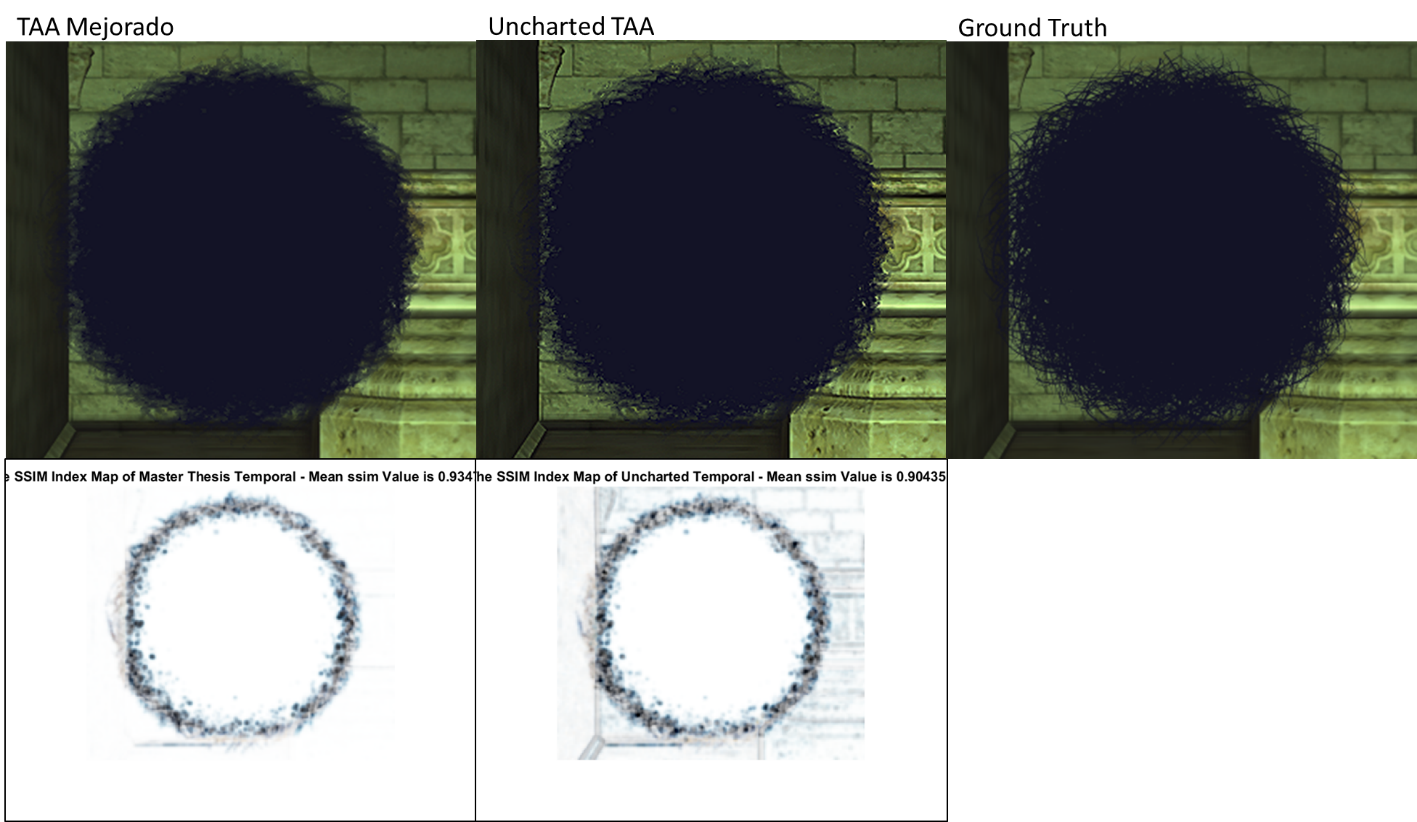
\includegraphics[scale=0.8]{images/results/hairball_ghosting_shadow.png}
	\caption{Comparación de \textit{Ghosting} entre TAA del Proyecto de Grado, TAA de Uncharted y la Imagen Base en la Prueba Número 90.}\label{fig:hairball_ghosting_shadow}
\end{figure}

\FloatBarrier

\subsubsection{Prueba de Ghosting Con Luz}
En la Figura \ref{fig:hairball_ghosting_lighted} y la Tabla \ref{tab:hairball_ghosting_lighted}, observamos que ambas técnicas de TAA generan una gran cantidad de desenfoque alrededor de las fibras. En ambos Mapas de SSIM, el desenfoque es visible ya que Hairball se ve como una gran área oscura. Es importante acotar que el Índice de Prueba en la Tabla \ref{tab:hairball_ghosting_lighted} marca a las que prueba el resultado asociado pertenece; en los promedios que utilizamos No Aplicable (N / A) porque esos resultados provienen del promedio de todas las pruebas.
% Table generated by Excel2LaTeX from sheet 'Hairball Ghosting Lighted'
\begin{table}[!htb]
	\small
	\centering
	\caption{Resumen de resultados numéricos de las 100 pruebas realizadas para la Prueba de \textit{Ghosting} de Hairball Con Luz.}
	\begin{tabular}{l c c c c}
		\hline
		\multicolumn{5}{c}{\textbf{Resumen de Prueba de Ghosting de Hairball Con Luz}} \\
		\hline
		\multicolumn{1}{c}{\textbf{\diagbox{Pruebas}{AA}}} & \textbf{\makecell{Uncharted \\ TAA}} & \textbf{\makecell{Índice \\ de Prueba}} & \textbf{\makecell{TAA \\ Mejorado}} & \textbf{\makecell{Índice \\ de Prueba}} \\
		\hline
		Mejor MSE & 714.811 & 62    & 603.190 & 1 \\
		
		Peor MSE & 980.701 & 83    & 749.516 & 99 \\
		
		Promedio de MSE & 875.687 & N/A   & 671.202 & N/A \\
		
		Mejor Peak-SNR & 19.589 & 62    & 20.326 & 1 \\
		
		Peor Peak-SNR & 18.215 & 83    & 19.383 & 99 \\
		
		Promedio de Peak-SNR  & 18.737 & N/A   & 19.867 & N/A \\
		
		Mejor SNR & 10.037 & 62    & 10.913 & 1 \\
		
		Peor SNR & 8.666 & 83    & 9.902 & 99 \\
		
		Promedio SNR  & 9.261 & N/A   & 10.390 & N/A \\
		
		Mejor SSIM & 0.738 & 62    & 0.766 & 1 \\
		
		Peor SSIM & 0.662 & 99    & 0.694 & 83 \\
		
		Promedio de SSIM & 0.691 & N/A   & 0.722 & N/A \\
		\hline
	\end{tabular}%
	\label{tab:hairball_ghosting_lighted}%
\end{table}%

\begin{figure}[!htb]
	\centering
	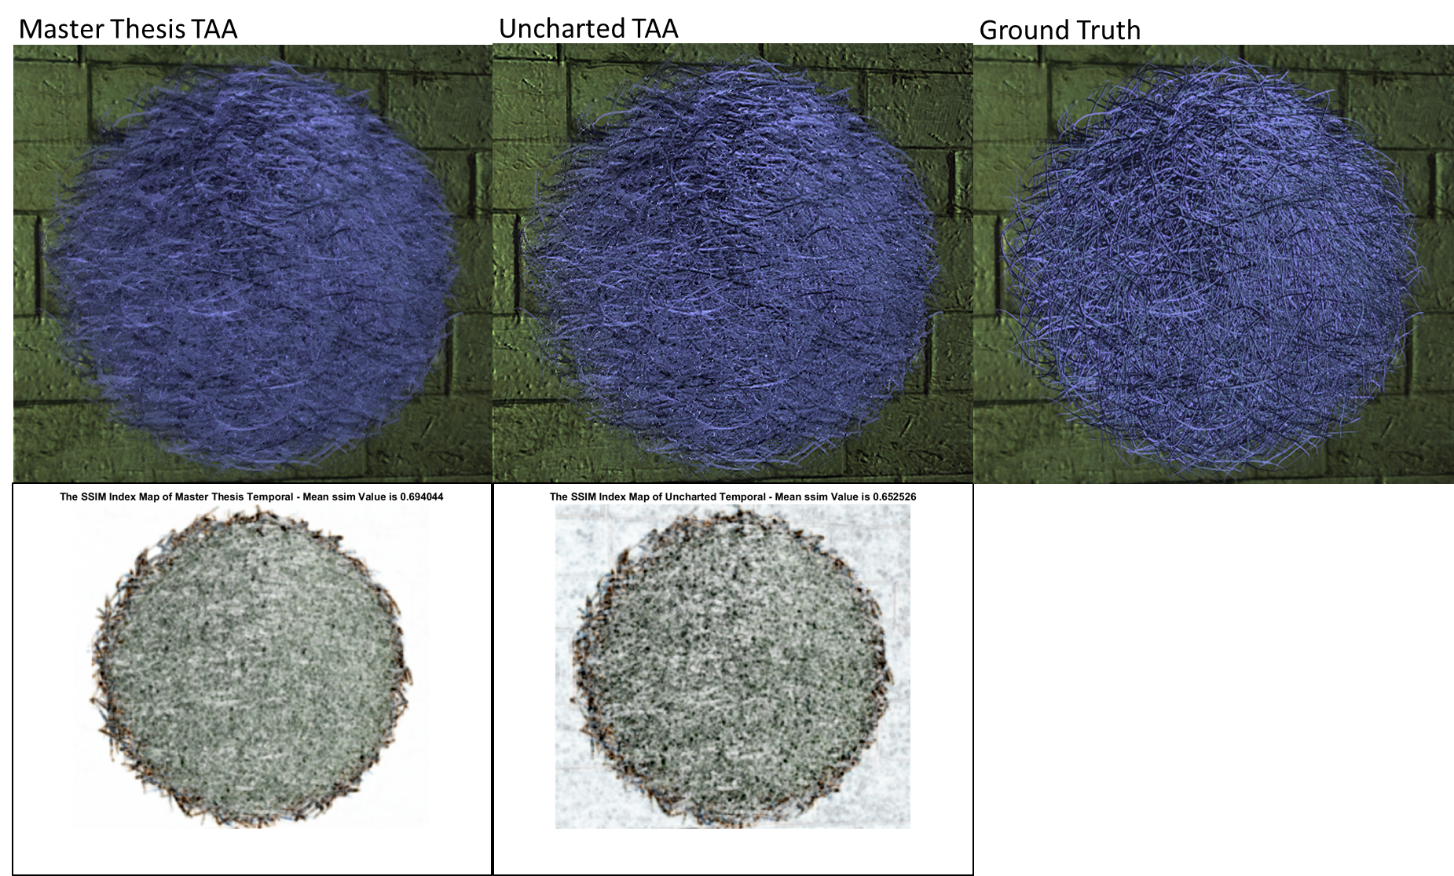
\includegraphics[scale=0.4]{images/results/hairball_ghosting_lighted.png}
	\caption{Comparación de \textit{Ghosting} entre TAA del Proyecto de Grado, TAA de Uncharted y la Imagen Base en la Prueba Número 83.}\label{fig:hairball_ghosting_lighted}
\end{figure}

\FloatBarrier
\subsection{Comparación de Tiempos} \label{result_timing}
Es importante tener en cuenta que todas las técnicas probadas son de naturaleza de Post-Procesamiento, lo que significa que reciben la imagen de salida de la Arquitectura de \textit{Shading} Diferido como entrada y no dependen de la complejidad de la escena.

El tiempo medido que tomó la técnica de TAA del Proyecto de Grado fue entre $0.5$ y $0.6$ $ms$ en promedio. El paso de Sobel tomó entre $0.2$ $ms$ y $0.3$ $ms$, y la reproyección fue de alrededor de $0.3$ $ms$. El tiempo medido que tomó la técnica TAA de Uncharted fue de entre $0.2$ $ms$ y $0.3$ $ms$; FXAA tomó entre $0.1$ $ms$ y $0.2$ $ms$; y SMAA tomó $0.2$ $ms$ y $0.3$ $ms$.


\section{Discusión}
Como apreciamos los resultados de la prueba del Filtro de Nitidez, ver Tabla \ref{tab:sharpen_res}, las mejoras logradas en este proyecto de grado van más allá de modificar el filtro de la implementación de Uncharted, ya que al cambiar este filtro sólo se evita generar esos píxeles brillantes incorrectos alrededor bordes. Creemos que el uso de ese filtro específico es de naturaleza artística, ya que tiende a pronunciar los bordes a costa de crear píxeles brillantes, que parpadean al moverse, alrededor de los bordes. Esto es especialmente notable cuando la cámara se mueve, mientras el primer plano está iluminado pero el fondo está en sombras o viceversa.

De ambas Ppuebas de Tubería, podemos observar que los resultados del TAA del Proyecto de Grado están cerca de los resultados de SMAA al dibujar bordes duros. Podemos cuantificar la reducción del problema del desenfoque al comparar con la implementación de TAA de Uncharted en los resultados de las Tablas \ref{tab:pipe_regular} y \ref{tab:pipe_inclination}. Cuando comparamos los resultados de los Mapas de SSIM (Figuras \ref{fig:pipe_regular_render} y \ref{fig:pipe_inclination_render}), observamos una gruesa línea de error alrededor de los bordes en la implementación de Uncharted, la cual no está presente en nuestra implementación. Pero la reducción del desenfoque no es perfecta, como vemos en los puntajes de las pruebas, aun aparece alrededor de los bordes de nuestra implementación y le permite a SMAA obtener el puntaje más alto en algunas pruebas.

De las pruebas de Ventanas con Persianas y Ventana Arqueada, podemos apreciar cómo reaccionan las técnicas ante características pequeñas, casi de tamaño de píxel, como las persianas y las puertas de las ventanas de las pruebas. Aunque el TAA del Proyecto de Grado y SMAA aparecen numéricamente mejores que el TAA de Uncharted en las Tablas \ref{tab:window_blind} y \ref{tab:window_arch}, no pueden reconstruir todos los pequeños detalles y dejan rayas finas de píxeles que parpadean cuando la cámara se mueve. Creemos que, en este caso, admitir el desenfoque del TAA de Uncharted beneficia su aplicación final porque es mejor perder algunos pequeños detalles que tener muchos píxeles parpadeando cada vez que se mueve la cámara.

La Prueba del Atrium de Sponza nos muestra que el TAA del Proyecto de Grado es más que capaz de manejar una escena general con iluminación y sombras. Como se ve en la Tabla \ref{tab:sponza}, nuestra implementación demostró ser mejor que las otras técnicas \textit{Anti-Aliasing} por un margen justo en casi todas las pruebas.

Consideramos que la prueba de las Flores del Atrium de Sponza un experimento distinto al resto, pues las flores son una superficie plana 2D con muchos agujeros transparentes complejos que giran alrededor de la columna. Como observamos a partir de los resultados numéricos de la Tabla \ref{tab:sponza_flowers} y los Mapas de SSIM en la Figura \ref{fig:sponza_flowers_render}, todas las técnicas tienen problemas con esos agujeros transparentes, pero nuestro implementación de TAA demuestra ser el mejor en el manejo ellos. Vemos en esta prueba que nuestra implementación es buena para manejar este tipo de pequeños detalles que, en comparación con las pruebas de las Ventanas, son más grandes que solo un píxel. 

A partir de la prueba de Bordes Duros, seguimos observando que la técnica del Proyecto de Grado maneja mejor el desenfoque, en comparación al TAA de Uncharted (ver Tabla \ref{tab:hard_test}), esto es especialmente notable en las letras, la tubería y el cuadrado. También notamos que la técnica del Proyecto de Grado todavía tiene dificultades para manejar los detalles súper finos de las ventanas, a esta distancia todavía creemos que el desenfoque del TAA Uncharted ayuda a ocultar las rayas de píxeles no deseados, que parpadean al ocurrir movimiento(Ver Figura \ref{fig:hard_test_render}).

En la prueba de \textit{Ghosting} de Esfera, vemos un claro ejemplo de las mejoras logradas en este proyecto de grado. La Figura \ref{fig:sphere_ghosting} muestra un ejemplo del efecto de \textit{Ghosting} creado por la implementación del TAA de Uncharted, podemos percibir claramente las franjas que deja la esfera mientras se mueve, mientras que en nuestra implementación de TAA son apenas visibles.

Finalmente, tenemos las cuatro pruebas de Hairball, que fueron las más complejas realizadas en este proyecto de grado. El modelo Hairball tiene muchos huecos y pequeños detalles que reaccionan a la iluminación y las sombras. Anticipamos una gran cantidad de errores debido a ellos porque todas las técnicas \textit{Anti-Aliasing} tienen dificultades para reconstruir esta alta densidad de detalles finos.

En la prueba Estática Sin Luz y la prueba Estática Con Luz (Ver Tablas \ref{tab:hairball_static_shadow} y \ref{tab:hairball_static_lighted}) podemos observar que la implementación del Proyecto de Grado es la mejor para renderizar las fibras de cabello. Es capaz de reconstruir bordes más suaves que el TAA de Uncharted y reconstruye más detalles que SMAA. Especialmente, en la versión con luz (Ver Figura \ref{fig:hairball_static_lighted_render}), podemos apreciar qué tan suave es el resultado; se ve casi como la imagen de referencia. Esta prueba superó, con creces, nuestra expectativa de las mejoras. Los resultados visuales y numéricos (Ver tabla \ref{tab:hairball_static_lighted}) muestran un gran aumento en la calidad en comparación con las otras soluciones \textit{Anti-Aliasing}.

En la prueba de \textit{Ghosting} Sin Luz y Con Luz, observamos que los resultados de ambas técnicas presentan desenfoque en exceso (Ver Figuras \ref{fig:hairball_ghosting_shadow} y \ref{fig:hairball_ghosting_lighted}), especialmente la implementación de la TAA del Proyecto de Grado en la versión con luz. Creemos que esto es causado porque el Buffer de Historia y Pase Temporal de Sobel que no pueden estabilizarse tan rápido como la velocidad de cambio de los colores cuando las fibras se mueven; esto es, el rechazo de color es más lento de lo necesario. Los valores numéricos de las Tablas \ref{tab:hairball_ghosting_shadow} y \ref{tab:hairball_ghosting_lighted} confirman los efectos del desenfoque, dado que el MSE es más alto de lo normal.


A partir de nuestros resultados de la comparación de tiempos (Consulte la sección \ref{result_timing}), podemos ver que nuestras mejoras se ajustan a los requisitos de tiempo para ejecutarse en aplicaciones en tiempo real, ya que está por debajo del límite común de $1$ $ms$.


\chapter{Conclusiones y Recomendaciones}
Como hemos demostrado numérica y visualmente con las pruebas realizadas, la implementación Mejorada del Proyecto de Grado logró su objetivo de reducir los efectos de desenfoque y los efectos de \textit{Ghosting} de la técnica \textit{Temporal Anti-Aliasing}, con el uso de detección de bordes de color y profundidad e indexación de triángulos. Nuestros resultados muestran que esta técnica puede proporcionar la misma o mejor calidad que otras soluciones estándar de \textit{Anti-Aliasing}.

Como posibles mejoras, creemos en que nuestra implementación podría optimizarse para ejecutarse más rápido que nuestro tiempo actual. Nuestra implementación se realizó con flexibilidad en mente, para ayudarnos a probar diferentes enfoques. Esto podría simplificarse para reducir el número de etapas requeridas.

En cuanto a las recomendaciones para futuras investigaciones, sugerimos mejorar el comportamiento de la técnica bajo objetos en movimiento con alta densidad de detalles, como en las pruebas de Hairball. Otro tema de mejora es la estabilidad de los detalles del tamaño de un píxel, que causan parpadeos como en las pruebas de Ventanas. Además, todavía se requiere una solución de \textit{Anti-Aliasing} de Iluminación Especular compatible con \textit{Temporal Anti-Aliasing} para proporcionar una solución de rango completo al \textit{Aliasing} en aplicaciones en tiempo real. Asimismo, sugerimos buscar métricas de imagen más específicas para gráficos por computadora, especialmente, encontrar valores de ajuste para SSIM que proporcionen una resolución numérica mayor al comparar diferentes imágenes procesadas


\bibliography{MyMSc}

\appendix
\chapter{Repositorio de GitHub}
El enlace principal al repositorio es https://github.com/maniatic0/Christian-TRAA . Desde allí, se puede acceder a los siguientes enlaces para la versión impresa de este informe.
\begin{itemize}
	\item Repositorio Completo: \url{https://github.com/maniatic0/Christian-TRAA}.
	\item Especificación Completa de la Computadora: \\ \url{https://github.com/maniatic0/Christian-TRAA/tree/master/PC%20Specification}.
	\item Todas las Pruebas: \\ \url{https://github.com/maniatic0/Christian-TRAA/tree/master/Important%20Tests}.
	\item Pruebas del Buffer de Acumulación: \\ \url{https://github.com/maniatic0/Christian-TRAA/tree/master/Important%20Tests/Accumulation%20Buffer%20Tests}.
	\item La Mayoría de las Pruebas del Proyecto de Grado: \\ \url{https://github.com/maniatic0/Christian-TRAA/tree/master/Important%20Tests/Master%20Thesis%20Tests}.
	\item Pruebas del Filtro de Nitidez: \\ \url{https://github.com/maniatic0/Christian-TRAA/tree/master/Important%20Tests/Sharpening%20Tests}.
	\item Pruebas de \textit{Ghosting}: \\ \url{https://github.com/maniatic0/Christian-TRAA/tree/master/Important%20Tests/Ghosting}.
	\item Pruebas de HairBall: \\ \url{https://github.com/maniatic0/Christian-TRAA/tree/master/Important%20Tests/HairBall}.
	\item Código: \\ \url{https://github.com/maniatic0/Christian-TRAA/tree/master/CG_Labs}.
	\item Reporte de \LaTeX: \\ \url{https://github.com/maniatic0/Christian-TRAA/tree/master/LaTeX/Master_Thesis_Spanish}.
\end{itemize}
\chapter{Explicación del Camera Jittering} \label{appendix:jitter}
La Secuencia de $Halton(2, 3)$ genera puntos en el espacio $[0,1] \times [0,1]$. Primero, tenemos que transformarlo en el espacio $[- 1,1] \times [-1,1]$ porque consideramos que el píxel está en el centro, es decir, en OpenGL, el primer píxel está en $(0.5, 0.5)$. Por esto, aplicamos la transformación $T_1 (x, y) = 2 * (x, y) - (1, 1)$.

Ahora, solo queremos causar \textit{jittering} dentro del píxel porque solo deberíamos tomar muestras dentro de él. Queremos controlar este movimiento, pero para fines de explicación, podemos suponer que solo lo estarems dentro del píxel. Entonces, aplicamos la transformación $T_2 (x, y) = \frac{(x, y)}{2}$.

A partir de ahora, debemos cambiar la forma en que interpretamos el proceso que estamos realizando; estamos calculando la distancia a la que moveremos el centro de píxeles, por lo que debemos verlo como un vector en lugar de como un punto. Necesitamos transformar el vector en un vector normalizado por el tamaño de la pantalla. En consecuencia, aplicamos la transformación $T_3 (x, y) = (x, y) / (w, h)$ con $(w, h)$ siendo el ancho y alto de la pantalla y el operador "$/$" como división por componentes.

Ahora necesitamos transformar nuestro vector normalizado por el tamaño de pantalla $ [0, 1] $ a las Coordenadas Normalizadas del Dispositivo (\textit{Normalized Device Coordinates}, NDC) que van en el rango $ [- 1, 1] \times [-1, 1]$. Esto se hace usando la transformación $T_4 (x, y) = 2 * (x, y)$ (para transformar puntos, usaríamos $2 * (x, y) - (1, 1)$). Al final, nuestra transformación se vería así $T (x, y) = T_4 (T_3 (T_2 (T_1 (x, y)))) = (2 * (x, y) - (1, 1)) / (w, h) $ con $ (x, y) $ siendo un punto de la Secuencia de Halton.

Ahora necesitamos modificar nuestra Matriz de Proyección, que toma puntos del espacio de visualización en el Espacio de Clip (\textit{Clip Space}, donde se eliminan fácilmente los vértices trivialmente no visibles). La matriz resultante se toma de la página 14 de presentación de Ke Xu ~\cite{XU2016}. Sea $ (h_x, h_y) $ el \textit{jittering} que hemos calculado previamente.

\begin{equation}
\begin{split}
JitteredProjection = & \begin{bmatrix*} 
a & 0 & h_x & 0 \\ 
0 & b & h_y & 0 \\
0 & 0 & c & d   \\
0 & 0 & -1 & 0   \end{bmatrix*} = JitterMatrix\times Projection \\
= & \begin{bmatrix*} 
1 & 0 & 0 & -h_x \\ 
0 & 1 & 0 & -h_y \\
0 & 0 & 1 & 0   \\
0 & 0 & 0 & 1   \end{bmatrix*} \times \begin{bmatrix*} 
a & 0 & 0 & 0 \\ 
0 & b & 0 & 0 \\
0 & 0 & c & d   \\
0 & 0 & -1 & 0   \end{bmatrix*}
\end{split}
\end{equation}

Veamos su efecto a un punto en el \textit{View Space} (visión desde perspectiva de la cámara), sea $p_{view}=(x,y,z,1)$.

\begin{equation}
	JitteredProjection\times p_{view} = \begin{bmatrix*}
	a*x+h_x*z \\
	b*y+h_y*z \\
	c*z+d \\
	-z
	\end{bmatrix*}
\end{equation}

Procedemos a hacer la \textit{División en Perspectiva} (corrige la perspectiva a la deseada en la cámara) para transformar el punto en Coordenadas NDC, esto se logra dividiendo el vector por el componente w. 

\begin{equation}
\begin{bmatrix*}
-a*\frac{x}{z}-h_x \\
-b*\frac{y}{z}-h_y \\
-c+\frac{d}{z}d \\
1
\end{bmatrix*} = p_{NDC} + \begin{bmatrix*}
-h_x \\
-h_y \\
0 \\
0
\end{bmatrix*}
\end{equation}

En consecuencia, solo necesitamos estar seguros de que podemos aplicar la Matriz de \textit{Jittering}, para usarla dentro de \textit{Pixel Shaders}, con puntos en el espacio NDC.

\begin{equation}
	JitterMatrix\times p_{NDC} = \begin{bmatrix*}
	x_{NDC}-h_x \\
	y_{NDC}-h_y \\
	z_{NDC} \\
	1
	\end{bmatrix*} = p_{NDC} + \begin{bmatrix*}
	-h_x \\
	-h_y \\
	0 \\
	0
	\end{bmatrix*}
\end{equation}

\end{document}